\RequirePackage{fix-cm}
\documentclass[12pt, table, letterpaper]{report}

%%%%%%%%%%%%%%%%%%%%%%%%%%%%%%%%%%%%%
% Document configuration
\usepackage[english,spanish,es-tabla]{babel}
\usepackage[
	letterpaper,
	top = 18mm,
	left = 20mm,
	right= 20mm,
	bottom = 18mm
]{geometry}

\usepackage{ragged2e}
\usepackage{fancyhdr}
\usepackage{lastpage}	
\usepackage{multicol}
%%%%%%%%%%%%%%%%%%%%%%%%%%%%%%%%%%%%%

%%%%%%%%%%%%%%%%%%%%%%%%%%%%%%%%%%%%%
% Fonts, encoding & Color
\usepackage{fontspec}
\usepackage{titlesec}
%\usepackage{xunicode}

\usepackage[table]{xcolor}
\usepackage[shortlabels]{enumitem}
\usepackage{epigraph}
%%%%%%%%%%%%%%%%%%%%%%%%%%%%%%%%%%%%%

%%%%%%%%%%%%%%%%%%%%%%%%%%%%%%%%%%%%%
% Math & chem

\usepackage{amsmath}
\usepackage{amsfonts}
\usepackage{siunitx}
\usepackage{xfrac}
\usepackage[
	modules={reactions,formula,redox,charges}
]{chemmacros}[2022/03/11]
%\usepackage{chemformula}
%%%%%%%%%%%%%%%%%%%%%%%%%%%%%%%%%%%%%

%%%%%%%%%%%%%%%%%%%%%%%%%%%%%%%%%%%%%
% Figures & tables

\usepackage{graphicx}
\usepackage[justification=centering]{caption}
\usepackage{subcaption}
\usepackage{floatrow}
\usepackage{wrapfig}

\usepackage{tabularray}
\UseTblrLibrary{varwidth}
\UseTblrLibrary{siunitx}
%%%%%%%%%%%%%%%%%%%%%%%%%%%%%%%%%%%%%

%%%%%%%%%%%%%%%%%%%%%%%%%%%%%%%%%%%%%
% Drawings & shapes

\usepackage{tikz}
\usetikzlibrary{
	shapes.geometric,
	positioning,
	arrows.meta,
	calc,
	patterns,
	patterns.meta,
	shadows,
	matrix
}

\usepackage[most]{tcolorbox}
\tcbuselibrary{raster}
\tcbuselibrary{external}
\tcbset{external/prefix=Boxes/}
\tcbEXTERNALIZE

\usepackage[edges,external]{forest}
\usepackage{chemplants}

\usetikzlibrary{external}
\tikzexternalize[prefix=Pictures/]
%%%%%%%%%%%%%%%%%%%%%%%%%%%%%%%%%%%%%

%%%%%%%%%%%%%%%%%%%%%%%%%%%%%%%%%%%%%
% Bibliography, glossary & refs

\usepackage[
	hidelinks
]{hyperref}
\usepackage[spanish]{cleveref}
\usepackage[
	toc,
	acronym,
	symbols,
	translate = true,
]{glossaries}
\usepackage{glossary-mcols}

\usepackage[
	thresholdtype=words
]{csquotes}

\usepackage[
	backend=biber,
	style=ieee,
	url=false,
	hyperref=true,
]{biblatex}

\usepackage{xurl}
%%%%%%%%%%%%%%%%%%%%%%%%%%%%%%%%%%%%%

%%%%%%%%%%%%%%%%%%%%%%%%%%%%%%%%%%%%%
% utils

\usepackage{adjustbox}
\usepackage{pdfpages}
%\usepackage[some]{background}
%%%%%%%%%%%%%%%%%%%%%%%%%%%%%%%%%%%%%
%%%%%%%%%%%%%%%%%%%%%%%%%%%%%%%%%%%%%
% Language & localization

\selectlanguage{spanish}
\crefname{table}{\spanishtablename}{\spanishtablename}
\crefname{reaction}{reacción}{reacciones}
\Crefname{Reaction}{Reacción}{Reacciones}
\crefname{section}{sección}{secciones}
\crefname{Section}{Sección}{Secciones}
\crefname{figure}{fig.}{figs.}
\Crefname{figure}{Fig.}{Figs.}
\decimalpoint
%%%%%%%%%%%%%%%%%%%%%%%%%%%%%%%%%%%%%

%%%%%%%%%%%%%%%%%%%%%%%%%%%%%%%%%%%%%
% Math & chem

%\newcommand*\fancyrefrctlabelprefix{rct}
\chemsetup{
	reactions/own-counter = true
}

\sisetup{
	per-mode = symbol,
	sticky-per
}

\DeclareSIUnit\day{day}
%%%%%%%%%%%%%%%%%%%%%%%%%%%%%%%%%%%%%

%%%%%%%%%%%%%%%%%%%%%%%%%%%%%%%%%%%%%
% Table

%\UseTblrLibrary{booktabs, siunitx}

\DefTblrTemplate{contfoot-text}{normal}{Continúa en la siguiente página}
\DefTblrTemplate{conthead-text}{normal}{(Continuación)}
\SetTblrTemplate{conthead-text}{normal}
\SetTblrTemplate{contfoot-text}{normal}

%\newcommand{\xltmulticolumn}[3]{
%	\multicolumn{#1}
%	{|>{\hsize=\dimexpr#1\hsize+\tabcolsep * (2 * (#1 - 1) )+\arrayrulewidth* (#1 - 2)\relax}#2|}
%	{#3}
%}
%%%%%%%%%%%%%%%%%%%%%%%%%%%%%%%%%%%%%

%%%%%%%%%%%%%%%%%%%%%%%%%%%%%%%%%%%%%
% Fonts, list & titles

\setlength{\parindent}{0pt}
\setlength{\parskip}{1em}

\defaultfontfeatures{Ligatures=TeX}
\setmainfont{Times New Roman}

\titleformat{\chapter}[display]
    {\normalfont\huge\bfseries}{\chaptertitlename\ \thechapter}{20pt}{\Huge}
\titlespacing*{\chapter}{0pt}{0pt}{0pt}

% Define a new Font family, use only if it doesn't recognize your fonts

\newfontfamily{\BellMT}{Bell MT}[
	Extension = .ttf,
	Path = /usr/share/fonts/bell-mt/,
	BoldFont = BELLB,
	ItalicFont = BELLI
]

\newfontfamily{\Footlight}{FTLTLT}[
	Extension = .ttf,
	Path = /usr/share/fonts/Footlight-MT/,
	BoldFont = footlight-mt-bold
]

%% Custom section

%\setcounter{tocdepth}{3}
%\titleclass{\subsubsection}{straight}[\subsection]
%\newcounter{subsubsection}[subsection]
%\renewcommand\thesubsubsection{\thesubsection.\arabic{subsubsection}}

%\titleclass{\subsubsubsection}{straight}[\subsection]
%\newcounter{subsubsubsection}[subsubsection]
%\renewcommand\thesubsubsubsection{\thesubsubsection.\arabic{subsubsubsection}}
%
%\titleformat{\section}{\normalfont\fontsize{16}{15}\bfseries}{\thesection}{1em}{}
%\titleformat{\subsection}{\normalfont\fontsize{14}{15}\bfseries}{\thesubsection}{1em}{}
%\titleformat{\subsubsection}{\normalfont\fontsize{14}{15}\bfseries}{\thesubsubsection}{1em}{}
%\titleformat{\subsubsubsection}{\normalfont\fontsize{14}{15}\bfseries}{\thesubsubsubsection}{1em}{}
%
%\titlespacing\section{0pt}{12pt plus 4pt minus 2pt}{0pt plus 2pt minus 2pt}
%\titlespacing\subsection{0pt}{10pt plus 4pt minus 2pt}{0pt plus 2pt minus 2pt}
%\titlespacing\subsubsection{0pt}{10pt plus 4pt minus 2pt}{0pt plus 2pt minus 2pt}
%\titlespacing*{\subsubsubsection}{0pt}{10pt plus 4pt minus 2pt}{10pt plus 2pt minus 2pt}
%
%\makeatletter
%	\renewcommand\paragraph{\@startsection{paragraph}{5}{\z@}%
%		{3.25ex \@plus1ex \@minus.2ex}%
%		{-1em}%
%		{\normalfont\normalsize\bfseries}}
%	\renewcommand\subparagraph{\@startsection{subparagraph}{6}{\parindent}%
%		{3.25ex \@plus1ex \@minus .2ex}%
%		{-1em}%
%		{\normalfont\normalsize\bfseries}}
%	\def\toclevel@subsubsubsection{4}
%	\def\toclevel@paragraph{5}
%	\def\toclevel@paragraph{6}
%	\def\l@subsubsubsection{\@dottedtocline{4}{7em}{4em}}
%	\def\l@paragraph{\@dottedtocline{5}{10em}{5em}}
%	\def\l@subparagraph{\@dottedtocline{6}{14em}{6em}}
%\makeatother
%
%\setlength{\parskip}{10pt}
%\setcounter{secnumdepth}{4}
%\setcounter{tocdepth}{4}

%%%%%%%%%%%%%%%%%%%%%%%%%%%%%%%%%%%%%

%%%%%%%%%%%%%%%%%%%%%%%%%%%%%%%%%%%%%
% Figures, tables & Drawings

\graphicspath{{./Figures/}}

\pgfkeys{/forest,
	rect/.append style={rectangle, rounded corners=2pt, /tikz/align=center},
}
%%%%%%%%%%%%%%%%%%%%%%%%%%%%%%%%%%%%%

%%%%%%%%%%%%%%%%%%%%%%%%%%%%%%%%%%%%%
% Bibliography, glossary & quotes

\setquotestyle[mexican]{spanish}
\SetBlockThreshold{40}
\addbibresource{Bib/References.bib}

\DeclareFieldFormat{url}{%
%  \mkbibacro{URL}\addcolon\space
	\href{#1}{\nolinkurl{\thefield{urlraw}}}}

\newglossarystyle{custommcolalttree}{%
	\setglossarystyle{mcolalttree}%
	\renewcommand{\glossaryheader}{\vspace{\dimexpr -\baselineskip -\parskip}}
}
\makeglossaries
\loadglsentries{Bib/Glossary.tex}
\loadglsentries{Bib/Acronyms.tex}
%%%%%%%%%%%%%%%%%%%%%%%%%%%%%%%%%%%%%

%%%%%%%%%%%%%%%%%%%%%%%%%%%%%%%%%%%%%
% Colors

%% Pallete 1
\definecolor{primary}{RGB}{17, 43, 60}
\definecolor{secondary}{RGB}{32, 83, 117}
\definecolor{accent}{RGB}{246, 107, 14}
\definecolor{background}{RGB}{239, 239, 239}
%% Pallete 2
\definecolor{primarya}{HTML}{9479A3}
\definecolor{secondarya}{HTML}{4f2B4C}
\definecolor{accenta}{HTML}{556280}
\definecolor{backgrounda}{HTML}{B7D6D5}

%% Tables
\definecolor{tabletitle}{RGB}{117, 189, 167}
\definecolor{tablerow}{RGB}{227, 241, 237}

\definecolor{tabletitlegreen}{RGB}{117, 189, 167}
\definecolor{tablerowgreen}{RGB}{227, 241, 237}

\definecolor{tabletitleblue}{RGB}{128, 158, 194}
\definecolor{tablerowblue}{RGB}{229, 235, 242}

%% Cover page
\definecolor{titlepagecolor}{RGB}{0,61,153}
\definecolor{ultralightgreen}{RGB}{244, 249, 241}
\definecolor{lightgreen}{RGB}{150, 240, 180}
\definecolor{green}{RGB}{146, 208, 80}

% Other colors

\definecolor{codeColor}{RGB}{89,156,255}
\definecolor{blue}{RGB}{4, 121, 181}
\definecolor{linecol}{RGB}{92, 92, 92}
\definecolor{lightpink}{RGB}{245, 160, 240}
\definecolor{lightblue}{RGB}{176, 221, 255}
\definecolor{ultralightblue}{RGB}{230, 230, 255}
\definecolor{link}{RGB}{25, 74, 141}
\definecolor{cherry}{RGB}{90, 18, 54}
\definecolor{lilac}{RGB}{174, 182, 211}
\definecolor{cred}{RGB}{190, 60, 45}
\definecolor{lightgray}{RGB}{201, 201, 201}

%%%%%%%%%%%%%%%%%%%%%%%%%%%%%%%%%%%%%

%%%%%%%%%%%%%%%%%%%%%%%%%%%%%%%%%%%%%
% Epigraph

\renewcommand\epigraphflush{flushright}
\renewcommand\epigraphsize{\normalsize}
\setlength\epigraphwidth{0.7\textwidth}
%%%%%%%%%%%%%%%%%%%%%%%%%%%%%%%%%%%%%

%%%%%%%%%%%%%%%%%%%%%%%%%%%%%%%%%%%%%
% Background

%\backgroundsetup{
%	scale=1,
%	angle=0,
%	opacity=1,
%	contents={
%		\begin{tikzpicture}[remember picture,overlay]
%			\path [fill=titlepagecolor] (-0.5\paperwidth,5) rectangle (0.5\paperwidth,10);  
%		\end{tikzpicture}
%	}
%}
%%%%%%%%%%%%%%%%%%%%%%%%%%%%%%%%%%%%%

%%%%%%%%%%%%%%%%%%%%%%%%%%%%%%%%%%%%%
% Headers & Footers

\fancypagestyle{generalfancy}{%
	\fancyhf{}
	\rfoot{\thepage}
}

\pagestyle{fancy}
\fancyhf{}
\rfoot{\thepage}
\renewcommand{\headrulewidth}{0pt}
%%%%%%%%%%%%%%%%%%%%%%%%%%%%%%%%%%%%%

%%%%%%%%%%%%%%%%%%%%%%%%%%%%%%%%%%%%%
% Refs & abstract

\hypersetup{
	colorlinks = true,
	citecolor = black,
	linkcolor = black,
	urlcolor = codeColor
}

\providecommand{\keywords}[2][Palabras clave]{
  \small	
  \textbf{\textit{#1 ---}} #2
}
%%%%%%%%%%%%%%%%%%%%%%%%%%%%%%%%%%%%%

%%%%%%%%%%%%%%%%%%%%%%%%%%%%%%%%%%%%%
% Tcolorbox


%%%%%%%%%%%%%%%%%%%%%%%%%%%%%%%%%%%%%
%%%%%%%%%%%%%%%%%%%%%%%%%%%%%%%
% Tipografía y color

%Listas

\SetEnumitemKey{columns}{
	before = \begin{multicols}{#1},
	after = \end{multicols}
}

%%%%%%%%%%%%%%%%%%%%%%%%%%%%%%%

%%%%%%%%%%%%%%%%%%%%%%%%%%%%%%%
% Dibujos y diagramas

\pgfkeys{/forest,
	rect/.append style = {
		rectangle,
		rounded corners=5pt,
		/tikz/align=center,
		inner color=background,
		drop shadow,
	},
	circ/.append style = {circle, /tikz/align=center}	
}

%%%%%%%%%%%%%%%%%%%%%%%%%%%%%%%

%%%%%%%%%%%%%%%%%%%%%%%%%%%%%%%
% Forest curly bracket edges

\forestset{
    declare dimen = {curly bracket sep}{0.5em},
    curly bracket edge’/.style={
        edge={rotate/.option=!parent.grow},
        edge path'= {
			[
				color=linecol,
				rounded corners=5pt,
				>={Stealth[length=8pt]},
				line width=0.5pt,
				->
			]
				% !u. means up (upper parent)
				(!u.parent anchor) -- ++(\forestoption{curly bracket sep},0) |- (.child anchor)
		},
    },
    curly bracket edge/.style={
        on invalid={fake}{!parent.parent anchor=children},
        child anchor=parent,
        curly bracket edge’
    },
    curly bracket edges/.style={for nodewalk={#1}{curly bracket edge}},
    curly bracket edges/.default=tree,
}
%%%%%%%%%%%%%%%%%%%%%%%%%%%%%%%

%%%%%%%%%%%%%%%%%%%%%%%%%%%%%%%
% Forest arrowed folder edges

\forestset{
	declare dimen register=arrowed folder indent,
	arrowed folder indent=0.45em,
	arrowed folder/.style={
		parent anchor=-children last,
		anchor=parent first,
		calign=child,
		calign primary child=1,
		for children={
			child anchor=parent,
			anchor=parent first,
			edge={rotate/.option=!parent.grow},
			edge path'/.expanded={
				[
					color=linecol,
					rounded corners=2pt,
					>={Stealth[length=6pt]},
					line width=0.5pt,
					->
				]
				([xshift=\forestregister{arrowed folder indent}]!u.parent anchor) |- (.child anchor)
			},
		},
		after packing node={
			if n children=0{}{
				tempdiml=l_sep()-1*l("!1"),
				tempdims={-abs(max_s("","")-min_s("",""))-s_sep()},
				for children={
					l+=tempdiml,
					s+=tempdims()*(reversed()-0.5)*2,
				},
			},
		},
	}
}
%%%%%%%%%%%%%%%%%%%%%%%%%%%%%%%

%%%%%%%%%%%%%%%%%%%%%%%%%%%%%%%
\DefineBibliographyExtras{spanish}{%
  \protected\def\bibrangedash{-}%
  \protected\def\bibrangedash{(}%
  \protected\def\bibrangedash{.}%
  \protected\def\bibrangedash{)}%
}
\appto\bibfont{\setlength{\emergencystretch}{.6em}}
%%%%%%%%%%%%%%%%%%%%%%%%%%%%%%%
%%%%%%%%%%%%%%%%%%%%%%%%%%%%%%%%%%%%%
% Cover page
\makeatletter
	\newlength{\imagewidth}
	\newlength{\imageheight}
	\newlength{\imagesize}
	
	
	\setlength\imageheight{20mm}
	\setlength\imagewidth{12.5mm}
	\setlength\imagesize{21.9mm}
	
	\newcommand{\makeipnheader}{
		\begin{minipage}[t]{\textwidth}
			\begin{minipage}{\imagesize}
				
\includegraphics[
					width=\imagewidth,
					height=\imageheight,
					keepaspectratio
				]{logos/IPN.png}
			\end{minipage}
			\hfill
			\begin{minipage}{\dimexpr\linewidth - 2\imagesize\relax - \imagewidth}
				\bgroup
					\scshape
        			\begin{center}            			
           				\fontsize{12pt}{12pt}\selectfont
           				\textbf{INSTITUTO POLITÉCNICO NACIONAL}\\
           				\fontsize{9pt}{9pt}\selectfont
           				UNIDAD PROFESIONAL INTERDISCIPLINARIA EN INGENIERÍA Y TECNOLOGÍAS AVANZADAS\\
           				\fontsize{10pt}{10pt}\selectfont
           				\textbf{PROTOCOLO}\\
           				\fontsize{14pt}{14pt}\selectfont
           				\textbf{INGENIERÍA EN ENERGÍA}	            		
        			\end{center}
       			\egroup
			\end{minipage}
			\hfill
			\begin{minipage}{\imagesize}
		        	
\includegraphics[
		        		width=\imagesize,
		        		height=\imageheight,
		        		keepaspectratio
		        	]{logos/UPIITA.png}
		    	\end{minipage}
		\end{minipage}
	}
	
\makeatother

\makeatletter
	\newenvironment{coverpage}{%
		\newgeometry{
			top=25mm,
			left=30mm,
			right=30mm,
			bottom=25mm
		}
	}
	{
		\vfill
		\newpage
		\restoregeometry
	}
\makeatother
%%%%%%%%%%%%%%%%%%%%%%%%%%%%%%%%%%%%%

%%%%%%%%%%%%%%%%%%%%%%%%%%%%%%%%%%%%%
% Math conditions

% Usage
%\begin{conditions} key & description \end{conditions}
\newenvironment{conditions}
  {\par\vspace{\abovedisplayskip}\noindent\begin{tabular}{>{$}l<{$} @{${}:{}$} l}}
  {\end{tabular}\par\vspace{\belowdisplayskip}}

% Usage
%\begin{conditions*} key & symbol & description \end{conditions*}

\newenvironment{conditions*}
  {\par\vspace{\abovedisplayskip}\noindent
   \tabularx{\columnwidth}{>{$}l<{$} @{}>{${}}c<{{}$}@{} >{\raggedright\arraybackslash}X}}
  {\endtabularx\par\vspace{\belowdisplayskip}}
%%%%%%%%%%%%%%%%%%%%%%%%%%%%%%%%%%%%%

%%%%%%%%%%%%%%%%%%%%%%%%%%%%%%%%%%%%%
% abstract
\makeatletter
	\renewenvironment{abstract}{%
		\if@twocolumn
			\section*{\abstractname}%
		\else %% <- here I've removed \small
			\begin{center}%
				{\normalfont\fontsize{16}{15}\bfseries\abstractname\vspace{\z@}}
			\end{center}%
		\quotation
		\fi
	}
	{
		\if@twocolumn\else\endquotation\fi
	}
\makeatother
%%%%%%%%%%%%%%%%%%%%%%%%%%%%%%%%%%%%%

%%%%%%%%%%%%%%%%%%%%%%%%%%%%%%%%%%%%%
% Table

% tabularray permite envolver el contenido de una
% celda en un comando o environment. Este comando
% se usa para celdas que incluyen tikz como parte de
% su contenido. Véase la metodología para un ejemplo de uso

% To create cells wrapped by commands
\NewDocumentCommand{\adjusttikzpic}{m}{%
  \adjustbox{valign=m}{%
  	\inputtikz{#1}
  }
}
%%%%%%%%%%%%%%%%%%%%%%%%%%%%%%%%%%%%%

%%%%%%%%%%%%%%%%%%%%%%%%%%%%%%%%%%%%%
% Math
\NewDocumentCommand{\percent}{m}{%
	\qty{#1}{\percent}
}
%%%%%%%%%%%%%%%%%%%%%%%%%%%%%%%%%%%%%

%%%%%%%%%%%%%%%%%%%%%%%%%%%%%%%%%%%%%
\newenvironment{leftbox}[1]
 {\itemize[
    nosep,
    leftmargin=0pt,
    rightmargin=\dimexpr\textwidth-#1\relax,
    itemindent=\parindent,
    listparindent=\parindent,
  ]\item[]\relax}
 {\enditemize}

\newenvironment{rightbox}[1]
 {\itemize[
    nosep,
    leftmargin=\dimexpr\textwidth-#1\relax,
    rightmargin=0pt,
    itemindent=\parindent,
    listparindent=\parindent,
  ]\item[]\relax}
 {\enditemize}
%%%%%%%%%%%%%%%%%%%%%%%%%%%%%%%%%%%%%

%%%%%%%%%%%%%%%%%%%%%%%%%%%%%%%
% Comandos del documento

\makeatletter                       
	\def\printauthor{\@author}
	\def\printdate{\@date}
	\def\printtitle{\@title}
\makeatother

\providecommand{\keywords}[2][Palabras clave]{
  \small	
  \textbf{\textit{#1 ---}} #2
}
% Comando para incluir figuras tikz
% El argumento recibido es el archivo a dibujar
\NewDocumentCommand{\inputtikz}{m}{
	\tikzsetnextfilename{#1}
	\input{Tikz/#1.tex}
}

% Comando para incluir diagramas tikz (forest)
% El argumento recibido es el archivo a dibujar
\NewDocumentCommand{\inputdiagram}{m}{
	\input{Diagrams/#1.tex}
}

% Comando para incluir cajas de colores (tcolorbox)
% El argumento recibido es la caja a crear
\NewDocumentCommand{\inputtcb}{m}{%
	\input{Tcolorbox/#1.tex}%
}
%%%%%%%%%%%%%%%%%%%%%%%%%%%%%%%

%%%%%%%%%%%%%%%%%%%%%%%%%%%%%%%
% Datos del documento

\title{Desalinización De Agua Por Destilación Solar Activa Empleando Concentradores Solares De Lentes Fresnel}
\date{\today}
\author{Jiménez Miranda Eduardo}

% Para la fecha de hoy
%\date{\today}
%%%%%%%%%%%%%%%%%%%%%%%%%%%%%%%

\begin{document}
	\pagenumbering{gobble}
	\begingroup
\BellMT

\tikzexternaldisable
\begin{tikzpicture}[remember picture,overlay,shorten >= -10pt]

	\coordinate (top) at ([yshift=-20mm]current page.north);
	\coordinate (top-right) at ([xshift=-25mm, yshift=-20mm]current page.north east);
	\coordinate (bottom-right) at ([xshift=-25mm, yshift=20mm]current page.south east);
	\coordinate (top-left) at ([xshift=25mm, yshift=-20mm]current page.north west);
	\coordinate (bottom-left) at ([xshift=25mm, yshift=20mm]current page.south west);
	
	% Líneas de decoración
	\begin{scope}[black]
		\foreach \x in {0, ..., 4}{
			\draw[line width=isodd(\x) ? 2pt : 1pt]([
					xshift=\x mm,
					yshift=-55mm
				]top-left)
				-- 
				([
					xshift=\x mm,
					yshift=45.7mm]
			bottom-left);
		};		
	\end{scope}
	% Logos
	\begin{scope}
		\node [anchor=north] (label) at (top-left) {
			
\includegraphics[
				width = 31.3mm,
				height = 41.5mm,
				keepaspectratio
			]{logos/IPN.png}
		};
		\node [anchor=south] (label) at (bottom-left) {
			
\includegraphics[
				width = 34.4mm,
				height = 32.2mm,
				keepaspectratio
			]{logos/UPIITA.png}
		};
	\end{scope}
	% Texto
	\begin{scope}
		\node [anchor=north] (IPN) at (top) {
			\fontsize{20pt}{20pt}\selectfont
			\bfseries
			INSTITUTO POLITÉCNICO NACIONAL
		};
		\node [below of = IPN, anchor = north, yshift=0.2em] (UNIDAD) {
			\fontsize{14pt}{14pt}\selectfont
			\parbox{\linewidth} {
				\centering
				UNIDAD PROFESIONAL INTERDISCIPLINARIA\\[0.25em]
				EN INGENIERÍA Y TECNOLOGÍAS AVANZADAS
			}
		};
		\node [below of = UNIDAD, anchor = north, yshift=-1.3em] (UPIITA) {
			\fontsize{20pt}{20pt}\selectfont
			\addfontfeature{LetterSpace=25}
			\bfseries
			UPIITA
		};
		
		\node [below of = UPIITA, anchor = north, yshift=-4em] (Title) {
			\fontsize{18pt}{18pt}\selectfont
			\Footlight
			\parbox{0.7\linewidth} {
				\bfseries\centering
				\printtitle
			}
		};
		
		\node [below of = Title, anchor = north, yshift=-20mm] (Degree) {
			\fontsize{16pt}{16pt}\selectfont
			\parbox{0.7\linewidth} {
				\bfseries
				\centering
				Que para obtener el título de\\
				``Ingeniero en Energía''
			}
		};
		
		\node [below of = Degree, anchor = north, yshift=-15mm] (Students) {
			\fontsize{16pt}{16pt}\selectfont
			\parbox{0.7\linewidth} {
				\bfseries
				\centering
				Presenta el alumno:\\
				\printauthor
			}
		};
		
		\node [below of = Students, anchor = north, yshift=-15mm] (Advisors) {
			\fontsize{16pt}{16pt}\selectfont
			\parbox{0.7\linewidth} {
				\bfseries
				\centering
				Directores:\\
				Diego Alonso Flores Hernández,\\
				Helvio Ricardo Mollinedo Ponce de León,\\
				Sergio Isaí Palomino Reséndiz\\
			}
		};
		
		\node [below of = Advisors, anchor = north, yshift=-4em] (Principal) {
			\fontsize{16pt}{16pt}\selectfont
			\parbox{0.7\linewidth} {
				\bfseries
				\centering
				M. en C. Adolfo Rojas Pacheco
			}
		};
		
		\node [anchor=east] (Date) at (bottom-right) {
			\fontsize{14pt}{14pt}\selectfont
			\addfontfeature{LetterSpace=25}
			\bfseries
			México CDMX, a Marzo 23 de 2023
		};
	\end{scope}
\end{tikzpicture}
\tikzexternalize
\endgroup
	\clearpage\newpage
%	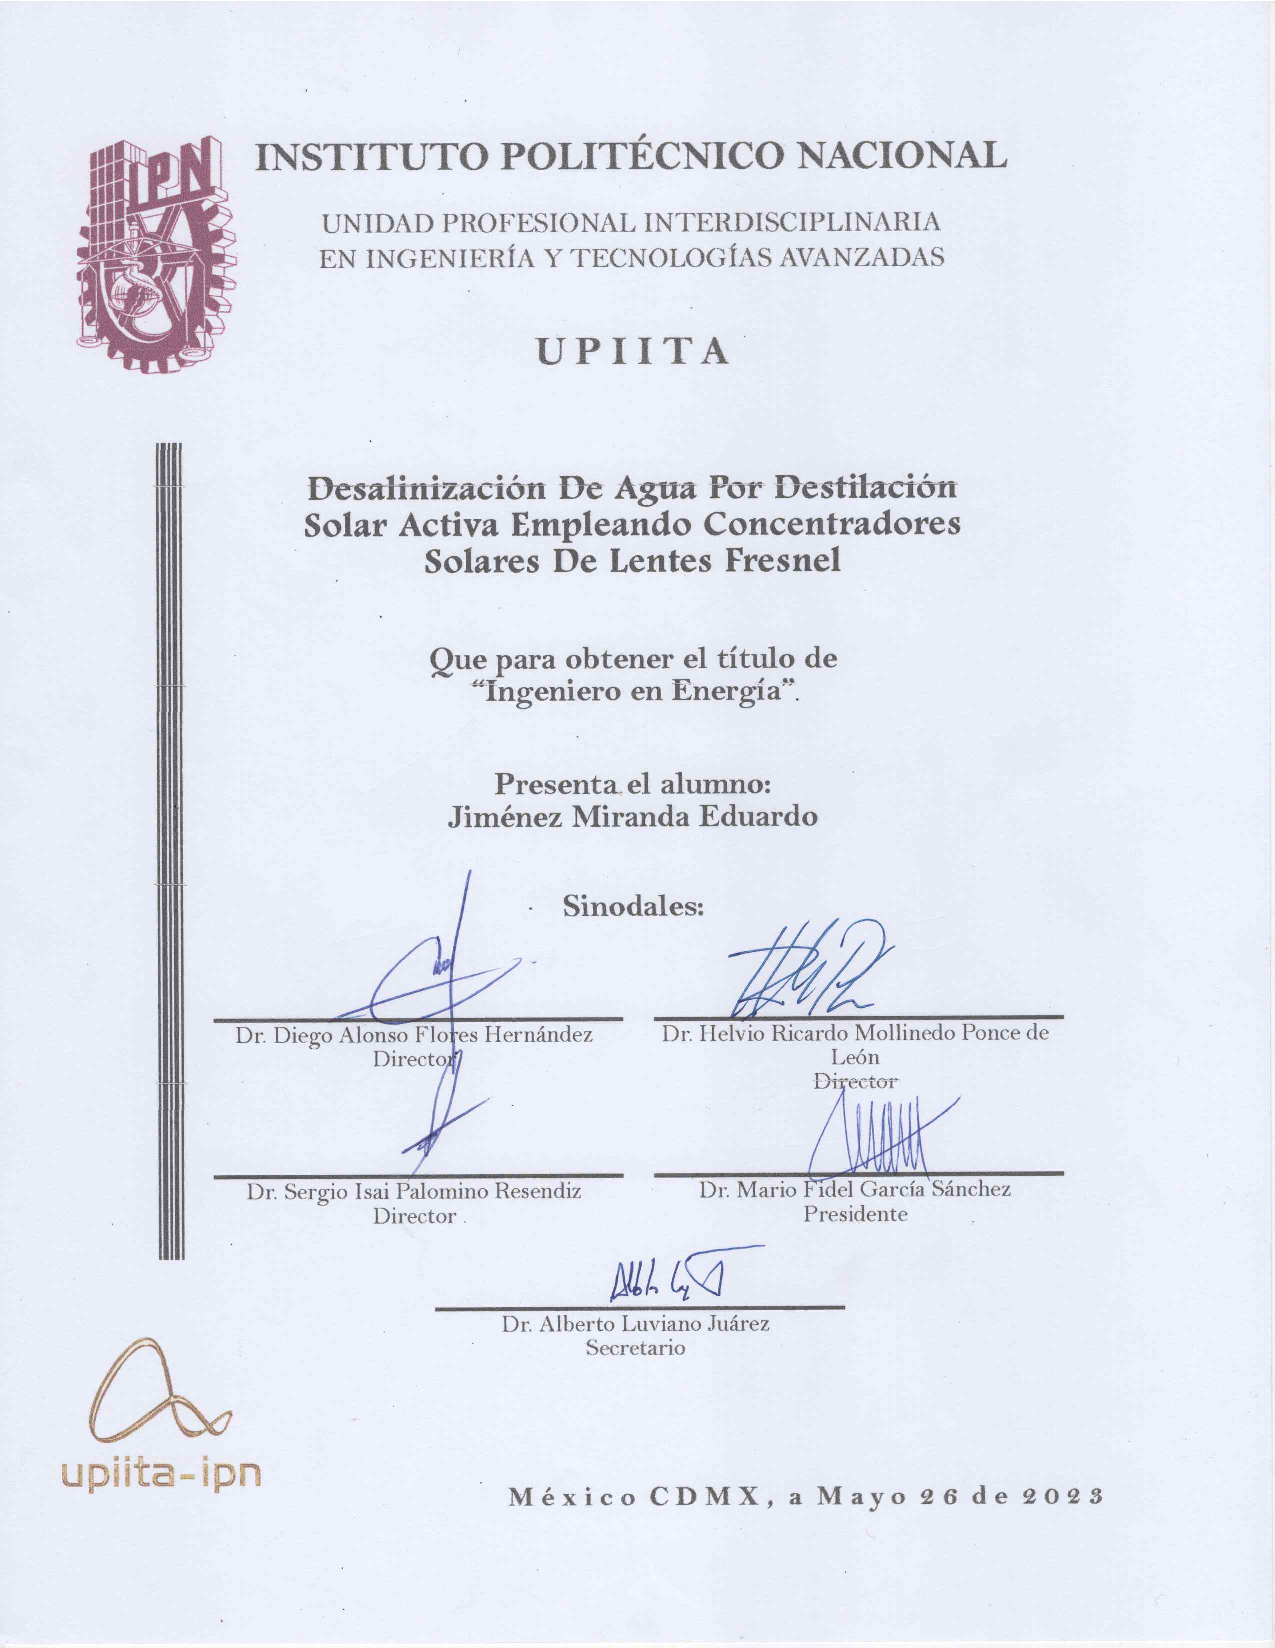
\includepdf{Content/Firmas.pdf}
	\begingroup
\BellMT

\tikzexternaldisable
\begin{tikzpicture}[remember picture,overlay,shorten >= -10pt]

	\coordinate (top) at ([yshift=-20mm]current page.north);
	\coordinate (top-right) at ([xshift=-25mm, yshift=-20mm]current page.north east);
	\coordinate (bottom-right) at ([xshift=-25mm, yshift=20mm]current page.south east);
	\coordinate (top-left) at ([xshift=25mm, yshift=-20mm]current page.north west);
	\coordinate (bottom-left) at ([xshift=25mm, yshift=20mm]current page.south west);
	
	% Líneas de decoración
	\begin{scope}[black]
		\foreach \x in {0, ..., 4}{
			\draw[line width=isodd(\x) ? 2pt : 1pt]([
					xshift=\x mm,
					yshift=-55mm
				]top-left)
				-- 
				([
					xshift=\x mm,
					yshift=45.7mm]
			bottom-left);
		};		
	\end{scope}
	% Logos
	\begin{scope}
		\node [anchor=north] (label) at (top-left) {
			
\includegraphics[
				width = 31.3mm,
				height = 41.5mm,
				keepaspectratio
			]{logos/IPN.png}
		};
		\node [anchor=south] (label) at (bottom-left) {
			
\includegraphics[
				width = 34.4mm,
				height = 32.2mm,
				keepaspectratio
			]{logos/UPIITA.png}
		};
	\end{scope}
	% Texto
	\begin{scope}
		\node [anchor=north] (IPN) at (top) {
			\fontsize{20pt}{20pt}\selectfont
			\bfseries
			INSTITUTO POLITÉCNICO NACIONAL
		};
		\node [below of = IPN, anchor = north, yshift=0.2em] (UNIDAD) {
			\fontsize{14pt}{14pt}\selectfont
			\parbox{\linewidth} {
				\centering
				UNIDAD PROFESIONAL INTERDISCIPLINARIA\\[0.25em]
				EN INGENIERÍA Y TECNOLOGÍAS AVANZADAS
			}
		};
		\node [below of = UNIDAD, anchor = north, yshift=-1.3em] (UPIITA) {
			\fontsize{20pt}{20pt}\selectfont
			\addfontfeature{LetterSpace=25}
			\bfseries
			UPIITA
		};
		
		\node [below of = UPIITA, anchor = north, yshift=-10mm] (Title) {
			\fontsize{18pt}{18pt}\selectfont
			\Footlight
			\parbox{0.7\linewidth} {
				\bfseries\centering
				\printtitle
			}
		};
		
		\node [below of = Title, anchor = north, yshift=-10mm] (Degree) {
			\fontsize{16pt}{16pt}\selectfont
			\parbox{0.7\linewidth} {
				\bfseries
				\centering
				Que para obtener el título de\\
				``Ingeniero en Energía''
			}
		};
		
		\node [below of = Degree, anchor = north, yshift=-5mm] (Students) {
			\fontsize{16pt}{16pt}\selectfont
			\parbox{0.7\linewidth} {
				\bfseries
				\centering
				Presenta el alumno:\\
				\printauthor
			}
		};
		
		\node [below of = Students, anchor = north, yshift=-5mm] (Advisors) {
			\fontsize{16pt}{16pt}\selectfont
			\parbox{0.7\linewidth} {
				\bfseries
				\centering
				Sinodales:
			}
		};
		
		\matrix [
			column sep=5mm,
			below of = Advisors,
			yshift=-32mm,
			matrix of nodes,
			nodes={minimum width=7cm, minimum height=1cm},
			row sep= 2mm
		] {
			\node [
				anchor = north,
				path picture={
					\draw [ultra thick] (0, 0) -- ++(7cm, 0);
				},
				left=2mm
			] {
				\fontsize{12pt}{12pt}\selectfont
				\parbox{7cm} {
					\centering
					\vspace*{32pt}
					Dr. Diego Alonso Flores Hernández\\
					Director
				}
			};
			\node [
				anchor = north,
				path picture={
					\draw [ultra thick] (0, 0) -- ++(7cm, 0);
				},
				right=2mm
			] {
				\fontsize{12pt}{12pt}\selectfont
				\parbox{7cm} {
					\centering
					\vspace*{44pt}
					Dr. Helvio Ricardo Mollinedo Ponce de León\\
					Director
				}
			};\\
			\node [
				anchor = north,
				path picture={
					\draw [ultra thick] (0, 0) -- ++(7cm, 0);
				},
				left=2mm
			] {
				\fontsize{12pt}{12pt}\selectfont
				\parbox{7cm} {
					\centering
					\vspace*{32pt}
					Dr. Sergio Isai Palomino Resendiz\\
					Director
				}
			};
			\node [
				anchor = north,
				path picture={
					\draw [ultra thick] (0, 0) -- ++(7cm, 0);
				},
				right=2mm
			] {
				\fontsize{12pt}{12pt}\selectfont
				\parbox{7cm} {
					\centering
					\vspace*{32pt}
					Dr. Mario Fidel García Sánchez\\
					Presidente
				}
			};\\
			\node [
				anchor = north,
				path picture={
					\draw [ultra thick] (0, 0) -- ++(7.5cm, 0);
				}
			] {
				\fontsize{12pt}{12pt}\selectfont
				\parbox{7.5cm} {
					\centering
					\vspace*{32pt}
					M. en C. Joaquin Alfredo Velazquez Olvera\\
					Secretario
				}
			};\\
		};
		
		\node [anchor=east] (Date) at (bottom-right) {
			\fontsize{14pt}{14pt}\selectfont
			\addfontfeature{LetterSpace=25}
			\bfseries
			México CDMX, a Diciembre 15 de 2023
		};
	\end{scope}
\end{tikzpicture}
\tikzexternalize
\endgroup
	\clearpage\newpage
	\chapter*{Agradecimientos}
	
	\vspace*{5mm}
	
	El Instituto Politécnico Nacional me ha dado grandes oportunidades para desarrollarme como persona y como profesionista, dando el espacio y permitiendo que conociera a gente maravillosa que ha dejado huella en mi vida; por eso mismo quiero expresar mi agradecimiento a mi institución que tantas herramientas me ha dado, así mismo, dedico este espacio para reconocer el apoyo y el conocimiento que me ha brindado la Unidad Profesional Interdisciplinaria en Ingeniería y Tecnologías Avanzadas y el Centro de Estudios Científicos y Tecnológicos No. 9 ``Juan De Dios Bátiz''.
	
	Le agradezco enormemente a mi familia quien me ha dado su apoyo incondicional y me ha dado la posibilidad de cursar una carrera universitaria, dándome las herramientas para crecer como una persona de bien y dejándome sin palabras para expresar mi gratitud hacia ellos.
	
	A mis directores quienes me han orientado y guiado durante la elaboración de este proyecto quiero agradecerles por el acompañamiento y el conocimiento que me han brindado.
	
	\clearpage\newpage	
	\tableofcontents
	\listoffigures
	\listoftables

	\clearpage\newpage
	\pagenumbering{Roman}	
	\glsfindwidesttoplevelname[\acronymtype]
	\printglossary[
		style=custommcolalttree,
		type=\acronymtype,
		title=Abreviaciones y acrónimos
	]
	
	\clearpage\newpage
	\printglossary[
		style=symbolunittable,
		title=Simbología,
		type=csymbols
	]
	\clearpage\newpage
	
	\begin{abstract}
	\addcontentsline{toc}{section}{Resumen}
	
	\noindent El siguiente trabajo desarrolla una propuesta técnica para la desalinización térmica de agua de mar por \gls{destilacion_solar} activa mediante el uso de lentes Fresnel como concentradores solares. Se identificaron algunos problemas asociados con base en la revisión de trabajos previos y conocimiento técnico del propio método; se planteó un diseño buscando mitigar los efectos de la intermitencia del Sol y la condensación del agua sobre la superficie de vidrio de los diseños más comunes. Para ello se estableció una serie de análisis térmicos, ópticos y estructurales que desembocaron en el diseño de una serie de módulos acoplados verticalmente.
	
	\noindent El propósito de este proyecto es coadyuvar al derecho de acceso al agua limpia a un precio asequible siendo el fin último contribuir al objetivo de desarrollo sostenible 6.a. a través de fuentes de energía sostenibles.
	
	\keywords{desalinización térmica, concentradores solares, destilación solar activa, lentes de Fresnel}
\end{abstract}

\bgroup
	\selectlanguage{english}
	\begin{abstract}
		\noindent This work bears a technical proposal for thermal desalination of seawater by active solar distillation through Fresnel solar concentrators. Some associated problems were identified based on the review of previous works and technical knowledge of the method itself; a design was proposed to mitigate the effects of the intermittence of the Sun and water condensation on the glass surface presented by the common designs. To this end, a series of thermal, optical and structural analyses was established that led to the design of a series of vertically coupled modules.
				
		\noindent This project seeks to assist the right of access to clean water at an affordable price, being the ultimate goal to contribute to the sustainable development goal 6.a. using sustainable energy sources.
		
		
		\keywords[Index terms]{thermal desalination, solar concentrators, active solar distillation, fresnel lenses}
	\end{abstract}
\egroup
	\glsfindwidesttoplevelname[\glsdefaulttype]
	\printglossary[style=alttree]
	
	\cleardoublepage
	\pagenumbering{arabic}
	%%%
	% Contenido
	%%%
	\input{Content/Chapter-1/Introducción.tex}
	\chapter{Objetivos}
	\section{Objetivo General}
		Diseñar y construir un destilador solar activo usando concentradores solares de lentes de fresnel para destilar agua salada
	\section{Objetivos específicos}
		\begin{enumerate}[I]
			\item Diseñar los sistemas de tuberías y almacenamiento donde fluirá y reposará el agua salada.
			\item Diseñar el concentrador solar y el mecanismo con el que se integrará al sistema de tuberías.
			\item Estudiar los modelos térmicos que caractericen o aproximen el comportamiento del concentrador solar y del proceso de evaporación.
			\item Definir los parámetros asociados a la desalinización con los que operará el sistema tales como la taza volumétrica de agua o la salinidad del agua de alimentación.
			\item Analizar los datos ambientales de temperatura e irradiación solar de la Ciudad de México para tener información climática sobre el lugar donde se desarrollará el proyecto.
			\item Construir los componentes que integran al destilador solar con base en los diseños propuestos.
			\item Desarrollar el mecanismo de control para regular la velocidad de flujo del agua mediante la implementación de programación y sistemas de control.
			\item Integrar a un seguidor solar el concentrador para mejorar la captación de calor.
			\item Evaluar el desempeño del destilador solar con base en el agua de salida para verificar la viabilidad del mismo.
			\end{enumerate}
	\chapter{Planteamiento del problema}

	Globalmente existen más de \num{18000} plantas desalinizadoras que contribuyen a garantizar el derecho de acceso a agua limpia y saneamiento a millones de personas. De acuerdo a las distintas condiciones como lo son el clima, la geografía, la política y la accesibilidad tecnológica, se selecciona el método de desalinización más adecuado, entre ellos, la ósmosis inversa se ha convertido en la tecnología más popular a nivel industrial \cite[11]{lattemann_chapter_2010} y se prevé que siga aumentando su presencia \cite{intelligence_ro_2021} debido a que es un proceso de alto rendimiento y económicamente favorable en relación al costo por litro de agua producido.
	
	Aunque esta industria ha madurado rápidamente en los últimos 40 años, aún existen áreas de oportunidad en los procesos ya que en general, la desalinización se considera de alto consumo energético y de grandes costos de construcción y operación. Aunado a ello, se presentan varios retos ambientales que comprendes entre otros: la huella ecológica de su construcción, las emisiones de \acrshort{gei} productos de la operación, impactos asociados a la obtención del agua salada y la materia prima que se utilice y la disposición final de residuos. Siendo en ocasiones el último facto un criterio que define la viabilidad final de una planta \cite{singh_experimental_2016}.
	
	Dado lo anterior, la incorporación de estrategias para incorporar energía renovable a los procesos de desalinización y el desarrollo de las tecnologías disponibles para aumentar la eficiencia energética resulta en una tarea indispensable para cubrir sosteniblemente la creciente demanda de agua. Está claro que esta visión debe ser complementada por la concienciación de la población y la creación de políticas para un mejor manejo de los recursos hídricos disponibles.
	
	Con base en lo ya expuesto, este proyecto plantea el desarrollo de un destilador solar activo e híbrido capaz de desalinizar a un ritmo lo más constante posible de acuerdo a las condiciones climáticas y geológicas disponibles. Para ello, se plantean los siguientes retos de ingeniería específicos a resolver:
	
	\begin{itemize}
		\item Obtención y caracterización del agua salada a usarse como materia prima.
		\item Obtención y análisis de los datos ambientales del lugar de desarrollo para identificar las variables ambientales de interés que influirán en la operación del sistema propuesto.
		\item Diseño del sistema y elaboración del modelo térmico que lo regirá así como la implementación de estrategias para reducir las pérdidas e intensificar la transferencia de calor.
		\item Propuesta de la capacidad de desalinización del sistema y selección de las lentes de concentración de acuerdo a la potencia requerida.
		\item Monitoreo del sistema y regulación del flujo de agua.
		\item Construcción del sistema.
	\end{itemize}
	
%	analizar la implementación sostenible de destiladores solares activos en lugares de alta irradiación solar con fácil acceso a cuerpos acuosos salobres, pues es un lugar idóneo de aplicación donde esta tecnología consigue explotar a su favor las condiciones climáticas y geográficas.
%	
%	Para ello debemos superar diversos retos de ingeniería específicos a resolver, entre los que se encuentran:
	\input{Content/Chapter-4/Justificación.tex}
	\input{Content/Chapter-5/Marco-teórico.tex}
	\chapter{Desarrollo experimental}
	
	Este trabajo busca realizar una investigación cuasi-experimental para reportar el comportamiento  del destilador solar propuesto de acuerdo a la influencia de las variables independientes descritas en la~\cref{table:variables-independientes-desarrollo-experimental}.
	
	\begin{longtblr}[
		caption = {Variables del desarrollo experimental},
		label = {table:variables-independientes-desarrollo-experimental},
		note{*} = {Se puede ejercer control directo sobre esta variable.}
	]{
		colspec = {X[l] c c X[2, l]},
		hlines,
		vlines,
		row{odd} = {bg=tablerowblue},
		row{1} = {
			bg = tabletitleblue,
			fg=white,
			font = \bfseries,
			halign=c
		},
		rowhead = 1,
		rows={m}
	}
		Variable & Clasificación & Tipo de dato & Influencia en el modelo\\
		Temperatura de entrada del agua\TblrNote{*}
			& Independiente
			& Cuantitativa
			& Establece la temperatura inicial del modelo térmico para la ebullición del agua\\
		Presión atmosférica
			& Independiente
			& Cuantitativa
			& Modifica la temperatura a la cual sucede el cambio de fase del agua\\
		Temperatura ambiente
			& Independiente
			& Cuantitativa
			& Influye en las pérdidas de calor que tendrá el sistema\\
		Clima (nubosidad)
			& Independiente
			& Cualitativa
			& Punto de comparación rápido para ver la influencia de la nubosidad sobre el desempeño\\
		Velocidad de viento
			& Independiente
			& Cuantitativa
			& Se asocia directamente a las pérdidas de calor por convección\\
		Hola del día
			& Independiente
			& Cuantitativa
			& Determina la posición angular del Sol y se relaciona con la irradiación solar\\
		Irradiación solar promedio
			& Independiente
			& Cuantitativa
			& Determina la potencia solar recibida en nuestro modelo de transferencia de calor\\
		Temperatura de salida del agua
			& Dependiente
			& Cuantitativa
			& Asociada al cambio de fase del agua\\
		Temperatura del recibidor solar
			& Dependiente
			& Cuantitativa
			& Influye en los modelos térmicos para la destilación del agua\\
		Caudal de agua\TblrNote{*} 
			& Dependiente
			& Cuantitativa
			& Influye en los modelos térmicos y la tasa de desalinización\\
		Propiedades físico-químicas del agua
			& Dependiente
			& Cuantitativa
			& Indica la calidad del agua
	\end{longtblr}
	
	\section{Grupos de estudio}
		
		Con base en las variables observadas en la~\cref{table:variables-independientes-desarrollo-experimental} se distinguieron los grupos de control descritos en las sub-secciones siguientes.
		
		\subsection{Agua}
			
			Las muestras de agua se seleccionaron guiándose en la~\cref{table:clasificacion-agua-tds}. Para ello, la obtención de agua de mar se simula con sales marinas para acuario y se proponen 3 grupos de control descritos en la~\cref{table:grupo-control-agua} para evaluar los casos límite y promedio de la salinidad del agua de mar.
			
			\begin{longtblr}[
				caption = {Grupo de control del agua de mar},
				label = {table:grupo-control-agua}
			]{
				colspec = {X[c] X[2, c]},
				hlines,
				vlines,
				width = 0.5\linewidth,
				rowhead = 1,
				row{odd} = {bg=tablerowblue},
				row{1} = {
					bg = tabletitleblue,
					fg=white,
					font = \bfseries,
					halign=c
				},
				rows={m}
			}
				Muestra & Salinidad (\unit{\mg\per\litre})\\
				1 & \num{30000}\\
				2 & \num{35000}\\
				3 & \num{40000}
			\end{longtblr}
		
		\subsection{Lugar físico de experimentación}\label{sec:ch6-lugar-fisico}
			
			Debido al alcance del proyecto, se acotó el lugar físico de experimentación a la Unidad Profesional Interdisciplinaria en Ingeniería y Tecnologías Avanzadas ubicada en la Ciudad de México.
			
			\begin{longtblr}[
				caption = {Grupo de control del agua de mar},
				label = {table:grupo-control-fisico}
			]{
				colspec = {X[c] *{3}{c}},
				hlines,
				vlines,
				width = 0.8\linewidth,
				rowhead = 1,
				row{odd} = {bg=tablerowblue},
				row{1} = {
					bg = tabletitleblue,
					fg=white,
					font = \bfseries,
					halign=c
				},
				rows={m}
			}
				Zona & Longitud & Latitud & Altitud\\
				Ciudad de México, México
					& \ang{-99;07;32}
					& \ang{19;30;38}
					& \qty{2241}{\m}
			\end{longtblr}
			
			\subsubsection{Variables climáticas sobre la región a investigar}
				
				Debido a la naturaleza de nuestra fuente de energía y que su operación no transcurren dentro de un ambiente controlado se deben evaluar las condiciones climáticas del lugar que impactan en mayor medida el sistema propuesto.
				
				\begin{longtblr}[
					caption = {Variables climáticas consideradas importantes para la investigación},
					label = {table:variables-climaticas},
					note{?} = {Se decidió incluir en el estudio a esta variable dado a que no se sabe con certeza si será necesaria para el futuro desarrollo.}
				]{
					colspec = {X[c] X[3, l] c},
					hlines,
					vlines,
					width = \linewidth,
					row{odd} = {bg=tablerowblue},
					rowhead = 1,
					row{1} = {
						bg = tabletitleblue,
						fg=white,
						font = \bfseries,
						halign=c
					},
					rows={m}
				}
					Variable & Descripción & Unidades\\
					Presión superficial
						& Presión promedio en la superficie del lugar
						& \unit{\kilo\pascal}\\
					Velocidad de viento
						& Velocidad de viento promedio a 2 metros sobre la superficie del lugar
						& \unit{\m\per\s}\\
					Humedad específica
						& Razón promedio de la masa de vapor de agua por unidad de aire a 2 metros sobre la superficie del lugar
						& \unit{\gram\per\kg}\\
					\acrfull{roc} sobre cielo despejado
						& Total de irradiación solar incidida (directa más difusa) sobre la tierra en un plano horizontal sobre la superficie de la tierra a condiciones de cielo despejado.
						& \unit{\watt\hour\per\m\tothe{2}}\\
					\acrlong{roc}
						& Total de irradiación solar incidida (directa más difusa) sobre la tierra en un plano horizontal sobre la superficie de la tierra a todas las condiciones.
						& \unit{\watt\hour\per\m\tothe{2}}\\
					Nubosidad
						& Porcentaje promedio de cantidad de nubes en el cielo sobre un lapso determinado
						& \unit{\watt\hour\per\m\tothe{2}}\\
					Irradiancia UVA\TblrNote{?}
						& Radiación UVA (\qtyrange{315}{400}{\nm}) total incidida a todas las condiciones climáticas del día
						& \unit{\watt\per\m\tothe{2}}\\
					Irradiancia UVB\TblrNote{?}
						& Radiación UVB (\qtyrange{280}{315}{\nm}) total incidida a todas las condiciones climáticas del día
						& \unit{\watt\per\m\tothe{2}}	
				\end{longtblr}

	\section{Descripción de los problemas asociados a la destilación solar}
		
		Gracias a una entrevista informal con el Dr. Palomino acerca del modelo propuesto en \cite{palomino-resendiz_design_2018}, se identificó que la humedad suele condensarse sobre el vidrio o cristal afectando así la transmisividad y por ende el calor efectivo que llega al agua. Además, debido a la naturaleza intermitente de la energía solar, el proceso de desalinización suele presentar caídas grandes de producción en presencia de una nube.
		
		Por ello, este diseño se encaminó a mitigar en lo posible los problemas identificados proponiendo un método de almacenamiento de energía térmica y transferencia indirecta de calor.
		
	\section{Configuración experimental}
		
		Para definir los criterios de operación sobre los cuales se espera que opere en pruebas el sistema, se realizó un análisis de datos de las variables climáticas propuestas. Los datos utilizados fueron obtenidos de \textit{NASA Langley Research Center (LaRC) POWER Project} financiado por el Programa de Ciencias de la Tierra/Ciencias Aplicadas de la NASA usando el código mostrado en el \cref{ch:solar-irradiation-code}.
		
		De dicho código se obtuvieron gráficas de área que nos representaban el comportamiento reportado por \textit{The Power LaRC} en intervalos de cada hora.
	
		\subsection{Radiación solar de onda corta}
			
			En la~\cref{fig:SFC_SW_DWN} observamos que de marzo a septiembre tenemos los niveles más altos de \acrlong{roc} y esta radiación se encuentra dentro de un rango de \qtyrange{5}{8}{\kWh\per\m\tothe{2}\day}.
			
			De la~\cref{fig:ALLSKY_SFC_SW_DWN_surface_2020_3d} se observa que la irradiancia se de \acrshort{roc} de interés varía entre los \qtyrange{500}{900}{\watt\per\m\tothe{2}} y se aprecia que en mayor proporción se encuentra entre \qtyrange{600}{700}{\watt\per\m\tothe{2}} por lo que para los cálculos de operación se decide usar \qty{650}{\watt\per\m\tothe{2}} como valor de irradiancia.
	
			\begin{figure}[H]
				\centering
				\begin{subfigure}[t]{0.45\linewidth}
					\centering
					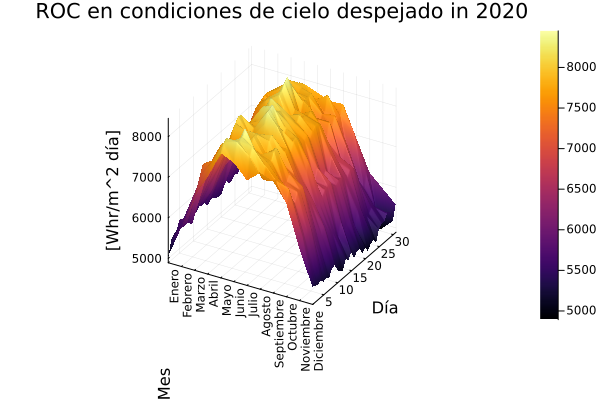
\includegraphics[
						width=\linewidth,
						height = 60mm,
						keepaspectratio
					]{Resultados/DataAnalysis/CLRSKY_SFC_SW_DWN_surface_2020_3d.png}
					\caption{Irradiación de onda corta total recibida por día en condiciones de cielo despejado durante el 2020 sobre el lugar seleccionado}
					\label{fig:CLRSKY_SFC_SW_DWN_surface_2020_3d}
				\end{subfigure}
				\hfill
				\begin{subfigure}[t]{0.45\linewidth}
					\centering
					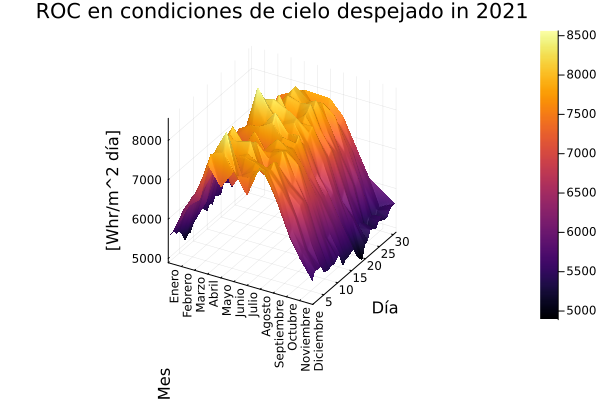
\includegraphics[
						width=\linewidth,
						height = 60mm,
						keepaspectratio
					]{Resultados/DataAnalysis/CLRSKY_SFC_SW_DWN_surface_2021_3d.png}
					\caption{Irradiación de onda corta total recibida por día en condiciones de cielo despejado durante el 2021 sobre el lugar seleccionado}
					\label{fig:CLRSKY_SFC_SW_DWN_surface_2021_3d}
				\end{subfigure}
			\end{figure}
			
			\begin{figure}[H]\ContinuedFloat
				\begin{subfigure}[t]{0.45\linewidth}
					\centering
					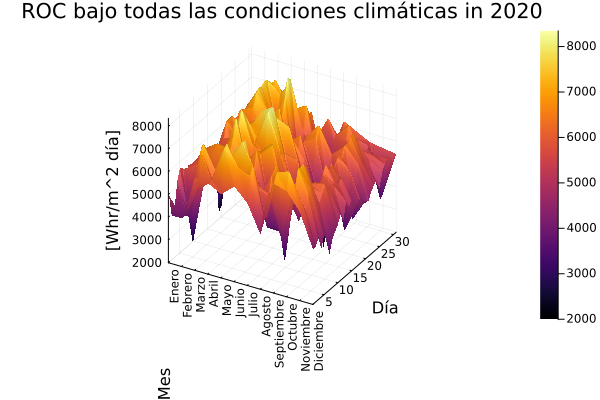
\includegraphics[
						width=\linewidth,
						height = 60mm,
						keepaspectratio
					]{Resultados/DataAnalysis/ALLSKY_SFC_SW_DWN_surface_2020_3d.png}
					\caption{Irradiación de onda corta total recibida por día bajo todas las condiciones climáticas durante el 2020 sobre el lugar seleccionado}
					\label{fig:ALLSKY_SFC_SW_DWN_surface_2020_3d}
				\end{subfigure}
				\hfill
				\begin{subfigure}[t]{0.45\linewidth}
					\centering
					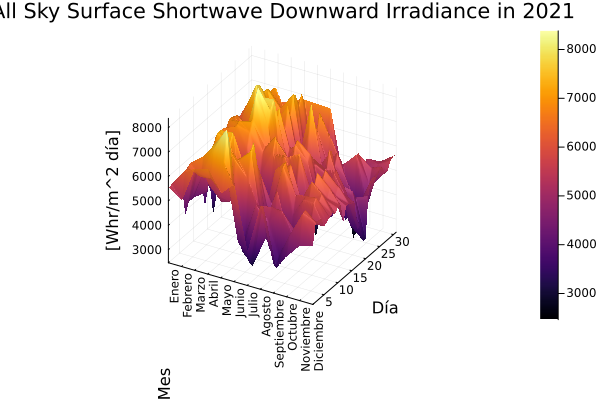
\includegraphics[
						width=\linewidth,
						height = 60mm,
						keepaspectratio
					]{Resultados/DataAnalysis/ALLSKY_SFC_SW_DWN_surface_2021_3d.png}
					\caption{Irradiación de onda corta total recibida por día bajo todas las condiciones climáticas durante el 2021 sobre el lugar seleccionado}
					\label{fig:ALLSKY_SFC_SW_DWN_surface_2021_3d}
				\end{subfigure}
			\end{figure}
			
			\begin{figure}[H]\ContinuedFloat
				\begin{subfigure}[t]{0.45\linewidth}
					\centering
					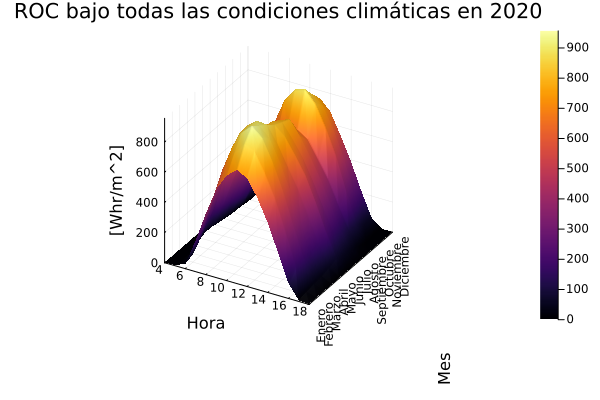
\includegraphics[
						width=\linewidth,
						height = 60mm,
						keepaspectratio
					]{Resultados/DataAnalysis/ALLSKY_SFC_SW_DWN_3d_mean_2020.png}
					\caption{Irradiación de onda corta promedio recibida por hora bajo todas las condiciones climáticas durante el 2020 sobre el lugar seleccionado}
					\label{fig:ALLSKY_SFC_SW_DWN_3d_mean_2020}
				\end{subfigure}
				\hfill
				\begin{subfigure}[t]{0.45\linewidth}
					\centering
					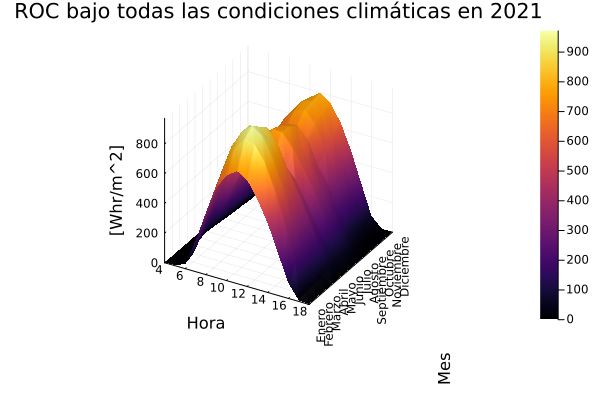
\includegraphics[
						width=\linewidth,
						height = 60mm,
						keepaspectratio
					]{Resultados/DataAnalysis/ALLSKY_SFC_SW_DWN_3d_mean_2021.png}
					\caption{Irradiación de onda corta promedio recibida por hora bajo todas las condiciones climáticas durante el 2021 sobre el lugar seleccionado}
					\label{fig:ALLSKY_SFC_SW_DWN_3d_mean_2021}
				\end{subfigure}
				\caption{Irradiación de onda corta recibida en el lugar físico de experimentación durante 2020 y 2021}
				\label{fig:SFC_SW_DWN}
			\end{figure}

		\subsection{Temperatura}
			
			Debido a que no se pudo obtener una base de datos que proporcionara la temperatura en intervalos de una hora, se decidió usar el resumen presentado por WeatherSpark, el cual se puede observar en la~\cref{fig:Temperatura-CDMX}.
			
			De la revisión de la~\cref{fig:Temperatura-CDMX} se observa que la temperatura mínima durante los meses de mayor radiación solar se tiene una temperatura mínima de \qty{13}{\degreeCelsius} y se define que la temperatura inicial del agua de entrada sería cercana a los \qty{15.5}{\degreeCelsius}. Para condiciones de operación en horas más avanzadas, el agua de entrada se encontraría entre los \qtyrange{18}{24}{\degreeCelsius}.
			
			\begin{figure}[H]
				\centering
				\begin{subfigure}[t]{\linewidth}
					\centering
					\includegraphics[
						width=\linewidth,
						height=70mm,
						keepaspectratio
					]{Resultados/DataAnalysis/Temperatura-promedio-por-hora-en-Ciudad-de-México.png}
					\\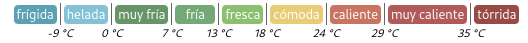
\includegraphics[
						width=0.8\linewidth,
						keepaspectratio
					]{Resultados/DataAnalysis/WeatherSpark-Temperatura-Leyenda.png}
					\caption{Temperatura promedio por hora en Ciudad de México}
					\label{fig:Temperatura-promedio-por-hora-en-Ciudad-de-México}
				\end{subfigure}
			\end{figure}
			\begin{figure}[H]\ContinuedFloat
				\begin{subfigure}[t]{\linewidth}
					\centering
					\includegraphics[
						width=\linewidth,
						height=70mm,
						keepaspectratio
					]{Resultados/DataAnalysis/Temperatura-por-hora-en-2022-Ciudad-de-México.png}\\
					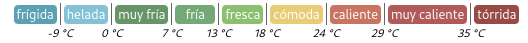
\includegraphics[
						width=0.8\linewidth,
						keepaspectratio
					]{Resultados/DataAnalysis/WeatherSpark-Temperatura-Leyenda.png}
					\caption{Temperatura por hora del 2022 en la Ciudad de México}
					\label{fig:Temperatura-por-hora-en-2022-Ciudad-de-México}
				\end{subfigure}
				\caption{Mapas de temperaturas de la Ciudad de México}
				\floatfoot{Los gráficos fueron obtenidos de \href{https://es.weatherspark.com/y/5674/Clima-promedio-en-Ciudad-de-México-México-durante-todo-el-año}{\textcopyright WeatherSpark.com}}
				\label{fig:Temperatura-CDMX}
			\end{figure}
		
		\subsection{Presión atmosférica}
			
			En la~\cref{fig:PS_3d_mean} se observa que la presión superficial varía muy poco, debido a ello sólo se tomará el valor redondeado de \qty{75}{\kilo\pascal} para cálculos posteriores.
			
			\begin{figure}[H]
				\centering
				\begin{subfigure}[t]{0.45\linewidth}
					\centering
					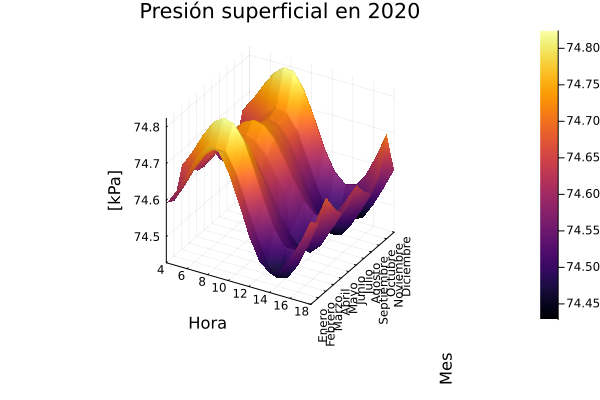
\includegraphics[
						width=\linewidth,
						height = 60mm,
						keepaspectratio
					]{Resultados/DataAnalysis/PS_3d_mean_2020.png}
					\caption{Presión promedio por hora del viento durante 2020 sobre el lugar seleccionado}
					\label{fig:PS_3d_mean_2020}
				\end{subfigure}
				\hfill
				\begin{subfigure}[t]{0.45\linewidth}
					\centering
					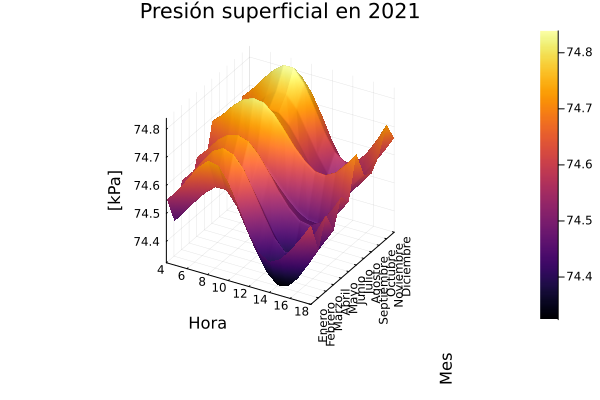
\includegraphics[
						width=\linewidth,
						height = 60mm,
						keepaspectratio
					]{Resultados/DataAnalysis/PS_3d_mean_2021.png}
					\caption{Presión promedio por hora del viento durante 2021 sobre el lugar seleccionado}
					\label{fig:PS_3d_mean_2021}
				\end{subfigure}
				\caption{Presión promedio en el lugar físico de experimentación durante 2020 y 2021}
				\label{fig:PS_3d_mean}
			\end{figure}
			
		\subsection{Magnitud del perfil de velocidad del viento}
		
			Debido a las pérdidas térmicas esperadas por convección forzada se estudió este criterio, sin embargo, como se observa en la~\cref{fig:WS2M_3d_mean} no se distingue visiblemente un patrón en el comportamiento. Se decidió usar un valor promedio de \qty{1.5}{\m\per\s}.
			
			\begin{figure}[H]
				\centering
				\begin{subfigure}[t]{0.45\linewidth}
					\centering
					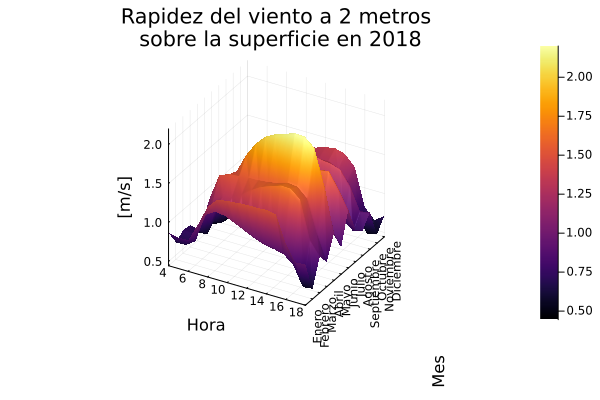
\includegraphics[
						width=\linewidth,
						height = 60mm,
						keepaspectratio
					]{Resultados/DataAnalysis/WS2M_3d_mean_2018.png}
					\caption{Rapidez promedio por hora del viento durante 2018 sobre el lugar seleccionado}
					\label{fig:WS2M_3d_mean_2018}
				\end{subfigure}
				\hfill
				\begin{subfigure}[t]{0.45\linewidth}
					\centering
					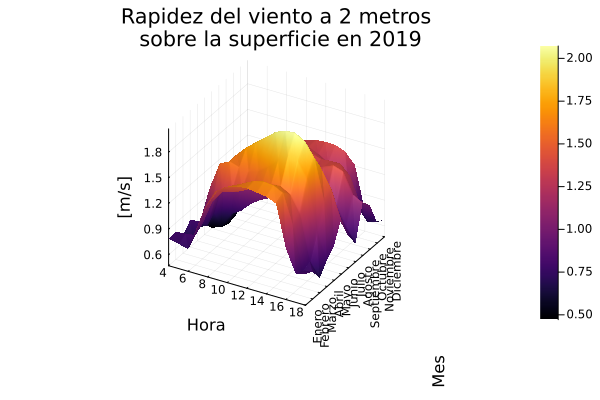
\includegraphics[
						width=\linewidth,
						height = 60mm,
						keepaspectratio
					]{Resultados/DataAnalysis/WS2M_3d_mean_2019.png}
					\caption{Rapidez promedio por hora del viento durante 2019 sobre el lugar seleccionado}
					\label{fig:WS2M_3d_mean_2019}
				\end{subfigure}
			\end{figure}
			
			\begin{figure}[H]\ContinuedFloat
				\begin{subfigure}[t]{0.45\linewidth}
					\centering
					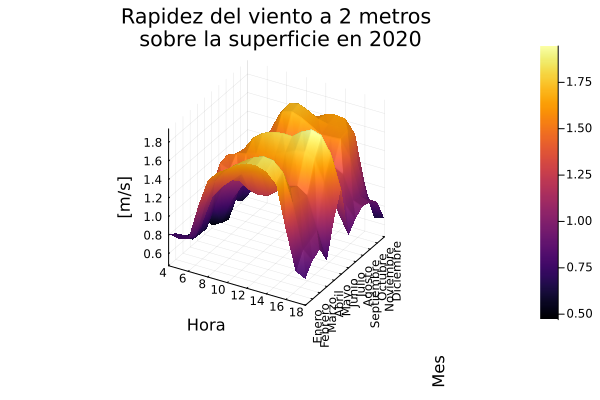
\includegraphics[
						width=\linewidth,
						height = 60mm,
						keepaspectratio
					]{Resultados/DataAnalysis/WS2M_3d_mean_2020.png}
					\caption{Rapidez promedio por hora del viento durante 2020 sobre el lugar seleccionado}
					\label{fig:WS2M_3d_mean_2020}
				\end{subfigure}
				\hfill
				\begin{subfigure}[t]{0.45\linewidth}
					\centering
					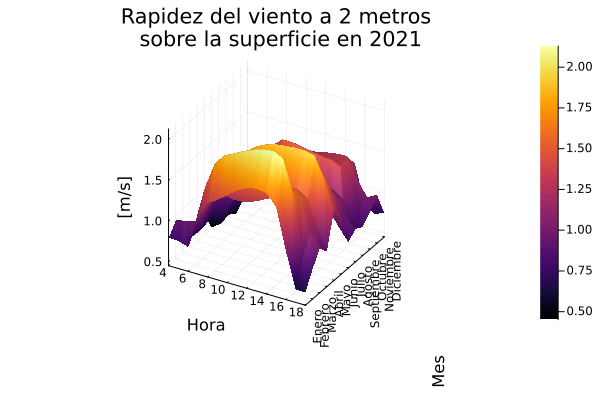
\includegraphics[
						width=\linewidth,
						height = 60mm,
						keepaspectratio
					]{Resultados/DataAnalysis/WS2M_3d_mean_2021.png}
					\caption{Rapidez promedio del viento durante 2021 sobre el lugar seleccionado}
					\label{fig:WS2M_3d_mean_2021}
				\end{subfigure}
				\caption{Rapidez promedio por hora del viento sobre el lugar seleccionado}
				\label{fig:WS2M_3d_mean}
			\end{figure}
	
		\subsection{Definición de valores esperados de la configuración experimental}
			
			Usando los límites de operación encontrados del análisis de datos se calcula mediante \eqref{equ:interpolación-lineal-simple} y los datos de los~\cref{ch:seawater-properties,ch:agua-saturada-propiedades} la temperatura de ebullición del agua de mar en el sitio de experimentación y a la cual se le agrega un \percent{2} de tolerancia.
			
			\begin{equation}\label{equ:interpolación-lineal-simple}
				y = y_{0} + \dfrac{y_{1}-y_{0}}{x_{1}-x_{0}} \times (x-x_{0})
			\end{equation}
			
			\begin{longtblr}[
				caption = {Datos a interpolar para definir los parámetros de salida del agua},
				label = {table:interpolación-agua-salida},
			]{
				colspec = {*{3}{X}},
				hlines,
				vlines,
				row{odd} = {bg=tablerowblue},
				row{1} = {
					bg = tabletitleblue,
					fg=white,
					font = \bfseries
				},
				width=0.75\linewidth,
				rowhead = 1,
				rows={
					valign = m,
					halign = c,
					mode = math
				}
			}
				~ & y & x\\
				0 & \qty{90}{\degreeCelsius} & \qty{70.14}{\kilo\pascal}\\
				1 & \qty{95}{\degreeCelsius} & \qty{80.55}{\kilo\pascal}\\
				\text{T}_{\text{salida}} & ~ & \qty{74.80}{\kilo\pascal}
			\end{longtblr}
			
			\begin{align*}
				\text{T}_{\text{ebullición agua dulce}} &= \qty{90}{\degreeCelsius} + \dfrac{\qty{95}{\degreeCelsius} - \qty{90}{\degreeCelsius}}{\qty{80.55}{\kilo\pascal}-\qty{70.14}{\kilo\pascal}} \times (\qty{74.80}{\kilo\pascal} - \qty{70.14}{\kilo\pascal})\\
				\text{T}_{\text{salida}} &= (\text{T}_{\text{ebullición agua dulce}} + \qty{0.601}{\degreeCelsius}) + \text{Tolerancia}\\
				\text{T}_{\text{salida}} &= (\qty{92.238}{\degreeCelsius} + \qty{0.601}{\degreeCelsius}) \times (1.02)\\
				\text{T}_{\text{salida}} &\approx \qty{94.70}{\degreeCelsius}
			\end{align*}
			
			Y considerando una temperatura de entrada del agua igual al inicio de sus operaciones de \qty{15.5}{\degreeCelsius} tenemos calculamos mediante \eqref{equ:potencia-necesaria-agua} el flujo de calor necesario por unidad de flujo másico que se necesita para lograr la ebullición del agua y el cambio de fase.
			
			\begin{equation}\label{equ:potencia-necesaria-agua}
				\dfrac{\dot{Q}}{\dot{m}} = \left(\gls{cs}_{\text{agua}} \Delta T + \gls{hl}\right)
			\end{equation}
			
			Para conocer $\gls{cs}_{\text{agua}}$ de la \cref{table:Calor-específico-agua} se usa \eqref{equ:interpolación-lineal-simple} para obtener el calor específico estimado a los \qty{13}{\degreeCelsius} y a los \qty{94.7}{\degreeCelsius}.
			
			\begin{align*}
				\gls{cs}_{13} &= \qty{3968.1}{\joule\per\kg\kelvin} + \dfrac{\qty{3973.4}{\joule\per\kg\kelvin} - \qty{3968.1}{\joule\per\kg\kelvin}}{\qty{20}{\degreeCelsius}-\qty{10}{\degreeCelsius}} \times (\qty{20}{\degreeCelsius} - \qty{13}{\degreeCelsius})\\
				\gls{cs}_{13} &= \qty{3971.8}{\joule\per\kg\kelvin}\\
				\gls{cs}_{94.7} &= \qty{4010.5}{\joule\per\kg\kelvin} + \dfrac{\qty{4019.9}{\joule\per\kg\kelvin} - \qty{4010.5}{\joule\per\kg\kelvin}}{\qty{100}{\degreeCelsius}-\qty{90}{\degreeCelsius}} \times (\qty{100}{\degreeCelsius} - \qty{94.7}{\degreeCelsius})\\
				\gls{cs}_{94.7} &= \qty{4015.5}{\joule\per\kg\kelvin}
			\end{align*}
			
			Una vez obtenidos sacamos el promedio incluyendo el resto del intervalo dándonos que:
			\begin{equation*}
				\gls{cs}_{\text{agua}} = \qty{3989.5}{\joule\per\kg\kelvin}
			\end{equation*}
			
			Similarmente para obtener \gls{hl} aplicamos \eqref{equ:interpolación-lineal-simple} en \cref{table:Calor-latente-vaporización} para obtener la entalpía de vaporización a los \qty{94.7}{\degreeCelsius}.
			
			\begin{align*}
				\gls{hl} &= \qty{2191.3}{\kilo\joule\per\kg} + \dfrac{\qty{2166.2}{\kilo\joule\per\kg} - \qty{2191.3}{\kilo\joule\per\kg}}{\qty{100}{\degreeCelsius}-\qty{90}{\degreeCelsius}} \times (\qty{100}{\degreeCelsius} - \qty{94.7}{\degreeCelsius})\\
				\gls{hl} &= \qty{2178.0}{\kilo\joule\per\kg}
			\end{align*}
			
			Sustituyendo en \eqref{equ:potencia-necesaria-agua} obtenemos que el flujo de calor necesario por unidad de flujo másico es:
			
			\begin{equation}\label{equ:potencia-necesaria-sistema}
				\dot{Q} = \dot{m}\left[\qty{3.9895}{\kilo\joule\per\kg\kelvin} \left(\qty{94.7}{\degreeCelsius}-\qty{15.5}{\degreeCelsius}\right) + \qty{2178.0}{\kilo\joule\per\kg}\right] = \dot{m} \times \qty{2493.97}{\kilo\joule\per\kg}
			\end{equation}
			
			
	\section{Planteamiento de la solución}
		\subsection{Selección y caracterización del elemento óptico de concentración}
			
			Para este proyecto son accesibles 4 modelos de lentes de Fresnel con ranuras hacia adentro cuyas características se ven resumidas en la~\cref{table:fresnel-lenses-models}.
			
			% Página 36
			\begin{longtblr}[
				caption = {Modelos y características de los concentradores solares},
				label = {table:fresnel-lenses-models}
			]{
				colspec = {*{2}{X[1.5]} *{2}{X} X[2.5] *{2}{X}},
				hlines,
				vlines,
				width = \linewidth,
				rowhead = 2,
				row{odd[3]} = {bg=tablerowblue},
				row{1,2} = {
					bg = tabletitleblue,
					fg=white,
					font = \bfseries,
					halign=c
				},
				rows={
					halign = c,
					valign = m
				}
			}
				Modelo & Longitud focal & Ancho & Largo & Material & Grosor & Tamaño de ranura\\
				--- & mm & mm & mm & --- & mm & mm\\
				CP220-280
					& \num{220}
					& \num{280}
					& \num{280}
					& PMMA: \acrshort{pvuvc}
					& \num{5}
					& \num{0.5}\\
				CP330-280
					& \num{330}
					& \num{280}
					& \num{280}
					& PMMA: \acrshort{pvuvc}
					& \num{5}
					& \num{0.5}\\
				CP350-300 
					& \num{350}
					& \num{310}
					& \num{310}
					& PMMA: \acrshort{pvuvc}
					& \num{5}
					& \num{0.5}\\
				CP350-330 
					& \num{350}
					& \num{340}
					& \num{340}
					& PMMA: \acrshort{pvuvc}
					& \num{5}
					& \num{0.5}
			\end{longtblr}
			
			Se halla en su hoja técnica que el PMMA \acrshort{pvuvc} tiene una transmitancia igual a \percent{92.65}.
			
			Para seleccionar la lente se tomaron como criterios el área de la lente y el número F (\gls{F}) dado por \eqref{equ:F-number}, ya que entre mayor sea \gls{F}, será mayor la capacidad de concentración y será mejor la capacidad de recolección de la lente.
			
			\begin{equation}\label{equ:F-number}
				\gls{F} = \dfrac{\gls{f}}{2\gls{Rl}}
			\end{equation}
			
			Conociendo eso, se determina que el modelo a usar es la lente de Fresnel condensadora \textbf{CP350-300} con un \gls{F} equivalente a \num{1.129}. 
			
			A continuación se enlistan algunas propiedades importantes del material seleccionado \cite{shannon_art_1997} citado por \cite{leutz_nonimaging_2001}.
			
			\begin{itemize}
				\item Índice de refracción: $\gls{nd} = 1.4918$
				\item Número de Abbe: $V_d = 54.7$
				\item Coeficiente de temperatura: $\sfrac{dn}{dT} \unit{\per\kelvin} = \num{-105e-6}$
			\end{itemize}
			
			\subsubsection{Ángulos para el trazado de rayos}
			
				Conociendo esto se calculan los ángulos $\alpha$, $\omega$ y $\beta$ necesarios para el cálculo en el trazado de rayos usando \cref{equ:rayos-alfa,equ:rayos-omega,equ:rayos-beta}. Donde $\alpha$ es la inclinación del prisma y $\beta$ es el ángulo del prisma.
				
				\begin{align}
					\tan\alpha &= \dfrac{R}{\gls{nd}\sqrt{R^{2}+f^{2}} - f} \label{equ:rayos-alfa}\\
					\tan\omega &= \dfrac{R}{f} \label{equ:rayos-omega}\\
					\tan\beta &= \alpha + \omega \label{equ:rayos-beta}
				\end{align}
				
				Lo que nos da: $\alpha= \ang{34.361}$, $\omega = \ang{22.989}$, $\beta= \ang{57.350}$
				
				Finalmente se describen las ecuaciones que se usan para modelar el trazado de rayos.
				
				\begin{align}
					\phi_{1} &= \beta - \alpha - \theta_{\text{entrada}}\\
					\phi_{1}\prime &= \arcsin\left(\dfrac{\sin\phi_{1}}{\gls{nd}\prime}\right)\\
					\phi_{t} &= \beta - \alpha - \phi_{1}\prime\\
					\phi_{2}\prime &= \phi_{t} + \alpha\\
					\phi_{2} &= \arcsin{\sin\phi_{2}\prime\gls{nd}\prime}\\
					\theta_{salida} &= \phi_{2} - \alpha
				\end{align}
				
			\subsubsection{Pérdidas por transmisión}
					
					Usando como referencia la~\cref{fig:Transmitancia} vemos que el elemento de concentración tiene una eficiencia de transmisión aproximada de \percent{83}. Además se propone el uso de cuarzo el cual tiene una eficiencia de transmisión de \percent{99.9} como ``ventana'' en la cámara del recibidor solar, asumiendo que el aire es un medio con $\gls{nd}_{\text{aire}} = 1$ y $\gls{tau}_{\text{aire}} = 1$, la transmisión total calculada del sistema esta dada por \eqref{equ:transmisión-cámara} mientras que la transmisión ideal esta dada por \cref{equ:transmisión-cámara-ideal}.
			
					\begin{figure}[H]
						\centering
						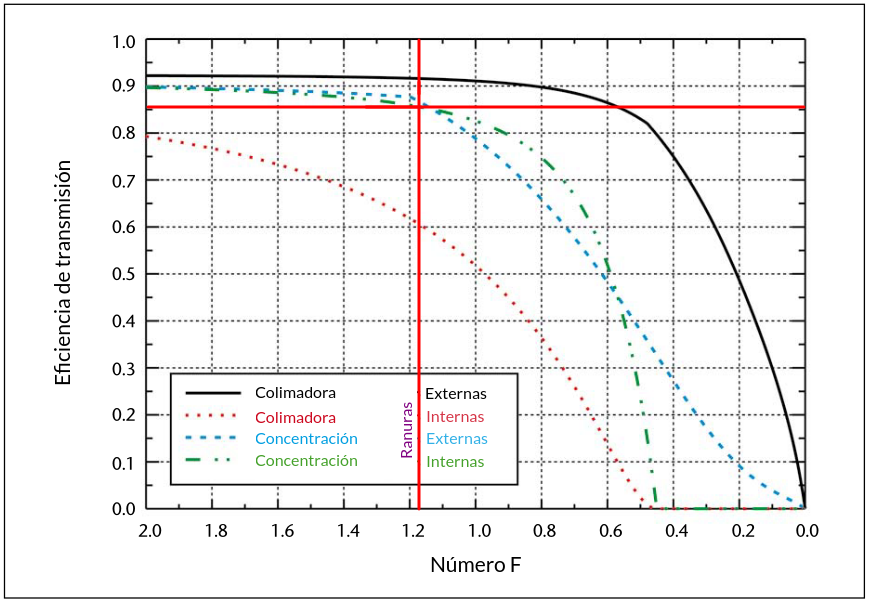
\includegraphics[
							width=\linewidth,
							height=85mm,
							keepaspectratio
						]{Desarrollo-experimental/Transmitancia.png}
						\caption{Valores de eficiencia idealizados de lentes de Fresnel calculadas en la reflexión de las superficies y otras pérdidas comunes.}
						\floatfoot{Imagen adaptada de \cite{davis_optical_2007}}
						\label{fig:Transmitancia}
					\end{figure}
					
					\begin{align}
						\gls{tau} &= \tau_{\text{lente}}\tau_{\text{cuarzo}} &= \percent{82.92}\label{equ:transmisión-cámara} \\
						\gls{tau} &= \tau_{\text{lente-ideal}}\tau_{\text{cuarzo}} &= \percent{92.56} \label{equ:transmisión-cámara-ideal}
					\end{align}
			
			\subsubsection{Radiación efectiva}
			
				La radiación que podría concentrar efectivamente esta lente de Fresnel sobre el recibidor solar se describe mediante~\eqref{equ:radiación-concentrada}; usando las asunciones generales propuestas se obtiene una radiación de \qty{51.80}{\watt}.
				
				\begin{equation}\label{equ:radiación-concentrada}
					\dot{Q}_{\text{absorbedor}} = \gls{intensity}_{\text{Sol}} \tau A_\text{Fresnel}
				\end{equation}
			
			
		
		\subsection{Diseño de la cámara de concentración solar}
			
			\subsubsection{Recibidor solar}
				
				Para el recibidor solar se comparó (\cref{table:comparacion-material-recibidor}) la propuesta de dos materiales típicamente usados para la manufactura de recibidores solares.
										
				\begin{longtblr}[
					caption = {Comparativa hallada entre los materiales propuestos para fungir como recibidor solar},
					label = {table:comparacion-material-recibidor},
				]{
					colspec = {l c *{2}{X[c]}},
					hlines,
					vlines,
					row{odd} = {bg=tablerowblue},
					row{1} = {
						bg = tabletitleblue,
						fg=white,
						font = \bfseries,
						halign=c
					},
					rowhead = 1,
					rows={m}
				}
					Propiedad & Unidades & Cobre & Carburo de Silicio\\
					Conductividad térmica 
						& \unit{\watt\per\m\kelvin}
						& \numrange{387.0}{430.0}% \cite{leonel_lira_cortes_conductividad_2010}
						& \numrange{120}{130}\\ % https://www.gab-neumann.com/Carburo-de-silicio-Propiedades https://geologiaweb.com/materiales/carburo-de-silicio/
					Coficiente de expansión térmica 
						& \unit{\per\degreeCelsius}
						& \num{16.5e-6}
						& \num{4e-6}\\
					Densidad
						& \unit{\kg\per\m\tothe{3}}
						& 8620
						& 3210\\
					Resistencia a la corrosión
						& ---
						& Menor
						& Mayor\\
					Costo
						& MXN
						& Menor
						& Mayor\\
					Accesibilidad
						& ---
						& Mayor
						& Menor\\
					Propiedades ópticas
						& ---
						& Alta reflectividad de luz en el espectro visible
						& Se puede manufacturar para tener buena absortividad
				\end{longtblr}
				
				A pesar de que el cobre tiene una alta reflectividad en el espectro de interés, se decide el uso de este material debido a sus ventajas de accesibilidad. Para solventar el inconveniente descrito, se aplicará un recubrimiento que potencie sus características como recibidor solar usando el principio de selectividad espectral.
				
				Se considera que el recubrimiento de óxido negro resulta ser una opción adecuada ya que de acuerdo al resultado reportado en \cite{lowery_solar_1977}, alcanza valores de absortividad para el espectro solar en el rango de 0.78 a 0.86 y de emisividad de 0.04 a 0.08 convirtiéndose así en un candidato idóneo. 
				
				Este recubrimiento resulta favorable en términos de rendimiento, duración y preservación de propiedades del cobre; a pesar de ello, si no se puede acceder a este recubrimiento, las pinturas negras de uso industrial pueden ser una opción viable.
				
				Se define entonces la temperatura máxima de forma ideal que podría alcanzar el concentrador solar considerando en función \cref{equ:areas-concentracion}.
				
				\begin{equation}
					\text{T}_{\text{recibidor}} = \dfrac{\alpha_{\text{Solar}} \gls{intensity}_{\text{Sol}}}{\epsilon_{\text{IR}} \gls{sigma-sb}} \times \gls{area-concentration-ratio}
				\end{equation}
				
				
				
	%			
	%			\begin{itemize}
	%				\item Se prepara una disolución de sales de ``ebolnol C'' en agua a una concentración de \qty{180}{\gram\per\litre}
	%				\item Se calienta la disolución a las instrucciones dadas por el fabricante o en su defecto a \qty{372}{\kelvin}.
	%				\item Se sumerge el área de interés sobre la 
	%			\end{itemize}
				
			\subsubsection{Almacenamiento térmico de calor}
				
				Como se ha resaltado a lo largo del texto, el sol es una fuente intermitente de energía, por lo que se propone un mecanismo de almacenamiento térmico de calor empleando arena de sílice de alta pureza la cual es una arena compuesta mayormente por \ch{SiO2}. Las propiedades más relevantes encontradas en \cite{davenport_thermal_2022} y \cite{wypych_2_2021} y por las que se decidió por este material se enumeran a continuación.
				
				\begin{itemize}
					\item \textbf{Excelente estabilidad térmica}: Se habla que la arena de sílice de cuarzo-$\alpha$ es estable hasta los \qty{573}{\degreeCelsius} donde sufre solamente una alteración de los ángulos en las uniones de la red cristalina para transformarse en cuarzo-$\beta$. Esta transformación es rápidamente reversible y no involucra ningún rompimiento de enlaces.
					\item \textbf{Alta capacidad calorífica}: En el estudio se observó que de temperatura ambiente hasta los \qty{1200}{\degreeCelsius} presenta una capacidad calorífica de \qtyrange{750}{1200}{\joule\per\kg\kelvin}
					\item \textbf{Conductividad térmica adecuada:} Gracias a que su conductividad no es demasiado alta ni demasiado baja (\qtyrange{7.2}{13.6}{\watt\per\m\kelvin}) no representa un problema hablando de pérdidas de calor.
					\item \textbf{Coeficiente de expansión térmica:} Posee un coeficiente de expansión térmica linear igual a \qty{14e-6}{\per\kelvin}.
					\item \textbf{Densidad}: \qty{2.65}{\g\per\cm\tothe{3}}
					\item \textbf{Humedad}: Aproximadamente \percent{0.1}
				\end{itemize}
				
			\subsubsection{Aislamiento térmico}
				
				Se realizó una investigación previa sobre loa materiales candidatos como aislantes térmicos de los cuales se determinó que los siguientes materiales son potenciales candidatos: aereogel, fibra de sílice, fibra cerámica.
				
				\begin{longtblr}[
					caption = {Propiedades de los materiales aislantes térmicos},
					label = {table:comparacion-material-aislante},
				]{
					colspec = {X *{4}{c}},
					hlines,
					vlines,
					row{odd} = {bg=tablerowblue},
					row{1} = {
						bg = tabletitleblue,
						fg=white,
						font = \bfseries,
						halign=c
					},
					rowhead = 1,
					rows={m}
				}
					Parámetro & Unidades & Aereogel & Fibra de vidrio & Fibra cerámica\\
					Coeficiente de conductividad 
						& \unit{\watt\per\m\kelvin}
						& \numrange{0.02}{0.05}
						& \numrange{0.034}{0.044}
						& \numrange{0.06}{0.07}\\
					Rango de operación
						& \unit{\degreeCelsius}
						& \numrange{-200}{1000}
						& \numrange{-200}{700}
						& Hasta \num{1427}\\
					Ignífugo
						& ---
						& Sí
						& Sí
						& Sí\\
					Hidrófobo
						& ---
						& Sí
						& No
						& Sí	
				\end{longtblr}
				
				Como se observa, el aereogel y la fibra cerámica son excelentes candidatos, la decisión de usar aereogel fue tomada debido a su mínima densidad y a que es un material que se tiene disponible en el Departamento de Posgrado de Sistemas Dinámicos de la Unidad Profesional Interdisciplinaria en Ingeniería y Tecnologías Avanzadas.
			
			\subsubsection{General}
				
				Se contempla el uso de poliaftalamida para las paredes del desalinizador ya que es un termoplástico resistente a factores climáticos adversos durante largo tiempo e ideal para ser usado en exteriores además de tener baja absorción de humedad. En la~\cref{table:propiedades-poliaftalamida} se listan propiedades que se consideran importantes para el diseño.
				
				\begin{longtblr}[
					caption = {Propiedades de la poliaftalamida},
					label = {table:propiedades-poliaftalamida},
				]{
					colspec = {X[l] *{2}{X[c]}},
					hlines,
					vlines,
					row{odd} = {bg=tablerowblue},
					row{1} = {
						bg = tabletitleblue,
						fg=white,
						font = \bfseries,
						halign=c
					},
					rowhead = 1,
					rows={
						valign = m
					}
				}
					Parámetro & Unidad & Valor\\
					Densidad & \unit{\gram\per\cm\tothe{3}} & \numrange{1.2}{1.4}\\
					Temperatura de transición vítrea & \unit{\degreeCelsius} & \numrange{127}{140}\\
					Temperatura de fusión & \unit{\degreeCelsius} & \numrange{278}{285}
				\end{longtblr}
			
		\subsection{Definición de la alimentación}
					
			\subsubsection{Definición del caudal}
			
				Se definirá el caudal suponiendo una transmisión perfecta y directa al agua usando el valor de $\dot{Q}_{\text{absorbedor}}$ en \eqref{equ:potencia-necesaria-sistema}.
				
				\begin{align*}
					\dot{m} &= \dfrac{\qty{43.51}{\watt}}{\qty{2493.97}{\kilo\joule\per\kg}}
						& \dot{m} &= \qty{0.017}{\gram\per\s}
				\end{align*}
				
				Se observa que el caudal (\qty{1.05}{\milli\litre\per\minute}) es bastante pequeño y sabiendo que la mayor parte del calor se iría en el cambio de fase, se considera que la ebullición no es el medio más adecuado para desalinizar el agua y se puede considerar que combinar los mecanismos de ebullición y evaporación tendrán un efecto sinérgico en la productividad del sistema.
				
				Entonces se redefine el flujo másico necesario como~\cref{equ:flujo-másico-redefinido} dando un caudal de \qty{8.26}{\milli\litre\per\minute}
				
				\begin{equation}\label{equ:flujo-másico-redefinido}
					\dot{m} = \dfrac{\qty{43.51}{\watt}}{\left[\qty{3.9895}{\kilo\joule\per\kg\kelvin} \left(\qty{94.7}{\degreeCelsius}-\qty{15.5}{\degreeCelsius}\right) \right]} = \qty{0.138}{\gram\per\s}
				\end{equation}
			
			\subsubsection{Materiales}
				
				Se considera que de acuerdo al caudal, una bomba peristáltica sería la opción adecuada ya que permiten trabajar con fluidos altamente agresivos. En la~\cref{table:propiedades-bomba} se describen algunos modelos encontrados.
				
				\begin{longtblr}[
					caption = {Propiedades de modelos de bombas peristálticas},
					label = {table:propiedades-bomba},
				]{
					colspec = {X[l] *{2}{X[c]}},
					hlines,
					vlines,
					row{odd} = {bg=tablerowblue},
%					row{1} = {
%						bg = tabletitleblue,
%						fg=white,
%						font = \bfseries,
%						halign=c
%					},
					rowhead = 0,
					rows={
						valign = m
					},
					note{*} = {De acuerdo al diámetro de tubo seleccionado}
				}
					\SetCell[c=3]{bg = tabletitleblue, c}XFGWFCQM7B &&\\
					Parámetro & Unidad & Valor\\
					Alimentación & \unit{\volt} & 12\\
					Caudal mínimo & \unit{\milli\litre\per\minute} & \numrange{11}{80}\TblrNote{*}\\
					Masa & \unit{\gram} & 82\\
					Tamaño & \unit{\mm} & 70 x 60 x 45\\
					Precio aproximado & MXN & 180\\
					\SetCell[c=3]{bg = tabletitleblue, c}l DYNWAVEMX &&\\
					Parámetro & Unidad & Valor\\
					Alimentación & \unit{\volt} & 12\\
					Caudal mínimo & \unit{\milli\litre\per\minute} & \numrange{2}{19}\TblrNote{*}\\
					Caudal máximo & \unit{\milli\litre\per\minute} & \numrange{17}{100}\TblrNote{*}\\
					Masa & \unit{\gram} & No hay detalles\\
					Tamaño & \unit{\mm} & 30 x 60\\
					Precio aproximado & MXN & 211\\
				\end{longtblr}
				
				Para las tuberías se considera que el uso de mangueras de plástico de diámetro exterior de \qty{4}{\mm} o de 3/16 in es suficiente para las partes ajenas a la cámara de concentración solar. Para el tramo que toca directamente al recibidor solar se plantea el uso de tubo flexible de cobre. El uso de este material se justifica únicamente durante la caracterización del sistema, ya que la disponibilidad en diámetros es mayor que en el caso de tubos flexibles de acero galvanizado e inoxidable.
				
				Para la extracción de vapor se considera adecuado el uso de mini ventiladores con protección IP. Los detalles del modelo propuesto se encuentran en la tabla~\cref{table:propiedades-extractor}.
				
				\begin{longtblr}[
					caption = {Propiedades de modelos de extractores},
					label = {table:propiedades-extractor},
				]{
					colspec = {X[l] *{2}{X[c]}},
					hlines,
					vlines,
					row{odd} = {bg=tablerowblue},
%					row{1} = {
%						bg = tabletitleblue,
%						fg=white,
%						font = \bfseries,
%						halign=c
%					},
					rowhead = 0,
					rows={
						valign = m
					}
				}
					\SetCell[c=3]{bg = tabletitleblue, c}UF3A3-700B &&\\
					Parámetro & Unidad & Valor\\
					Alimentación & \unit{\volt} & 3\\
					Potencia & \unit{\watt} & 0.29\\
					Caudal & \unit{\milli\litre\per\minute} & \num{3000}\\
					RPM & rpm & 17000\\
					Tamaño & \unit{\mm} & 10 x 10 x 3\\
					Masa & \unit{\gram} & 0.91\\
					Protección IP & --- & IP58 \\
					Precio aproximado & MXN & 13.50
				\end{longtblr}
	\chapter{Resultados}

	El presente capítulo expone los resultados obtenidos tras el desarrollo del sistema de desalinización propuesto. Los resultados se organizan para proporcionar una visión integral del diseño y funcionamiento del sistema. Para lograr este cometido, se presenta de manera coherente de acuerdo al proceso seguido para obtener estos resultados.
	
	En primer lugar, se muestra la vista general del funcionamiento del sistema para comprender la interacción entre los componentes del desalinizador. A continuación, se entra en detalle con el diseño propuesto y se validan los componentes a través de simulaciones de transferencia de calor que sustentarán al modelo de control difuso que regula la alimentación del sistema.

	
	\section{Comportamiento e interacciones del desalinizador propuesto}
	
		Como se ha mencionado anteriormente, esta propuesta está encaminada a sortear los problemas identificados en la destilación solar. Para ello, se separa la evaporación del agua del calentamiento. En la~\cref{fig:VistaGeneral} se observa que la interacción entre el recibidor solar y el mecanismos de evaporación es independiente.
	
		\begin{figure}
			\centering
			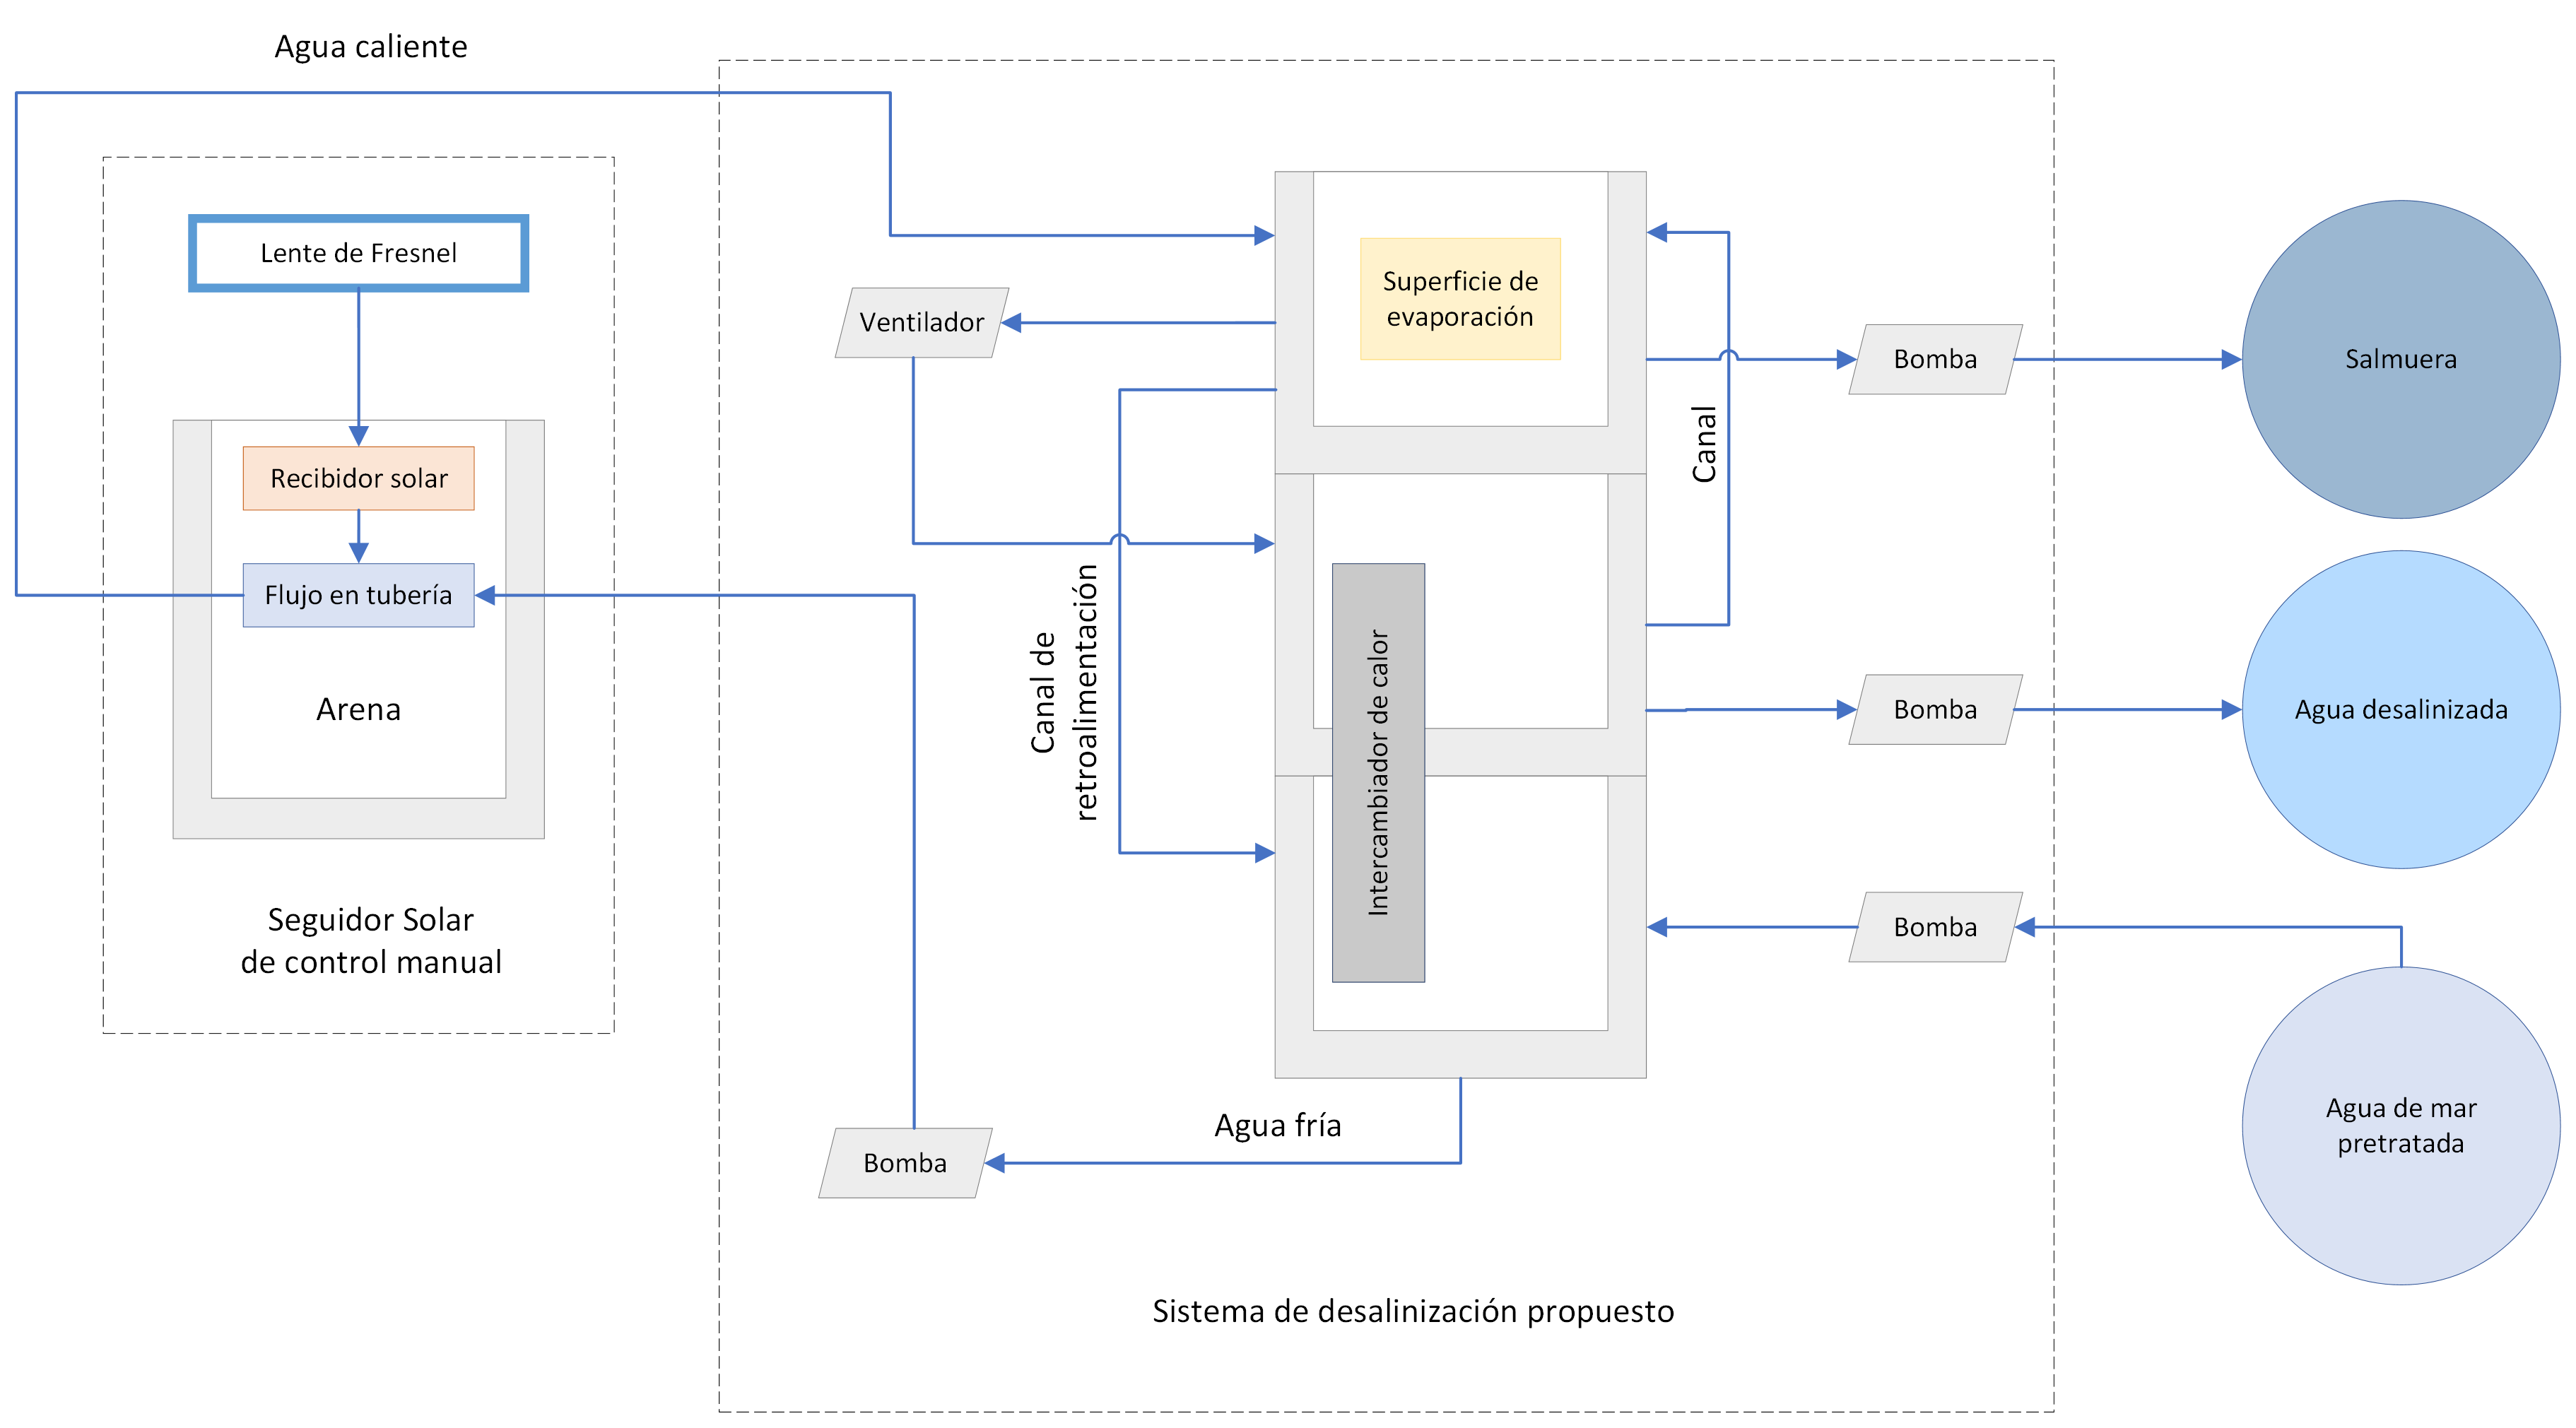
\includegraphics[
				width=\linewidth,
				height=12cm,
				keepaspectratio
			]{Resultados/Sistema/VistaGeneral.png}
			\caption{Vista general del proceso de desalinización}
			\label{fig:VistaGeneral}
		\end{figure}
		
		Gracias a este esquema se logra evitar la interferencia del vapor de agua a la superficie de calentamiento. Para validar este modelo, se usó Autodesk Inventor para la parte del diseño del sistema y Autodesk CFD para el modelado de la transferencia de calor y el flujo de aire.
		
		\subsection{Principio de funcionamiento}
			
			El desalinizador se diseñó buscando aprovechar en la medida de lo posible el calor generado por el concentrador solar, a su vez, se buscó promover la evaporación evitando volumenes grandes de agua.
			
			El desalinizador inicia su operación con un volumen de agua salada a temperatura ambiente, mediante una bomba con la capacidad de regular su caudal, una vez se alcanzan ciertas condiciones, se bombea agua hacia una tubería que se calienta mediante el recibidor solar. Una vez caliente el agua se dirige hacia una cámara donde se evapora el agua. Para favorecer este fenómeno se mantiene un volumen de agua bajo mientras que un ventilador redirige el vapor generado a una segunda cámara. El flujo de aire creado por el ventilador permite desalojar el aire saturado y renovarlo con aire más seco.
			
			El agua caliente excedente se vuelve a inyectar al inicio del ciclo mientras que el vapor generado es condensado mediante un intercambiador de calor que a su vez transmite ese calor al agua entrante.
		
	
		\subsection{Componentes y módulos del desalinizador}
			
			Tras varias propuestas se llegó a un diseño modular vertical. En la~\cref{fig:WaterModule} se puede observar el primer módulo llamado ``Módulo de reaprovechamiento térmico y bombeo'' el cual se diseñó para aprovechar el calor del vapor generado tras pasar por el ``Módulo de concentración solar'' (\cref{fig:SolarModule}) el cual se integra a un seguidor solar para calentar el agua indirectamente por medio de la lente de Fresnel.
		
		
			\begin{figure}[H]
				\centering
				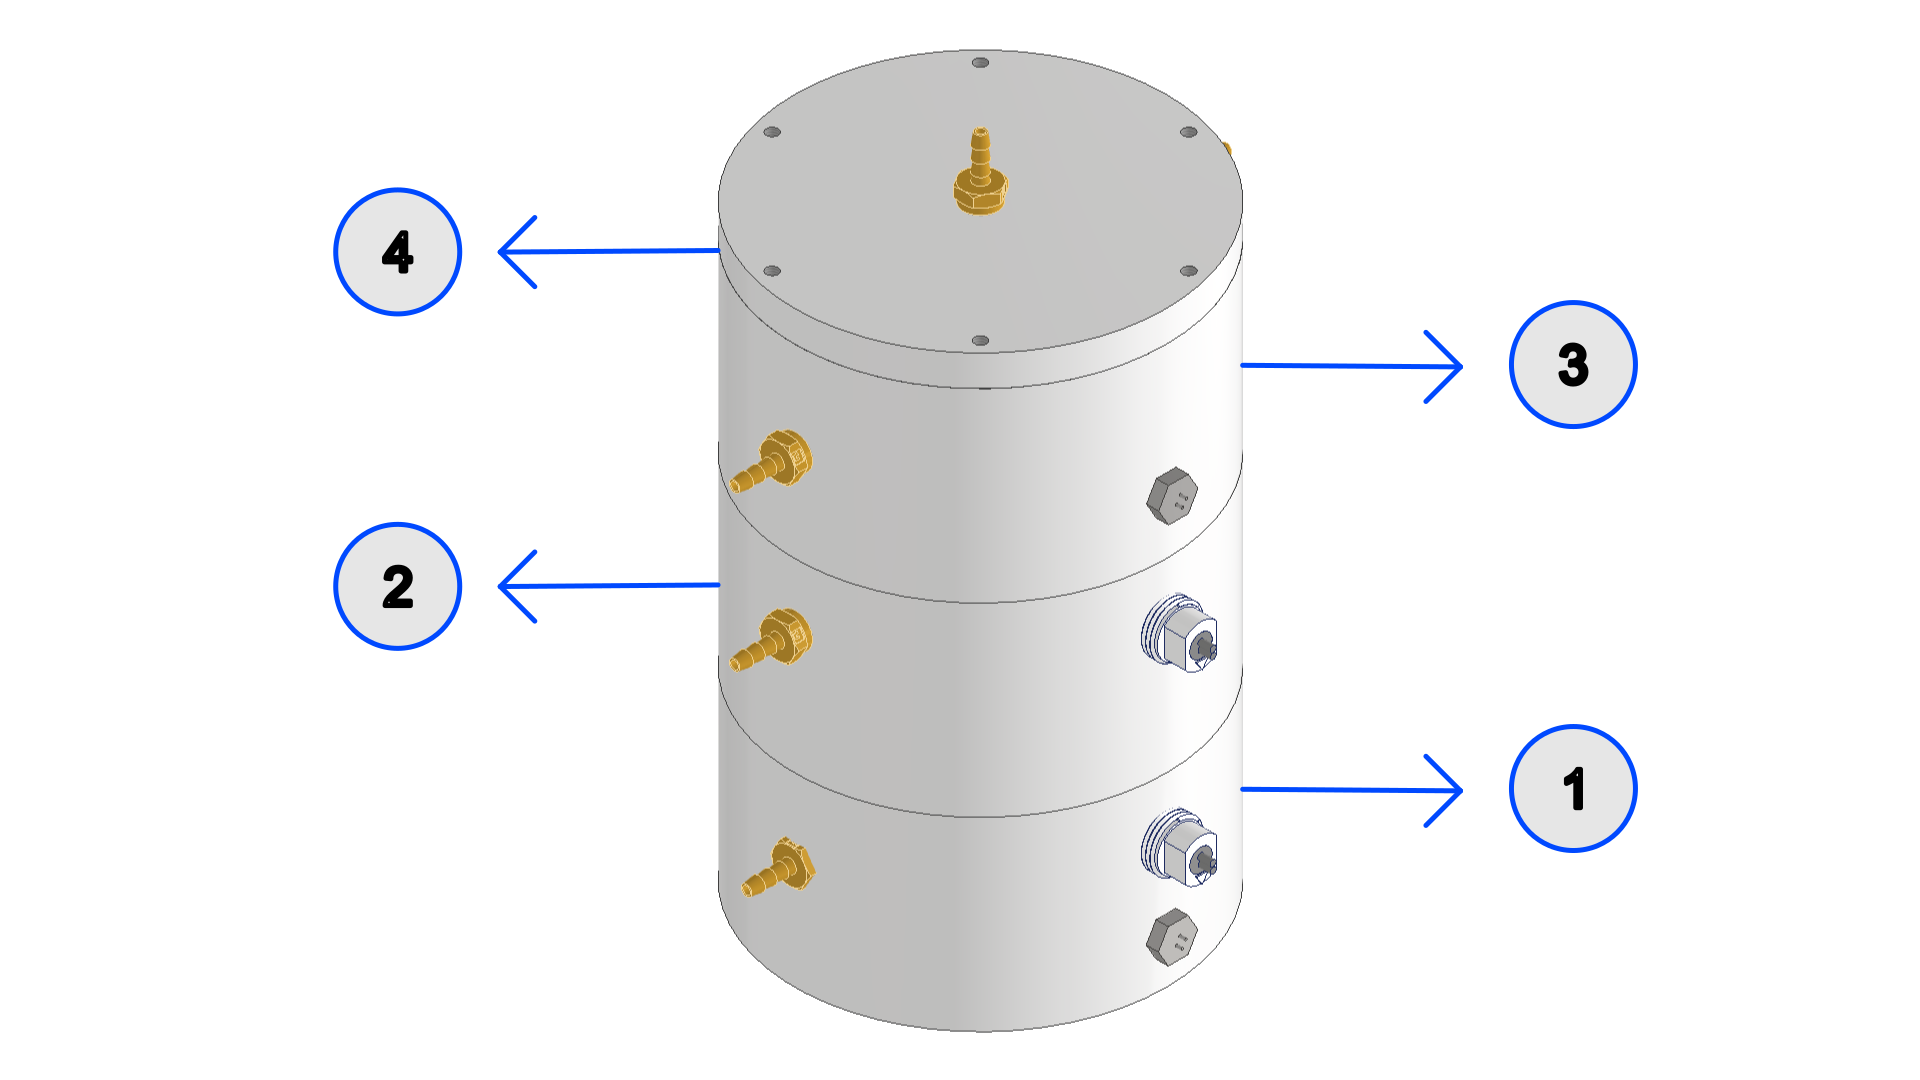
\includegraphics[
					width=\linewidth,
					height=70mm,
					keepaspectratio
				]{Resultados/Sistema/WaterModule.png}
				\caption{Propuesta del sistema desalinizador. Módulo de reaprovechamiento térmico y bombeo.}
				\label{fig:WaterModule}
			\end{figure}
			
			\begin{enumerate}[columns=2]
				\item Contenedor de agua de mar
				\item Contenedor de agua destilada
				\item Cámara de evaporación
				\item Tapa
			\end{enumerate}
			
			\begin{figure}[H]
				\centering
				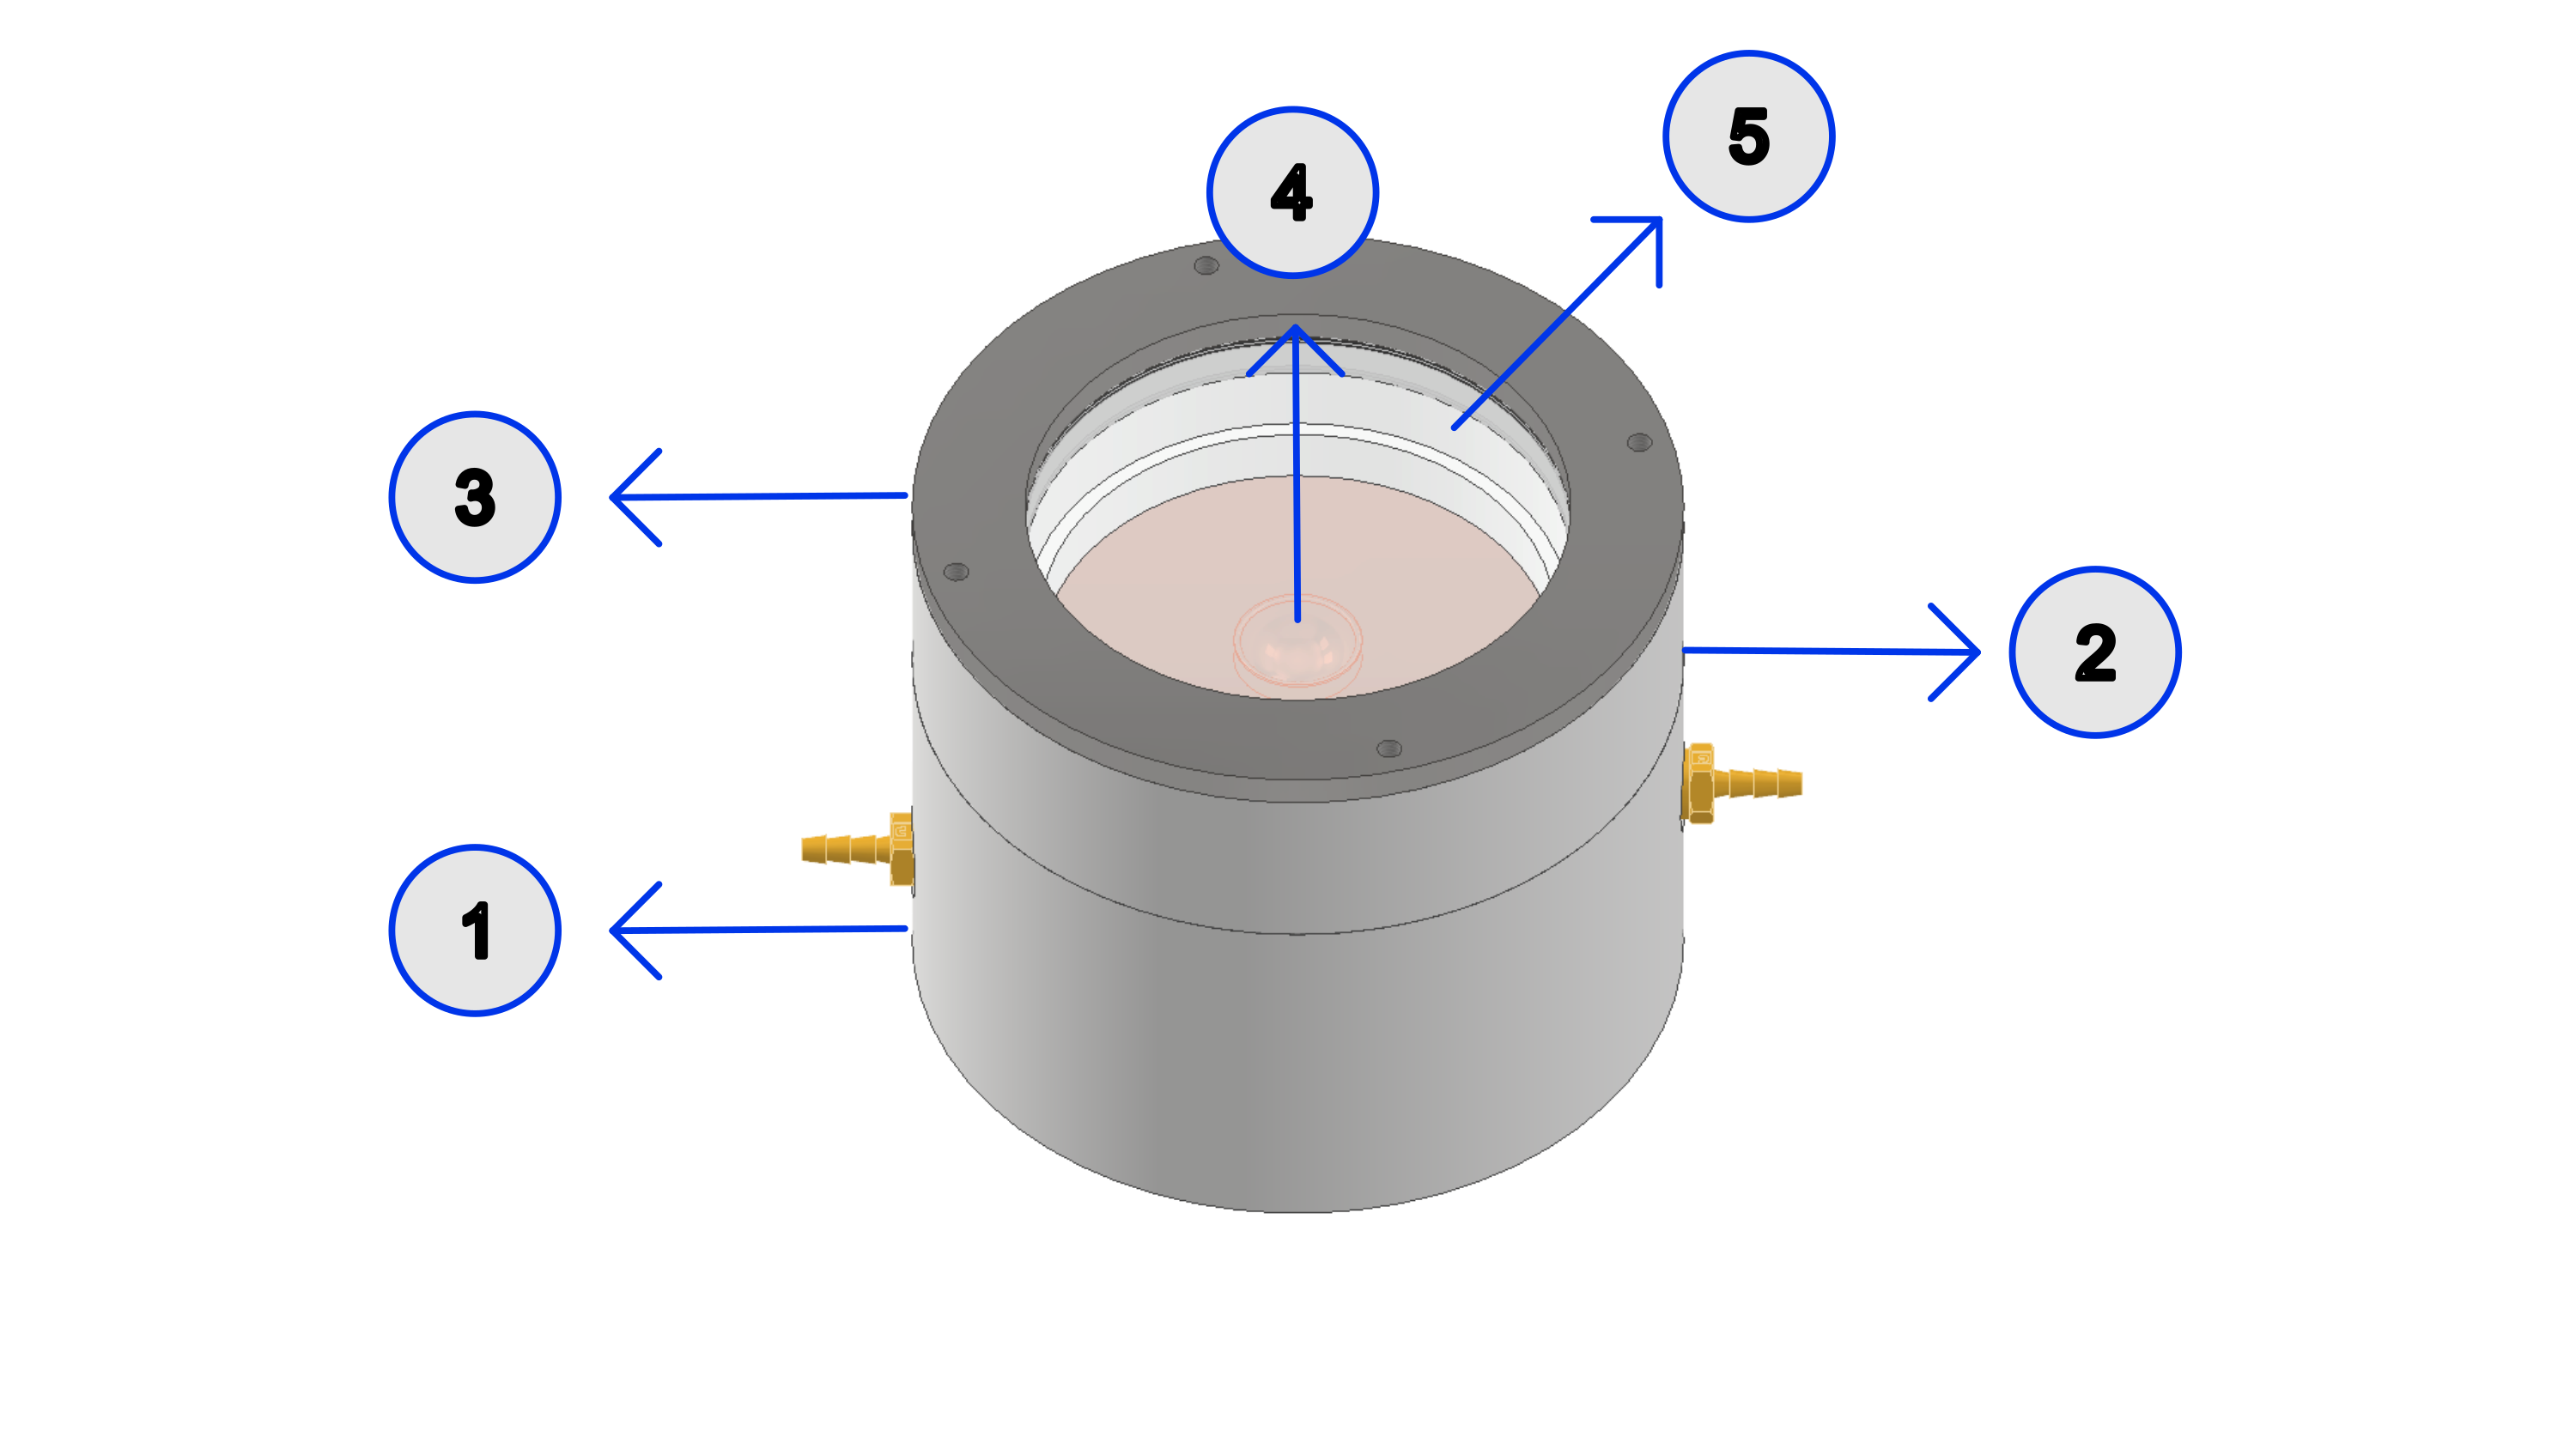
\includegraphics[
					width=\linewidth,
					height=70mm,
					keepaspectratio
				]{Resultados/Sistema/SolarModule.png}
				\caption{Propuesta del sistema desalinizador. Módulo de concentración solar.}
				\label{fig:SolarModule}
			\end{figure}
			
			\begin{enumerate}[columns=2]
				\item Cámara de transferencia de calor
				\item Soporte de lente
				\item Tapa
				\item Recibidor solar
				\item Cristal de borosilicato
			\end{enumerate}
			
			En los siguientes apartados se detallan los elementos que componen a este sistema y las funciones que desempeñan.
	
			\subsubsection{Contenedor de agua de mar}
				
				Su función básica es contener el agua a desalinizar y servir al mismo tiempo como fuente de frío para la condensación del vapor.
				
				El contenedor de agua de mar consta de 2 entradas y 1 salida.
				\begin{itemize}[columns=2]
					\item Entrada de agua de mar
					\item Entrada del excedente de agua caliente
					\item Salida hacia el calentador solar
				\end{itemize}
				
				\begin{center}
					En este módulo se monitorea la temperatura y el nivel del agua.
				\end{center}			
			
			\subsubsection{Contenedor de agua destilada}
				
				Su función básica es promover la condensación del vapor y favorecer el aumento de la temperatura del agua de entrada usando un intercambiador de calor entre la misma cámara y el contenedor de agua de mar.
				
				Este submódulo consta de 1 entrada y 2 salidas.
				
				\begin{itemize}[columns=2]
					\item Entrada de vapor caliente \columnbreak
					\item Salida para regular la presión entre cámaras
					\item Salida de agua destilada
				\end{itemize}
				
				\begin{center}
					En este módulo se monitorea el nivel del agua.
				\end{center}
							
			\subsubsection{Cámara de evaporación}
				
				Su función básica es favorecer el proceso de evaporación aumentando el área superficial por unidad de volumen. Para incrementar la evaporación efectiva se acopló un ventilador que permite desalojar el aire saturado además de promover el flujo del aire.
				
				En una segunda revisión se formuló la posibilidad de agregar elementos que permitieran aumentar el área de contacto del agua con el aire debido a que en realidad se trata de un espacio reducido, por lo que se propone el diseño visto en la~\cref{fig:EvaporationSurface}
				
				\begin{figure}[H]
					\centering
					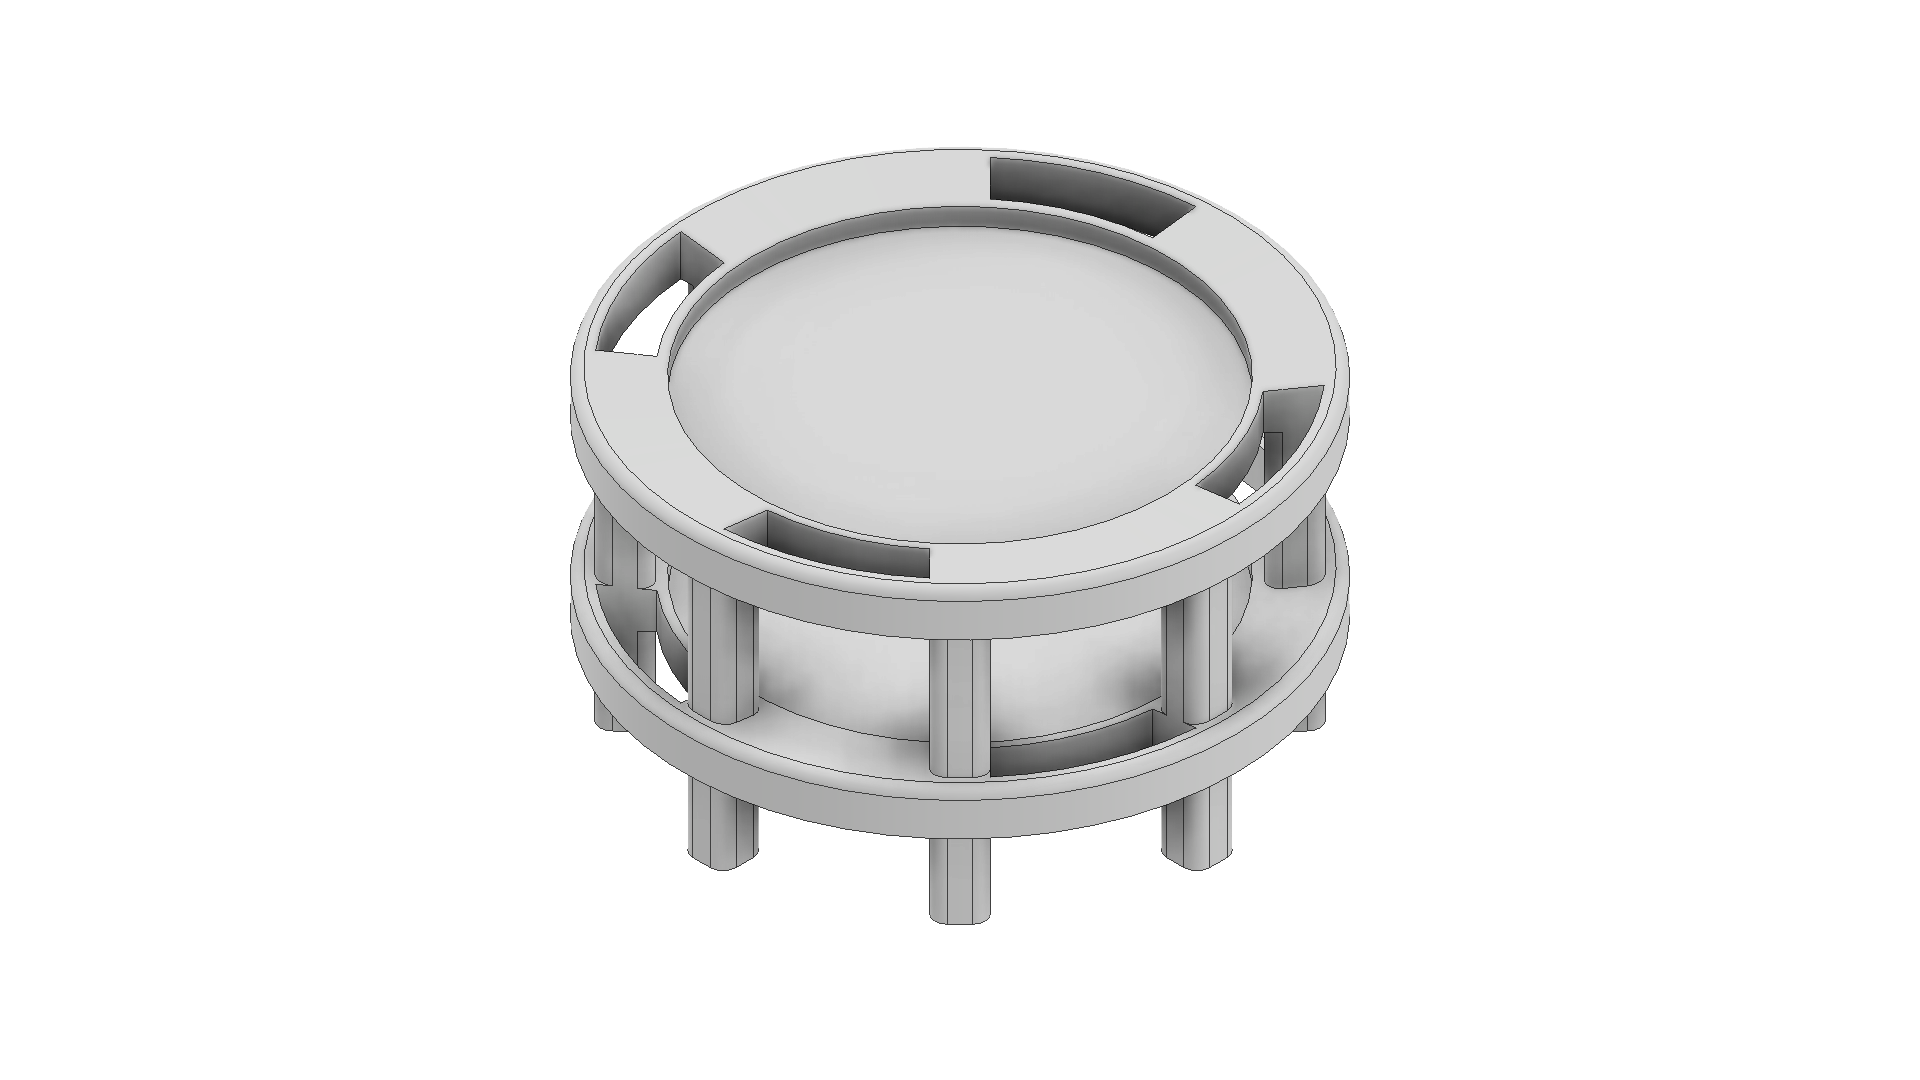
\includegraphics[
						width=\linewidth,
						height=70mm,
						keepaspectratio
					]{Resultados/Sistema/EvaporationSurface.png}
					\caption{Diseño sugerido para aumentar el área de evaporación dentro de la cámara}
					\label{fig:EvaporationSurface}
				\end{figure}
				
				Este submódulo consta de 2 entradas y 2 salidas.
				
				\begin{itemize}[columns=2]
					\item Entrada de agua caliente
					\item Entrada de aire de recirculación
					\item Salida de vapor caliente
					\item Salida de salmuera
				\end{itemize}
				
				\begin{center}
					En este módulo se monitorea la temperatura del agua.
				\end{center}
			
			\subsubsection{Módulo de concentración solar}
				
				Este módulo se divide en dos partes por cuestiones de ensamble y manufactura. La parte superior se encarga de soportar un cristal de borosilicato por el cual atraviesan los rayos solares. Este cristal nos permite mantener un mejor aislamiento térmico del recibidor solar así como evitar la exposición directa al ambiente.
				
				Por otra parte, en el submódulo inferior ocurre el intercambio de calor entre el recibidor solar y el agua. Esto se logra por medio de la conducción de calor entre el recibidor y una tubería de cobre. La elección de la tubería de cobre se dio debido a su alta conductividad térmica, flexibilidad, disponibilidad y costos, ya que en un inicio se planteó el uso de acero galvanizado y de acero inoxidable 316, sin embargo, como se mostrará en las simulaciones siguientes no resultaba buen conductor térmico además de ser difícilmente manufacturable; también se descartó el uso de tuberías de aluminio 5052 debido a su escaza disponibilidad.
				
				Este submódulo consta de 1 entrada y 1 salida.
				
				\begin{itemize}[columns=2]
					\item Entrada de agua fría
					\item Salida de agua caliente
				\end{itemize}
				
				\begin{center}
					En este módulo se monitorea la temperatura del recibidor solar.
				\end{center}
		
		\subsection{Simulaciones del sistema desalinizador}
			
			Se realizaron varias simulaciones de transferencia de calor con el fin de validar los diseños propuestos, los materiales seleccionados y el caudal propuesto durante el desarrollo experimental. A su vez, se realizaron simulaciones del flujo de aire en la cámara de evaporación con el fin de validar el diseño visto en la~\cref{fig:EvaporationSurface}.
			
			\subsubsection{Materiales y geometría}
			
				\textbf{Transferencia de calor}\par
			
				Con el fin de observar el desempeño de los materiales a utilizar para intercambiar calor con el recibidor solar, se simuló transferencia de calor con cobre, aluminio y acero inoxidable bajo condiciones favorables (Alta generación de calor). De estas simulaciones se concluyó que:
				
				\begin{enumerate}
					\item El acero inoxidable no proporciona una conducción suficiente de calor, ya que el recibidor empieza a sobrecalentarse mientras que el agua no adquiere la temperatura suficiente. Si se observa detenidamente la~\cref{fig:stainless-steel-heat-transfer} se observa que el agua se calienta cuando está más cerca del recibidor, sin embargo, el calor no llega a toda la tubería, por lo que esta se vuelve a enfriar una vez que se aleja del recibidor. Además, el recibidor comienza a sobrecalentarse al no deshacerse del calor, transfiriéndolo a los aislantes térmicos y los alrededores del recibidor. 
					\item El cobre es un buen candidato, ya que la tubería se calienta uniforme y rápidamente, además, el agua adquiere una temperatura poco menor que la del recibidor.
					
					\item El aluminio 5052 es un buen candidato, ya que la tubería se calienta rápidamente, sin embargo, incrementa la diferencia entre la temperatura del agua y la del recibidor en contraste con el cobre, sin mencionar que el agua se calienta de manera menos uniforme.
				\end{enumerate}
				
				\begin{figure}[H]
					\centering
					\begin{subfigure}[t]{\linewidth}
						\centering
						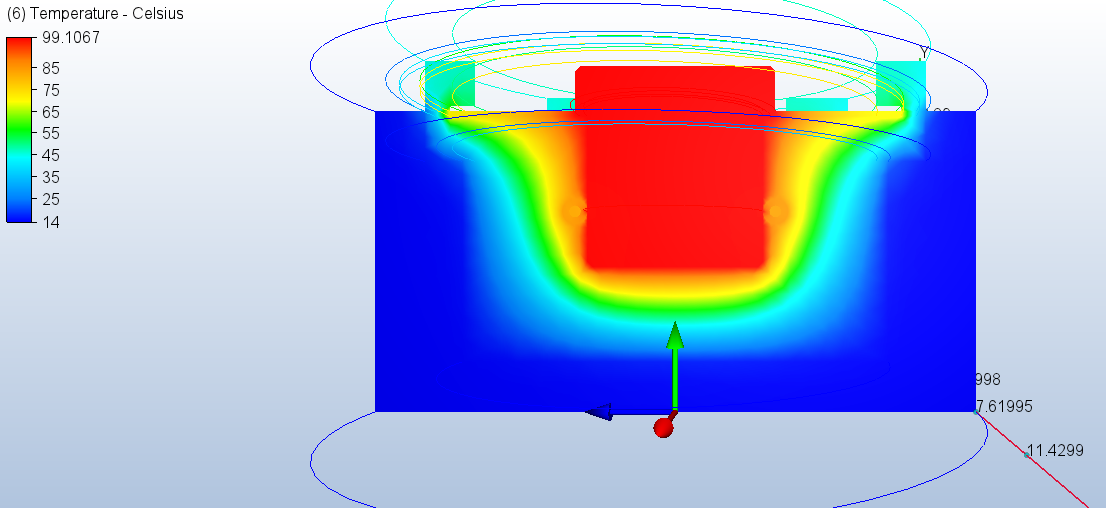
\includegraphics[
							width=\linewidth,
							height = 60mm,
							keepaspectratio
						]{Resultados/Simulaciones/50W-StainleesSteel-15C-9mlpm-middle.png}
						\caption{Corte en el centro del recibidor solar y su transferencia de calor hacia el acero inoxidable 316}
						\label{fig:50W-StainleesSteel-15C-9mlpm-middle}
					\end{subfigure}
				\end{figure}

				\begin{figure}[H]\ContinuedFloat
					\begin{subfigure}[t]{\linewidth}
						\centering
						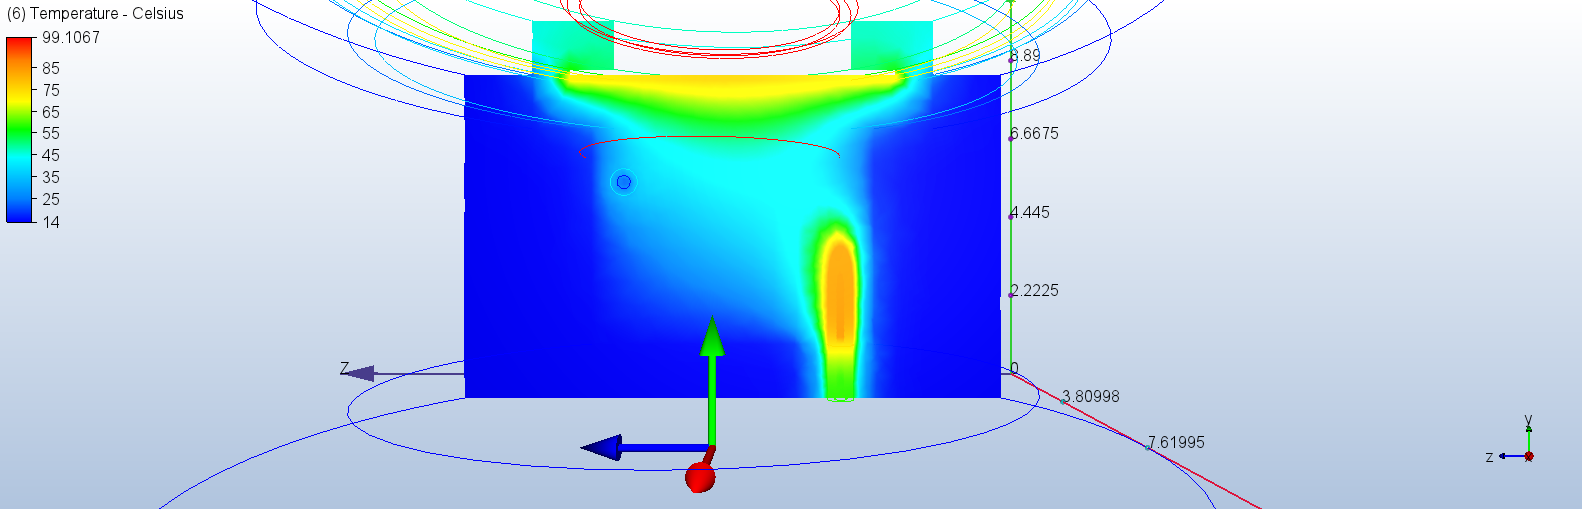
\includegraphics[
							width=\linewidth,
							height = 60mm,
							keepaspectratio
						]{Resultados/Simulaciones/50W-StainleesSteel-15C-9mlpm.png}
						\caption{Corte en la entrada y salida del agua de mar}
						\label{fig:50W-StainleesSteel-15C-9mlpm}
					\end{subfigure}
					\hfill
					\caption{Transferencia de calor en el acero inoxidable}
					\label{fig:stainless-steel-heat-transfer}
				\end{figure}
				
				\begin{figure}[H]
					\centering
					\begin{subfigure}[t]{\linewidth}
						\centering
						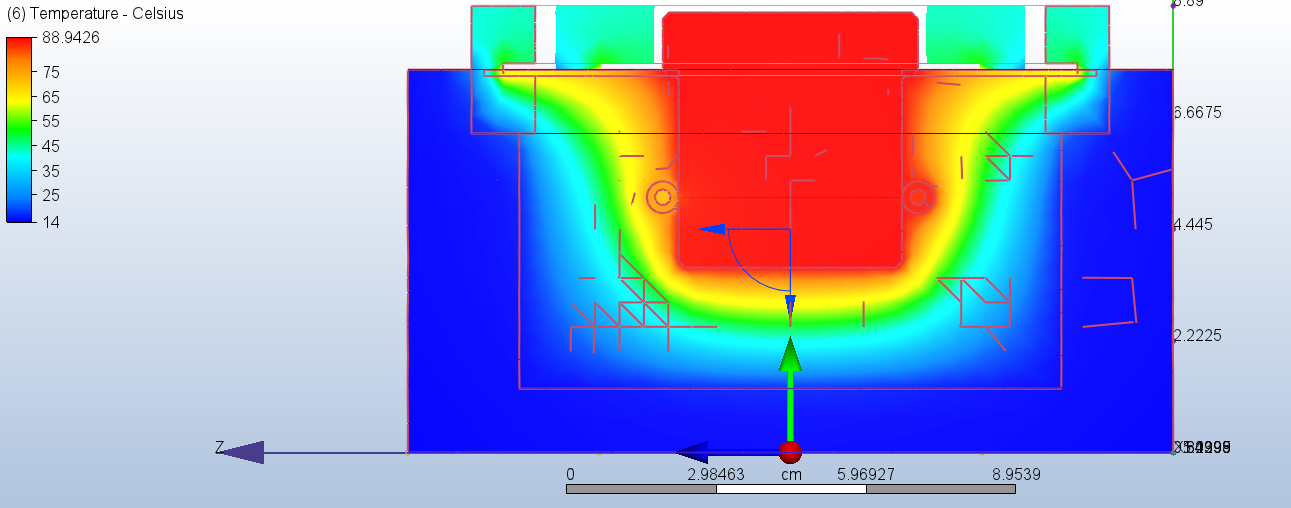
\includegraphics[
							width=\linewidth,
							height = 60mm,
							keepaspectratio
						]{Resultados/Simulaciones/50WCopper15C9mlpm-middle.png}
						\caption{Corte en el centro del recibidor solar y su transferencia de calor hacia el cobre}
						\label{fig:50WCopper15C9mlpm-middle}
					\end{subfigure}
				\end{figure}

				\begin{figure}[H]\ContinuedFloat
					\begin{subfigure}[t]{\linewidth}
						\centering
						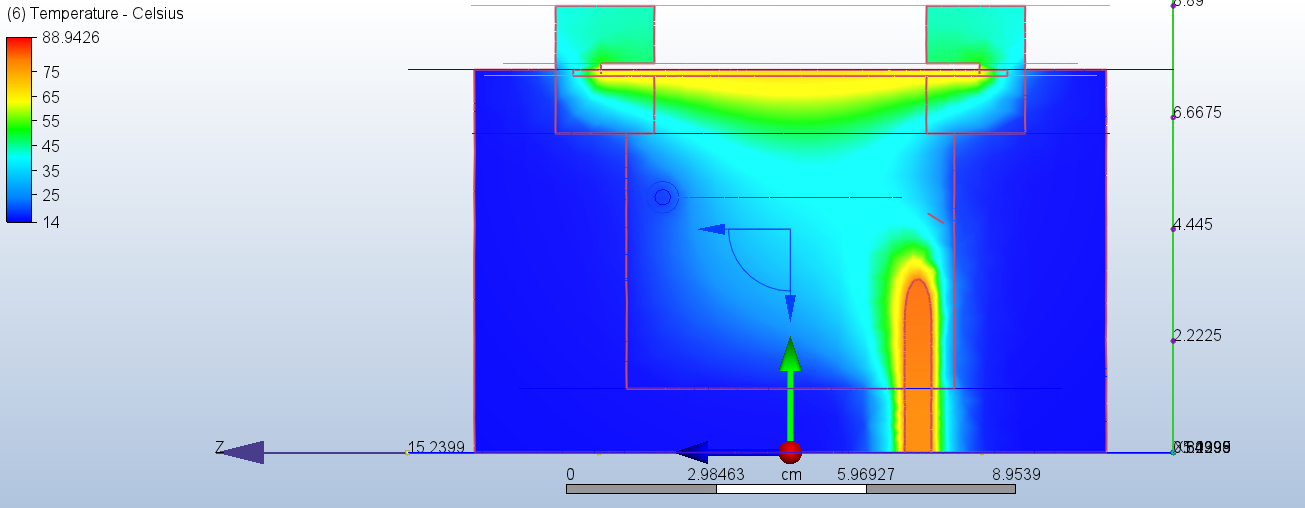
\includegraphics[
							width=\linewidth,
							height = 60mm,
							keepaspectratio
						]{Resultados/Simulaciones/50WCopper15C9mlpm.png}
						\caption{Corte en la entrada y salida del agua de mar}
						\label{fig:50WCopper15C9mlpm}
					\end{subfigure}
					\hfill
					\caption{Transferencia de calor en el cobre}
					\label{fig:copper-heat-transfer}
				\end{figure}
				
				\begin{figure}[H]
					\centering
					\begin{subfigure}[t]{\linewidth}
						\centering
						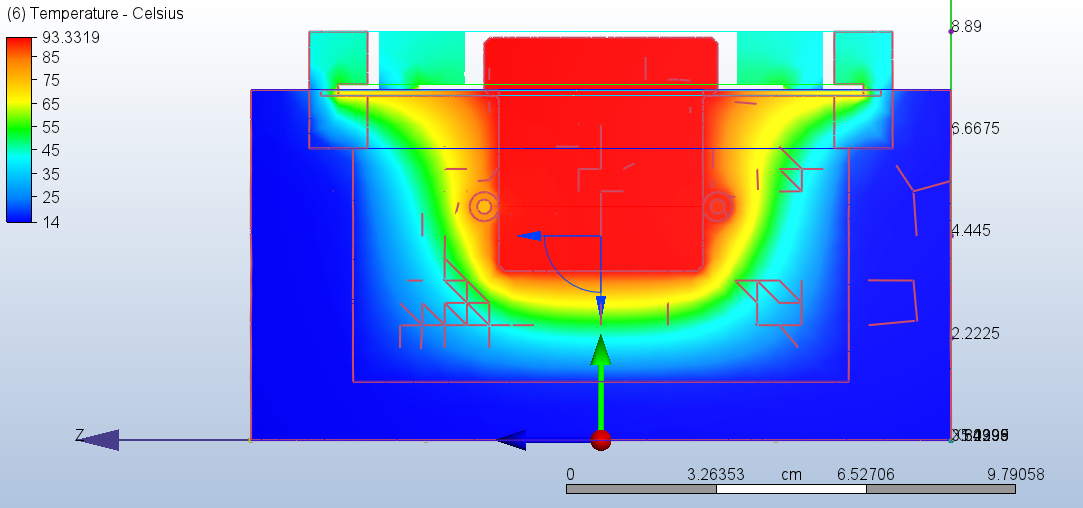
\includegraphics[
							width=\linewidth,
							height = 60mm,
							keepaspectratio
						]{Resultados/Simulaciones/50WAluminum15C9mlpm-middle.png}
						\caption{Corte en el centro del recibidor solar y su transferencia de calor hacia el aluminio}
						\label{fig:50WAluminum15C9mlpm-middle}
					\end{subfigure}
				\end{figure}

				\begin{figure}[H]\ContinuedFloat
					\begin{subfigure}[t]{\linewidth}
						\centering
						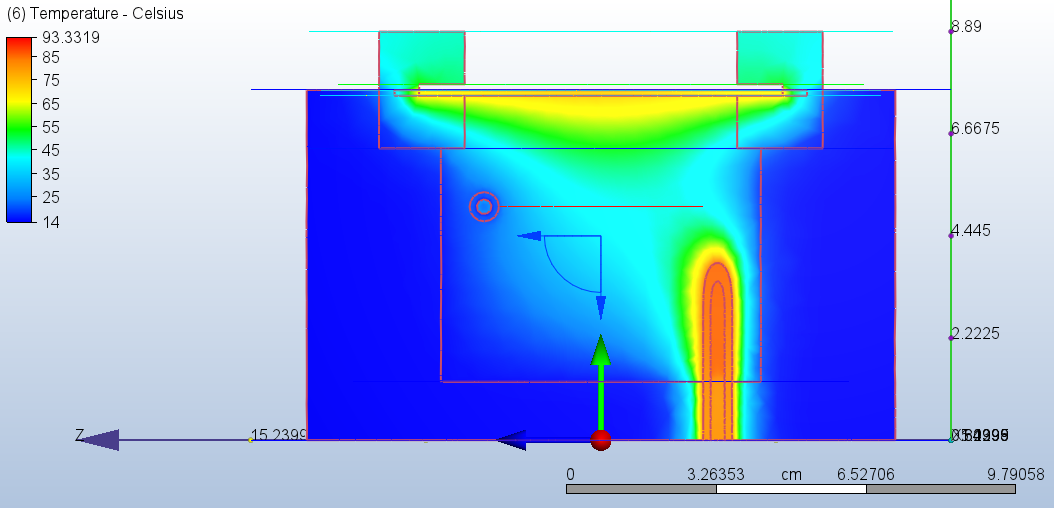
\includegraphics[
							width=\linewidth,
							height = 60mm,
							keepaspectratio
						]{Resultados/Simulaciones/50WAluminum15C9mlpm.png}
						\caption{Corte en la entrada y salida del agua de mar}
						\label{fig:50WAluminum15C9mlpm}
					\end{subfigure}
					\hfill
					\caption{Transferencia de calor en el aluminio}
					\label{fig:aluminum-heat-transfer}
				\end{figure}
				
				Se simularon 300 segundos de transferencia de calor de los tres materiales bajo las condiciones halladas en el desarrollo experimental en lugar de buscar la convergencia, ya que esto requeriría un tiempo mucho mayor y observando el comportamiento de la temperatura del recibidor se concluyó que la información proporcionada fue suficiente para llegar a una conjetura.
				
				De las simulaciones se observó que la temperatura del recibidor solar crecía más rápidamente que la temperatura del agua de salida; en cambio, el cobre y el aluminio tuvieron mejores respuestas.
				
				\textit{Producto de estas simulaciones}
				
				Las anteriores simulaciones ayudaron a comprender un poco más la respuesta del sistema y con base en ello se tomaron las siguientes decisiones.
				
				\begin{itemize}
					\item Se descartó el uso de acero inoxidable como material para la tubería
					\item Se aceptó el uso de aluminio 5052 como material para la tubería pero se identificaron ciertas limitaciones en contraste con el cobre como menor ductibilidad, menor transferencia de calor pero mayor resistencia a la corrosión.
					\item Los criterios de manufacturabilidad cambiaron cuando se eligió el cobre como material para la tubería. Como resultado, se propuso un nuevo diseño para mejorar la homogeneidad de la temperatura del agua, esto se muestra en la~\cref{fig:FuzzyUniverse}.
				\end{itemize}
				
				
				\textbf{Flujo de aire en la cámara de evaporación}\par
			
				La superficie de evaporación vista en la~\cref{fig:EvaporationSurface} incrementa a más del doble la superficie de evaporación y no disminuye sustancialmente el flujo de aire dentro de la cámara como se observa en la~\cref{fig:AirflowInEvaporationChamber}, por lo cual se justifica parcialmente su incorporación al desalinizador dado que falta evaluar su influencia en la acumulación de sales dentro de la cámara.
				
				\begin{figure}[H]
					\centering
					\begin{subfigure}[t]{0.45\linewidth}
						\centering
						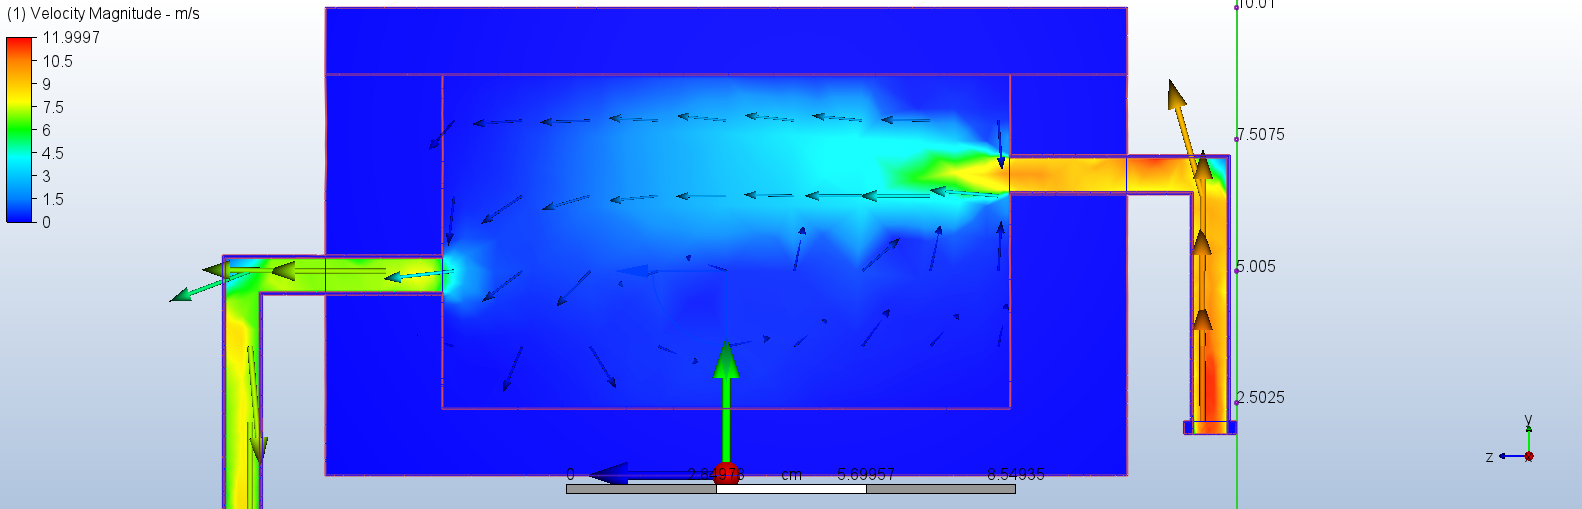
\includegraphics[
							width=\linewidth,
							height = 60mm,
							keepaspectratio
						]{Resultados/Simulaciones/AirflowWithoutEvaporationSurface.png}
						\caption{Flujo de aire sin superficie de evaporación}
						\label{fig:AirflowWithoutEvaporationSurface}
					\end{subfigure}
					\hfill
					\begin{subfigure}[t]{0.45\linewidth}
						\centering
						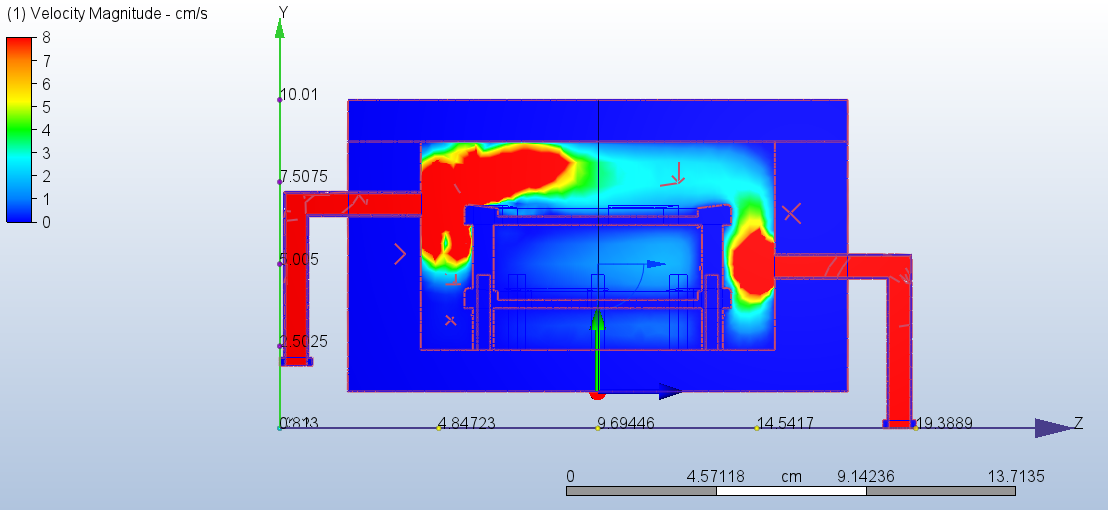
\includegraphics[
							width=\linewidth,
							height = 60mm,
							keepaspectratio
						]{Resultados/Simulaciones/AirflowWithEvaporationSurface.png}
						\caption{Flujo de aire con superficie de evaporación}
						\label{fig:AirflowWithEvaporationSurface}
					\end{subfigure}
					\caption{Flujo de aire en la cámara de evaporación}
					\label{fig:AirflowInEvaporationChamber}
				\end{figure}
		
			
				
				
	\section{Control del sistema}
	
		Tras el estudio y comparación de las ventajas y desventajas de diferentes métodos de control numérico se concluyó que el método de control difuso se acoplaba mejor a las necesidades del sistema ya que:
		
		\begin{itemize}
			\item El modelo de contro difuso permite hacer razonamientos para evaluar el grado de certidumbre de una afirmación en vez de limitarse a una lógica binaria donde se producen saltos de una afirmación a otra.
			\item Permite crear un modelo de control basado en reglas fácilmente interpretables
			\item No requiere un modelo matemático u aproximación numérica del proceso, sino, en conocimiento empírico, lo cual es muy beneficioso, ya que tanto el proceso de evaporación como el de ebullición es un fenómeno muy complejo y difícilmente modelable.
			\item Permite tomar decisiones de conocimientos y datos inexactos de forma similar al razonamiento humano
		\end{itemize}
		
		El control difuso se centró en la regulación del flujo de agua de mar debido a la naturaleza variable e intermitente de la fuente de energía. En consecuencia, resultó fundamental supervisar la energía recibida y ajustar el caudal en función de esta variabilidad. Además, se implementó un segundo sistema de control independiente que controla los niveles de agua en el módulo de reaprovechamiento térmico y bombeo.
		
		\subsection{Sensores y componentes, calibración y caracterización}\label{subsec:calibración}
		
			En esta sección se detalla el proceso de ajuste y caracterización de los sensores y la bomba que regula el flujo de agua, estas calibraciones resultan indispensables para el correcto funcionamiento del método de control.
			
			\textbf{Termistores}\par
			
			Para caracterizar los termistores se refirió a un set de datos que reflejan la respuesta óhmica al aplicarse cierta temperatura; el código visto en~\cref{ch:steinhart-code} nos permite hallar los coeficientes de Steinhart-Hart para este modelo.
			
			Se halló que:
			
			\begin{itemize}[columns=3]
				\item A = \num{1.12866e-3}
				\item B = \num{2.3422e-4}
				\item C = \num{8.7159e-8}
			\end{itemize}
			
			\textbf{EZO-PMP}\par
			
			La bomba peristáltica EZO-PMP permite una calibración manual, para ello se recreó la configuración vista en la~\cref{fig:Calibración-bomba}
			
			\begin{figure}[H]
				\centering
				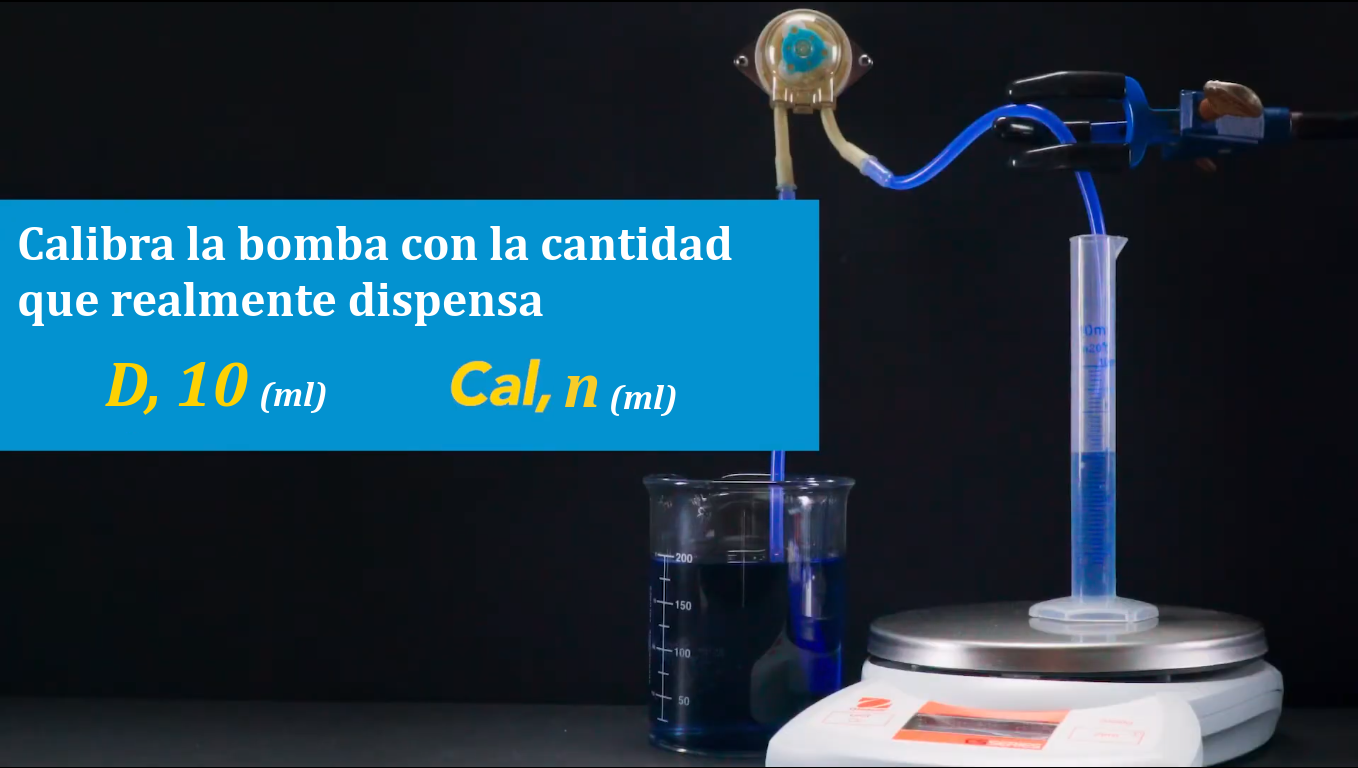
\includegraphics[
					width=\linewidth,
					height=65mm,
					keepaspectratio
				]{Resultados/Control/PumpCalibration.png}
				\caption{Arreglo para la calibración de la bomba EZO-PMP}
				\floatfoot{Imagen adaptada de \cite{atlas_scientific_llc_ezo-pmp_2020}}
				\label{fig:Calibración-bomba}
			\end{figure}
		
		\subsection{Modelo y reglas del control difuso}
				
			En esta sección se presenta evidencia de las simulaciones realizadas, las cuales sirvieron para delimitar el universo de discurso de las variables difusas y comprender su impacto en el modelo.
				
			Se decidió restringir las variables difusas exclusivamente a la temperatura del agua de entrada y la del recibidor solar. Esta decisión se tomó considerando que un gran número de variables podría aumentar exponencialmente la complejidad del algoritmo y las reglas.
			
			En la~\cref{fig:FuzzyUniverse} se muestra brevemente evidencia de las diferentes simulaciones hechas. En estas se estudiaron las respuestas al variar la temperatura del agua entrante, el caudal y el calor capturado por el concentrador solar.
								
			\begin{figure}[H]
				\centering
				\includegraphics[
					width=\linewidth,
					height = 60mm,
					keepaspectratio
				]{Resultados/Simulaciones/FuzzyUniverse.png}
				\caption{Captura de pantalla de Autodesk CFD mostrando una vista general de las simulaciones realizadas}
				\label{fig:FuzzyUniverse}
			\end{figure}
			
			Durante la corrida de las simulaciones se observó que:
			
			\begin{enumerate}
				\item En esta nueva geometría de la tubería de cobre, el agua de salida adquiere prácticamente la temperatura del agua solar una vez se estabiliza el intercambio de calor. Cabe resaltar que esta temperatura y la temperatura del agua a evaporar son distintas.
				\item La variación del flujo de agua tiene el mayor impacto en el sistema; un cambio repentino en el flujo de agua tiene un impacto significativo en la temperatura del agua de salida.
				\item La variación de la temperatura del agua entrante tiene un impacto notable en la temperatura del agua de salida, aunque es necesario un rango amplio para notar esta diferencia.
			\end{enumerate} 
						
			Se propuso entonces utilizar una función de membresía triangular para el caudal, ya que representa con mayor precisión los cambios bruscos que produce en la respuesta del sistema. En cuanto a la temperatura del receptor solar, se propuso una función gaussiana debido a que se ajusta más al comportamiento observado.
			
			Posteriormente se definieron 5 variables lingüísticas y sus respectivas membresías, esras son visibles en las~\cref{fig:var-membership-functions,fig:FlowVelocity}.
			
			\begin{figure}[H]
				\centering
				\begin{subfigure}[t]{0.45\linewidth}
					\centering
					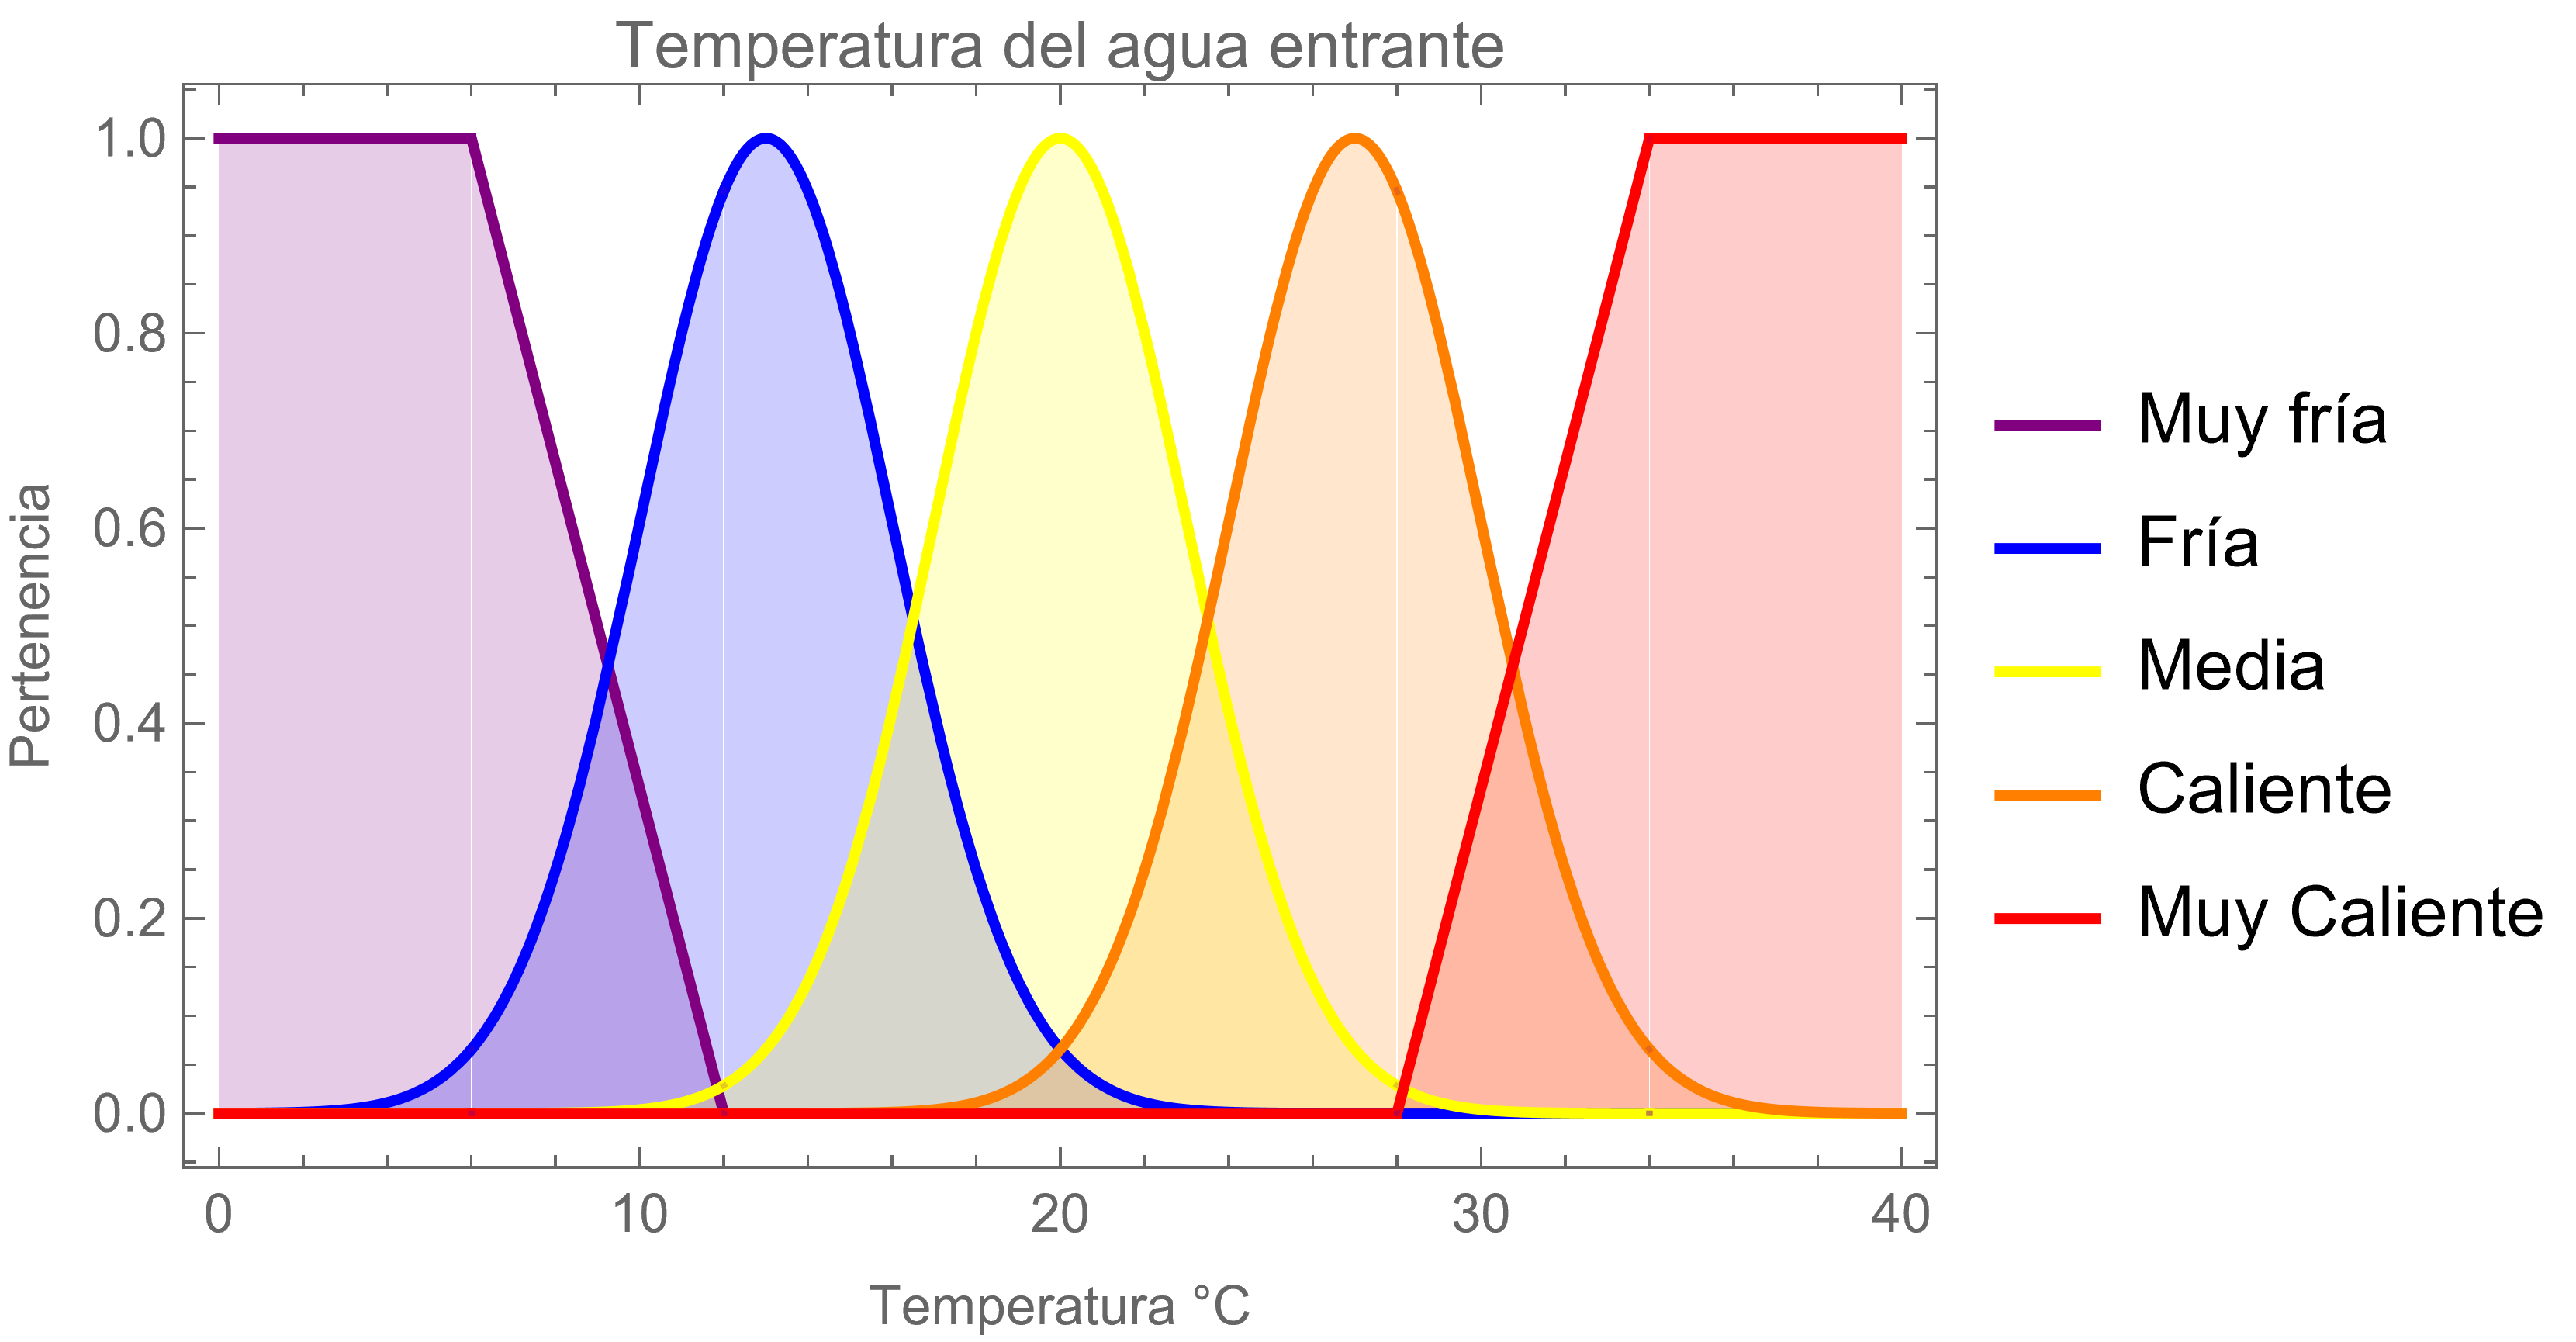
\includegraphics[
						width=\linewidth,
						height = 60mm,
						keepaspectratio
					]{Resultados/Control/SeawaterTemperature.png}
					\caption{Funciones de membresía de la temperatura del agua de mar entrante}
					\label{fig:SeawaterTemperature}
				\end{subfigure}
				\hfill
				\begin{subfigure}[t]{0.45\linewidth}
					\centering
					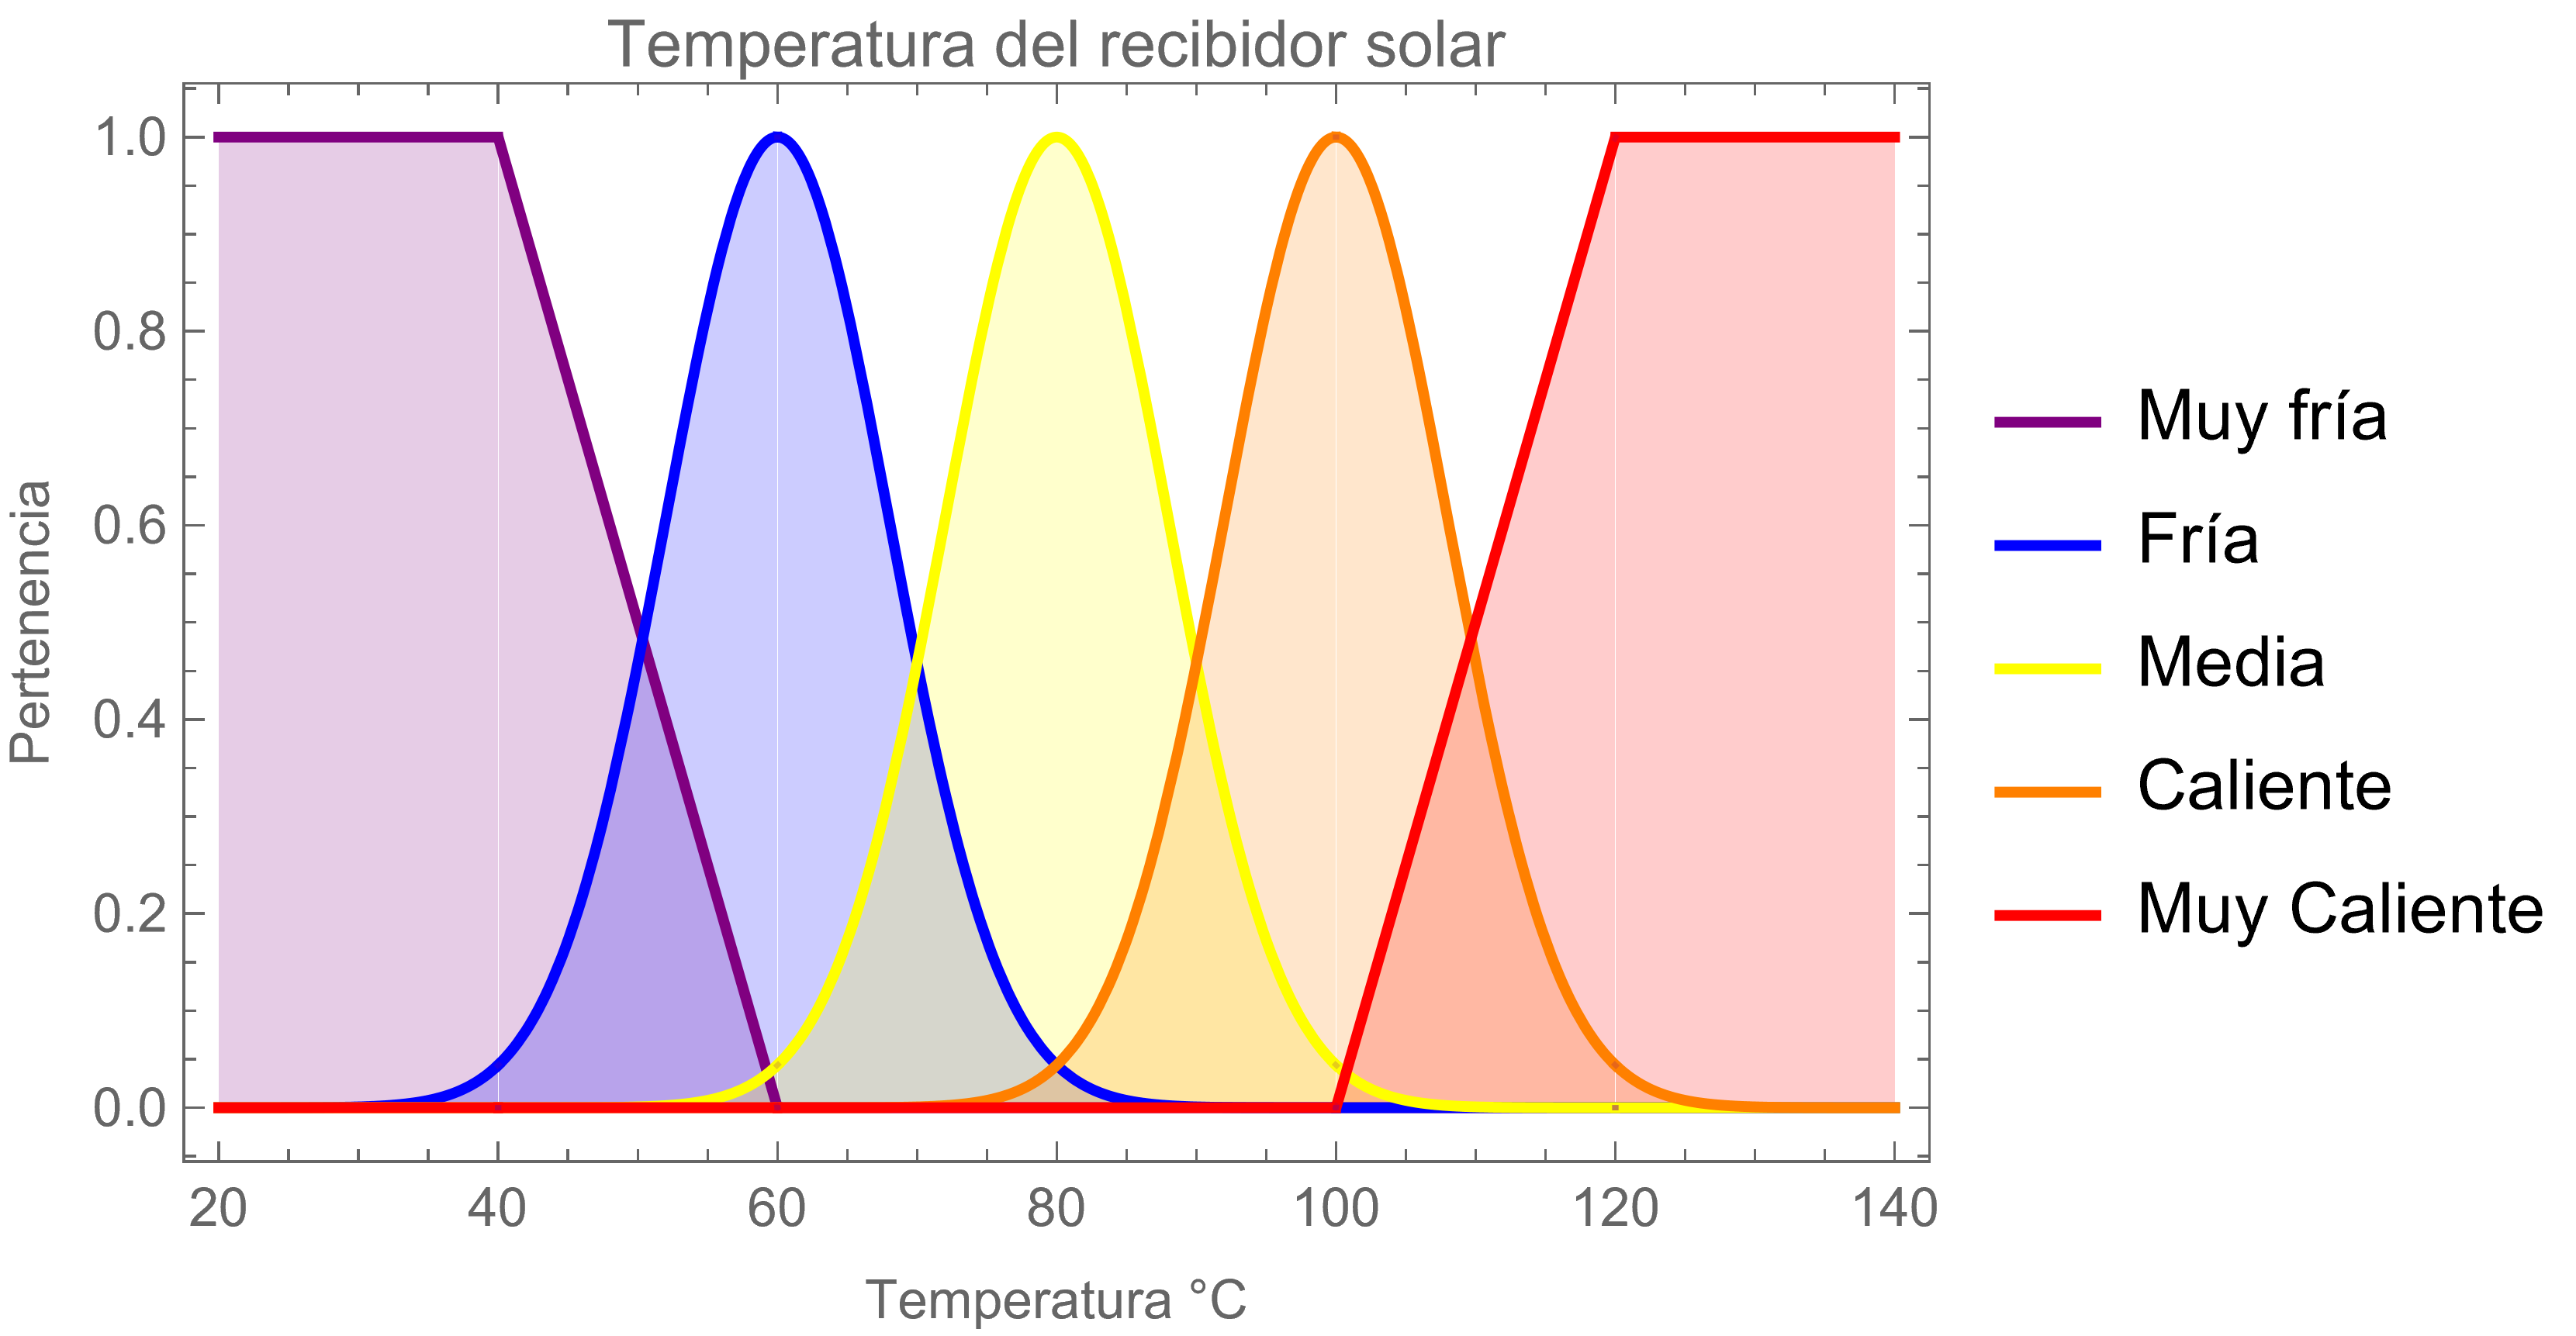
\includegraphics[
						width=\linewidth,
						height = 60mm,
						keepaspectratio
					]{Resultados/Control/SolarReceiverTemperature.png}
					\caption{Funciones de membresía de la temperatura del recibidor solar}
					\label{fig:SolarReceiverTemperature}
				\end{subfigure}
			\end{figure}
			
			\begin{figure}[H]
				\centering
				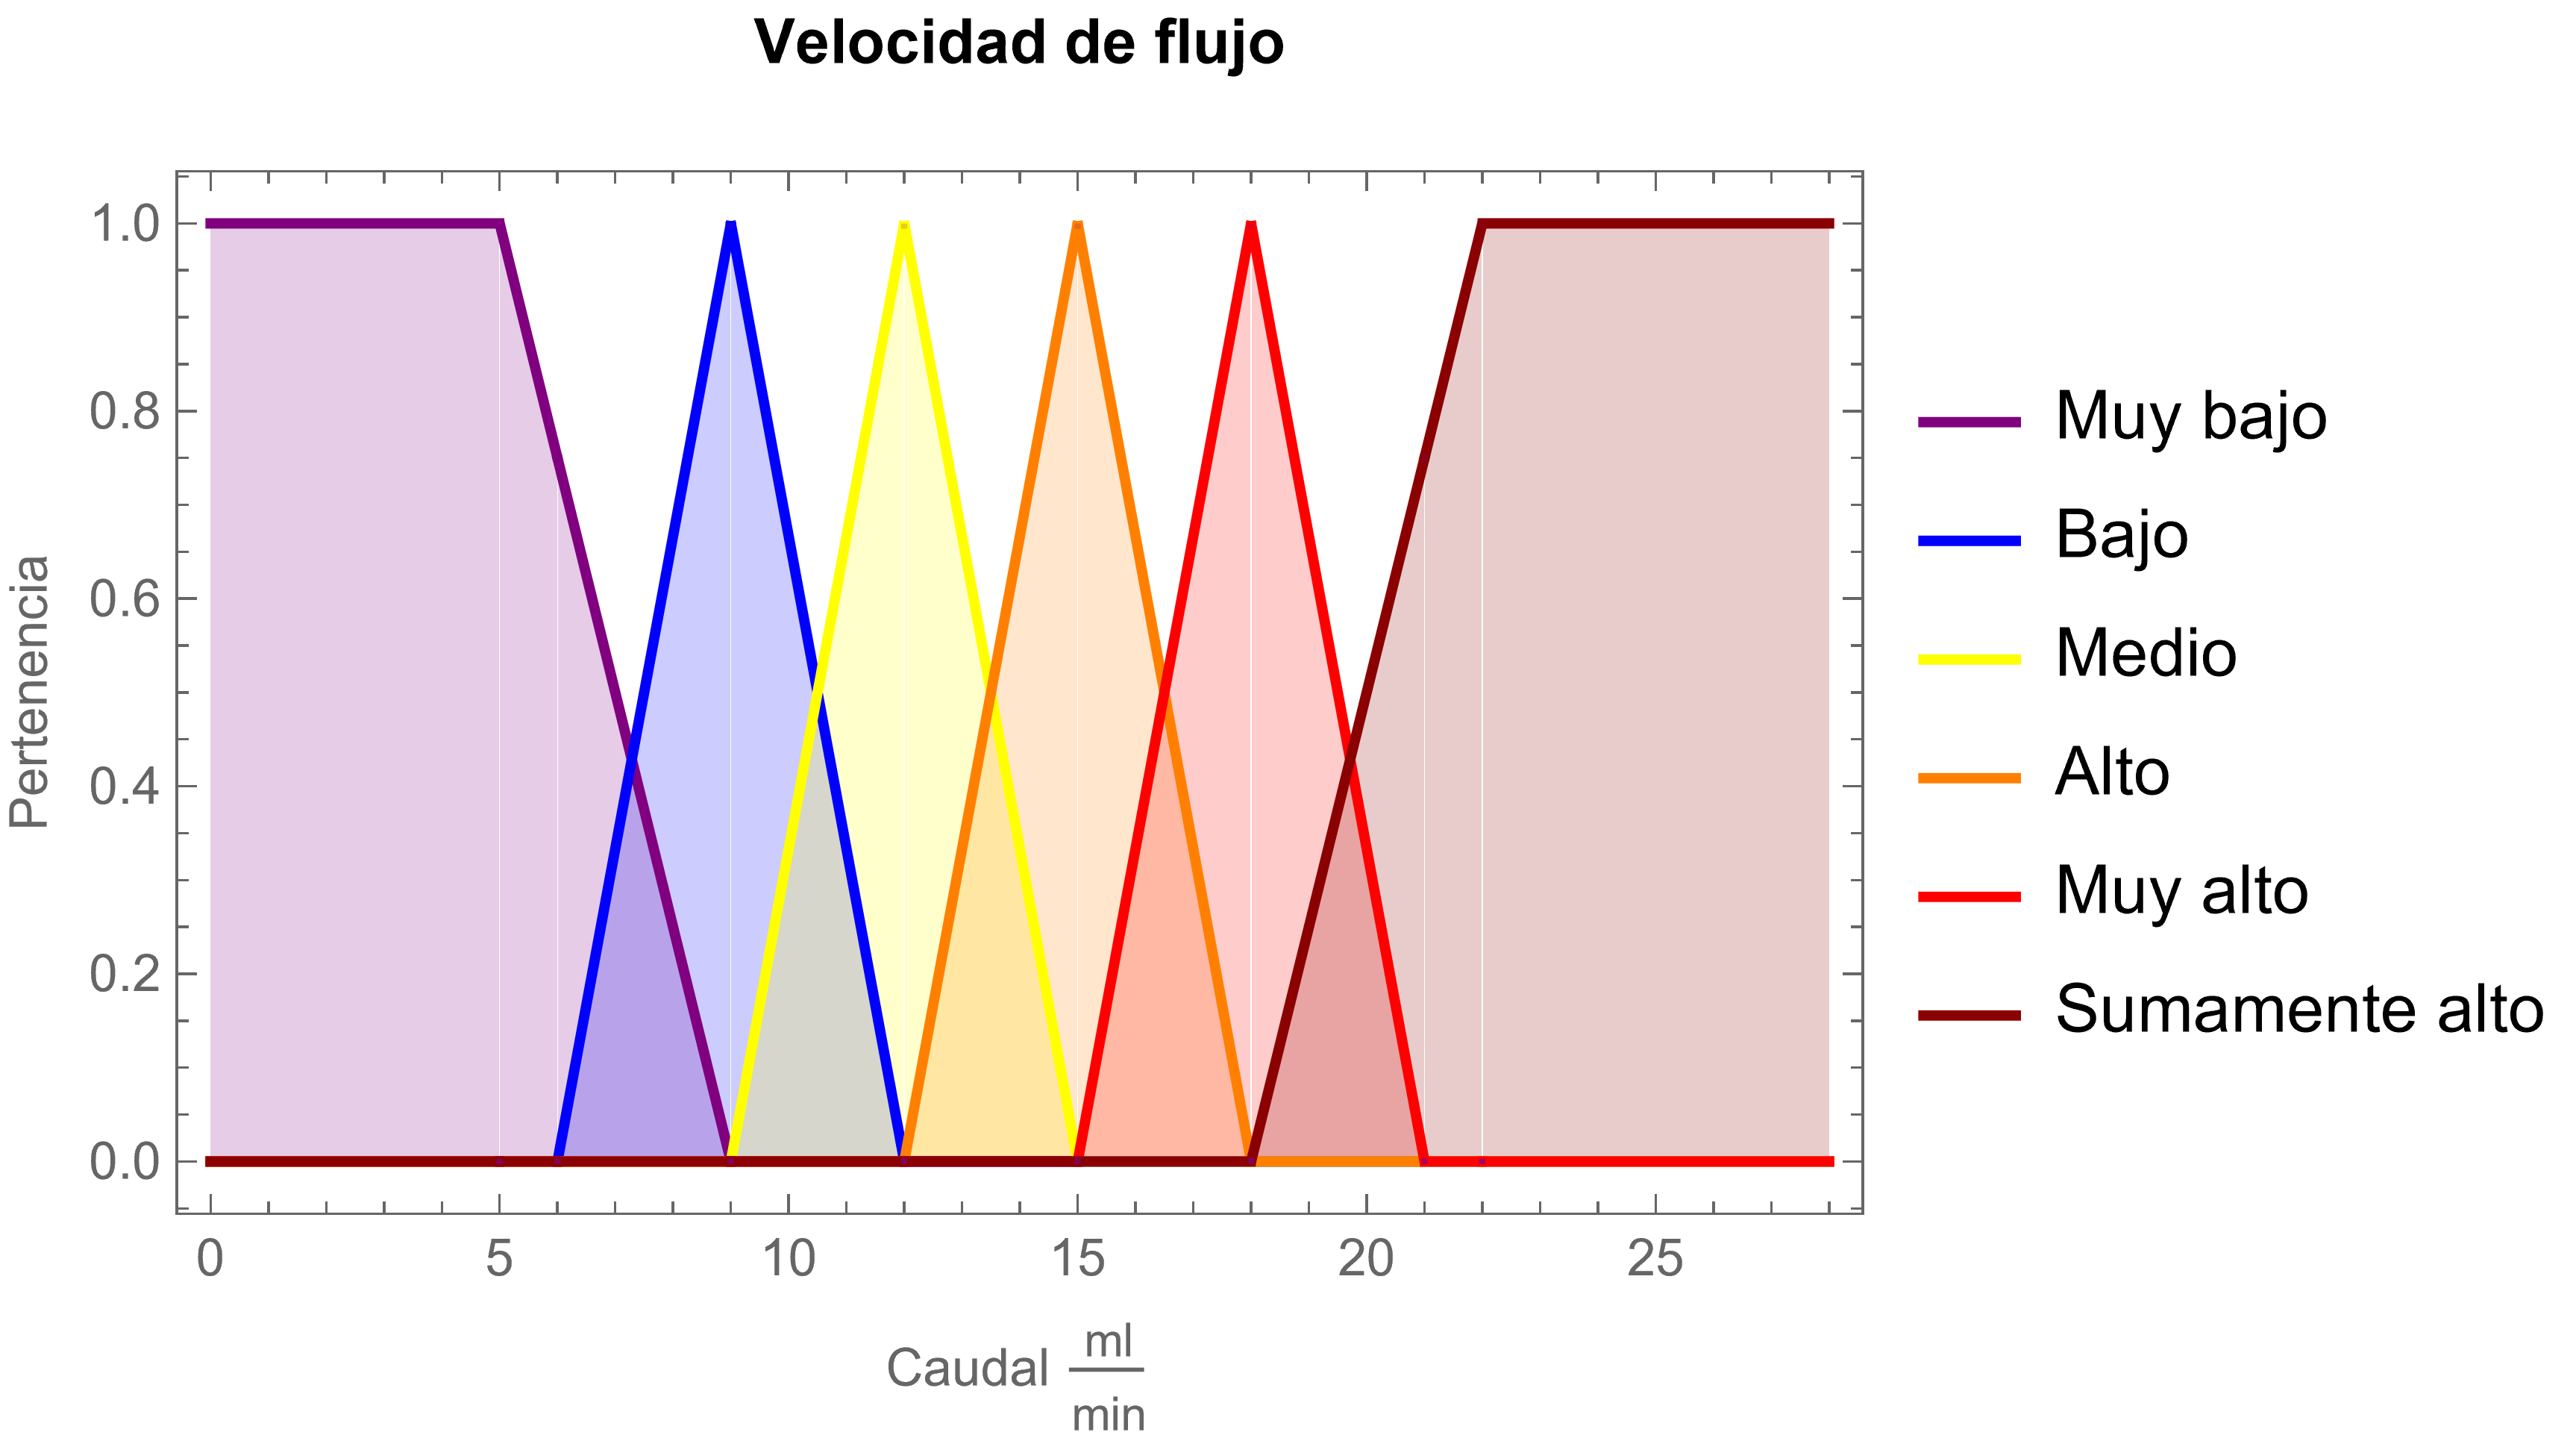
\includegraphics[
					width=\linewidth,
					height=65mm,
					keepaspectratio
				]{Resultados/Control/FlowVelocity.png}
				\caption{Funciones de membresía de la respuesta difusa.}
				\label{fig:FlowVelocity}
			\end{figure}
			
			Una vez llegado a este punto se definieron las reglas que rigen el sistema difuso. Para representarlas con un mayor orden se dividieron en bloques.
			
			\textit{Si la temperatura del recibidor solar es muy baja:}\par
			
			\begin{itemize}
				\item El caudal es nulo en todos los casos.
			\end{itemize}
			
			\textit{Si la temperatura del recibidor solar es baja:}\par
			\begin{itemize}
				\item Si la temperatura del recibidor solar es baja y además no es muy baja, y la temperatura del agua de entrada es muy alta, el caudal es medio
				\item Si la temperatura del recibidor solar es baja y además no es muy baja, y la temperatura del agua de entrada es alta, el caudal es bajo
				\item Si la temperatura del recibidor solar es baja y además no es muy baja, y la temperatura del agua de entrada es media, el caudal es muy bajo
			\end{itemize}
			
			\textit{Si la temperatura del recibidor solar es media:}\par
			\begin{itemize}
				\item Si la temperatura del recibidor solar es media y la temperatura del agua de entrada es muy baja, el caudal es muy bajo
				\item Si la temperatura del recibidor solar es media y la temperatura del agua de entrada es baja, el caudal es bajo
				\item Si la temperatura del recibidor solar es media y la temperatura del agua de entrada es media, el caudal es medio
				\item Si la temperatura del recibidor solar es media y la temperatura del agua de entrada es alta o muy alta, el caudal es alto
			\end{itemize}
			
			\textit{Si la temperatura del recibidor solar es alta:}\par
			\begin{itemize}
				\item Si la temperatura del recibidor solar es media o alta y la temperatura del agua de entrada es muy baja, el caudal es bajo.
				\item Si la temperatura del recibidor solar es media o alta y la temperatura del agua de entrada es baja, el caudal es medio
			\end{itemize}
			
			\textit{Si la temperatura del recibidor solar es muy alta:}\par
			\begin{itemize}
				\item Si la temperatura del recibidor solar es media pero no baja y la temperatura del agua de entrada es muy alta, el caudal es alto
				\item Si la temperatura del recibidor solar es media y la temperatura del agua de entrada es muy alta, el caudal es alto
				\item Si la temperatura del recibidor solar es alta y la temperatura del agua de entrada es muy alta o alta, el caudal es alto
				\item Si la temperatura del recibidor solar es muy alta y la temperatura del agua de entrada es muy alta o alta, el caudal es muy alto
			\end{itemize}
			
			Este conjunto de reglas tienen como objetivo tratar de mantener la temperatura del agua entre \qtyrange{60}{65}{\degreeCelsius} con el fin de evitar daños en los componentes eléctricos.
	
	
	\section{Construcción e integración del sistema}
		
		\section{Módulo de reaprovechamiento térmico y bombeo}
		
			El intercambiador de calor 
			
			\begin{figure}[H]
				\centering
				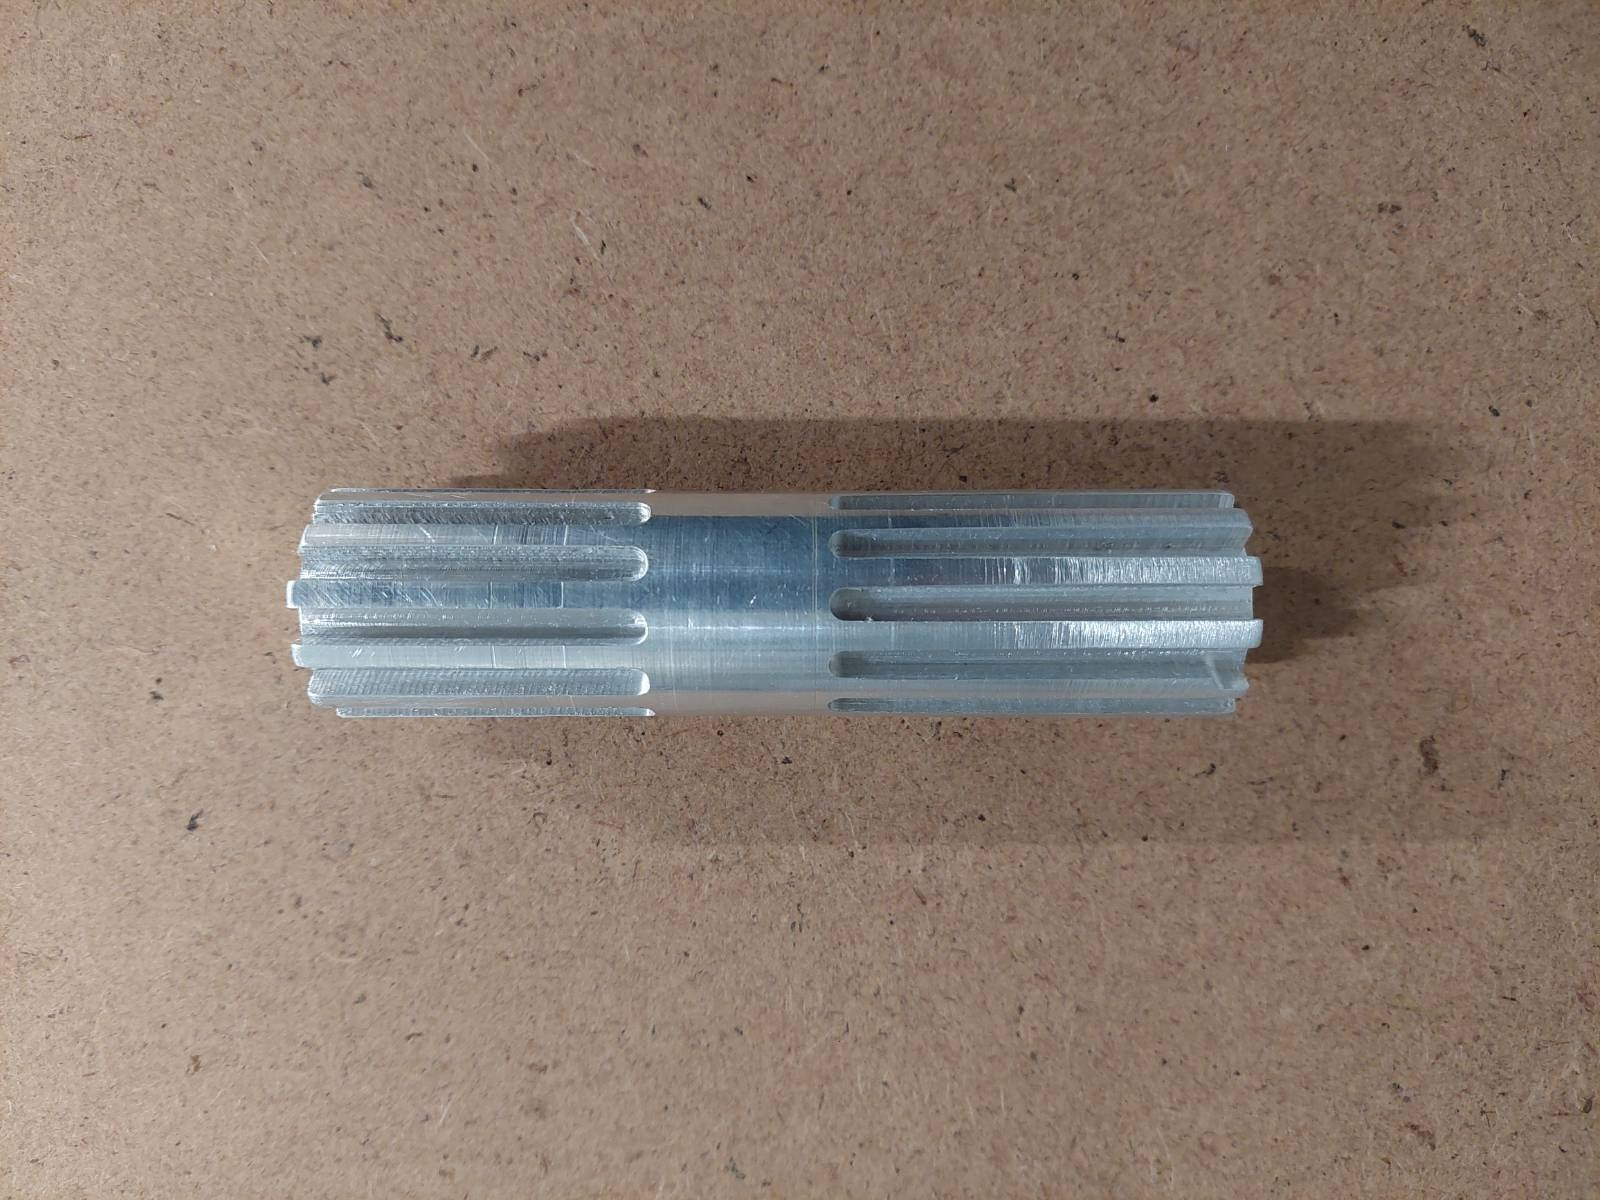
\includegraphics[
					width=\linewidth,
					height=65mm,
					keepaspectratio
				]{Resultados/Construcción/Intercambiador-de-calor.jpg}
				\caption{Intercambiador de calor con aletas verticales}
				\label{fig:Intercambiador-de-calor.jpeg}
			\end{figure}
		
	
	\section{Integración al seguidor solar}
	
		Para integrar el desalinizador al seguidor solar, se construyó un marco que soportara la lente, la altura de colocación de la lente se calculó mediante la ley de Snell y trigonometría siguiendo el arreglo mostrado en la~\cref{fig:DiagramaRayos}.
		
		\begin{figure}[H]
			\centering
			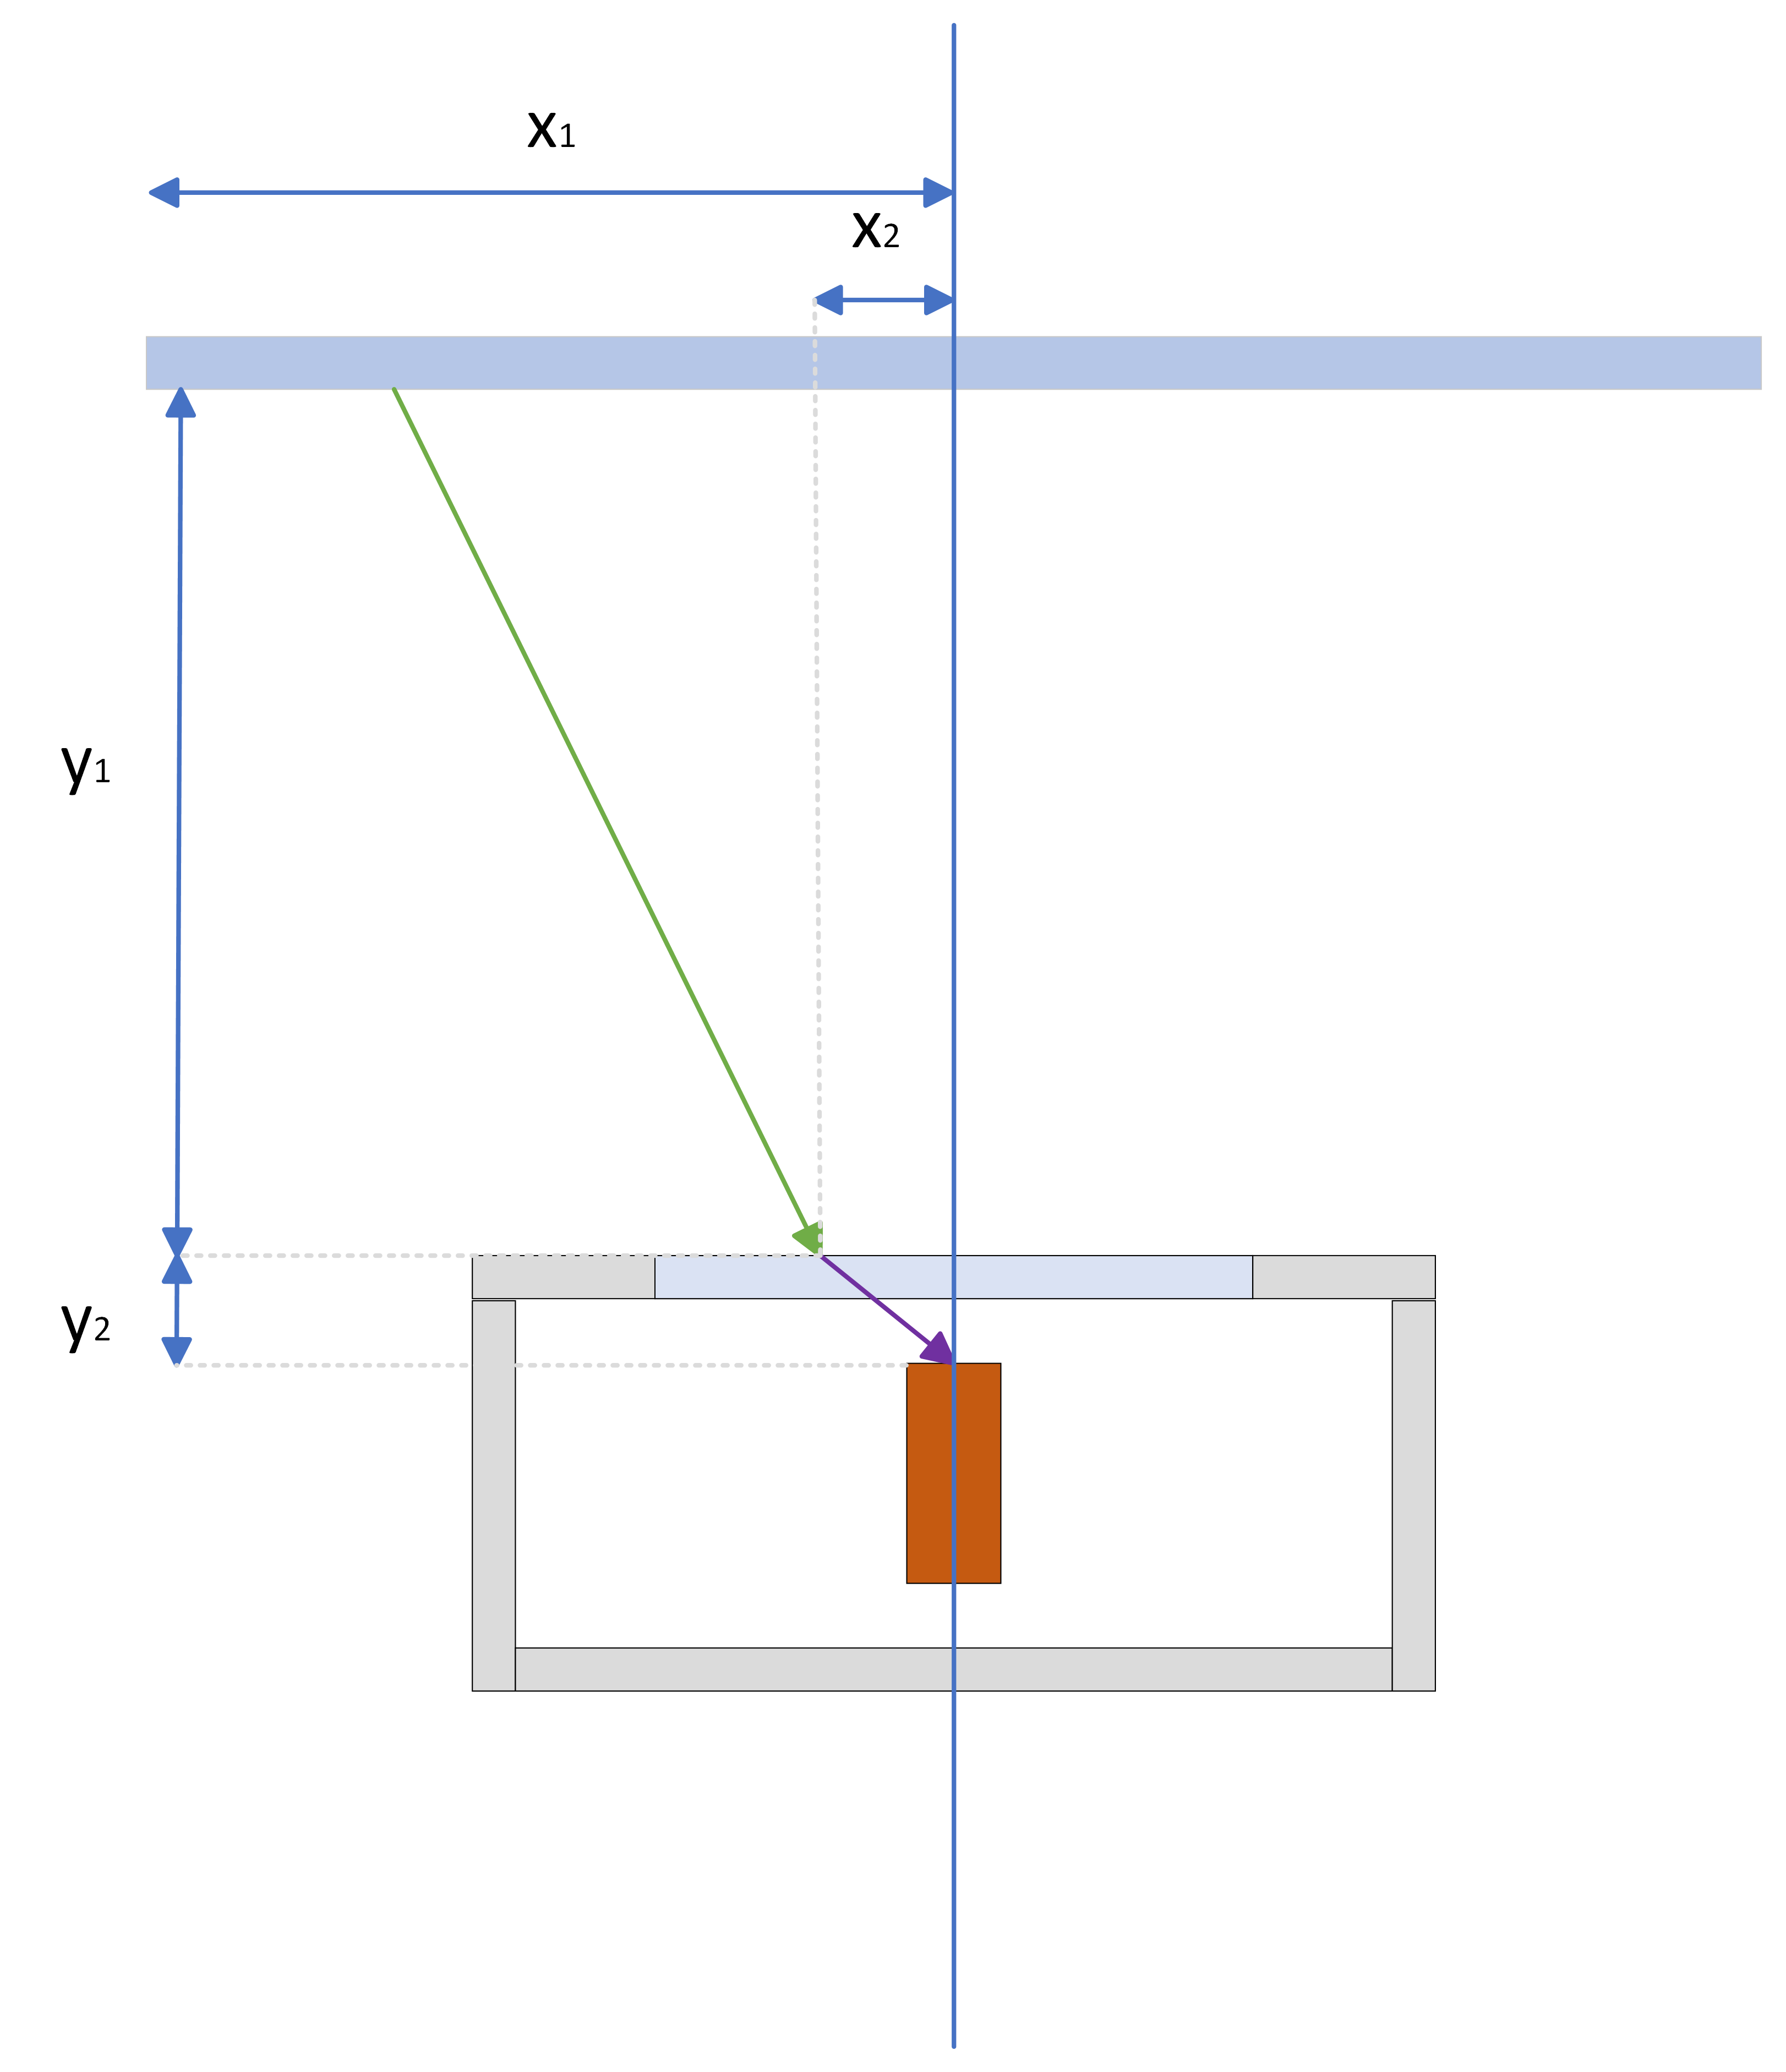
\includegraphics[
				width=\linewidth,
				height=65mm,
				keepaspectratio
			]{Resultados/Integración/DiagramaRayos.png}
			\caption{Trazado de rayos que permiten calcular la altura de la lente con respecto al punto focal.}
			\label{fig:DiagramaRayos}
		\end{figure}
		
		
		De los cálculos hechos, se obtuvo una altura al punto focal de \qty{362.45}{\mm}. A eso se le sumó la altura del recibidor solar con respecto al módulo de concentración solar dando que la altura mínima del marco es de \qty{442.50}{\mm}
		
			
			


			
			
			
			
	\input{Content/Chapter-8/DiscusiónDeResultados.tex}
	\printbibliography[heading=bibintoc]
	
	\appendix
	%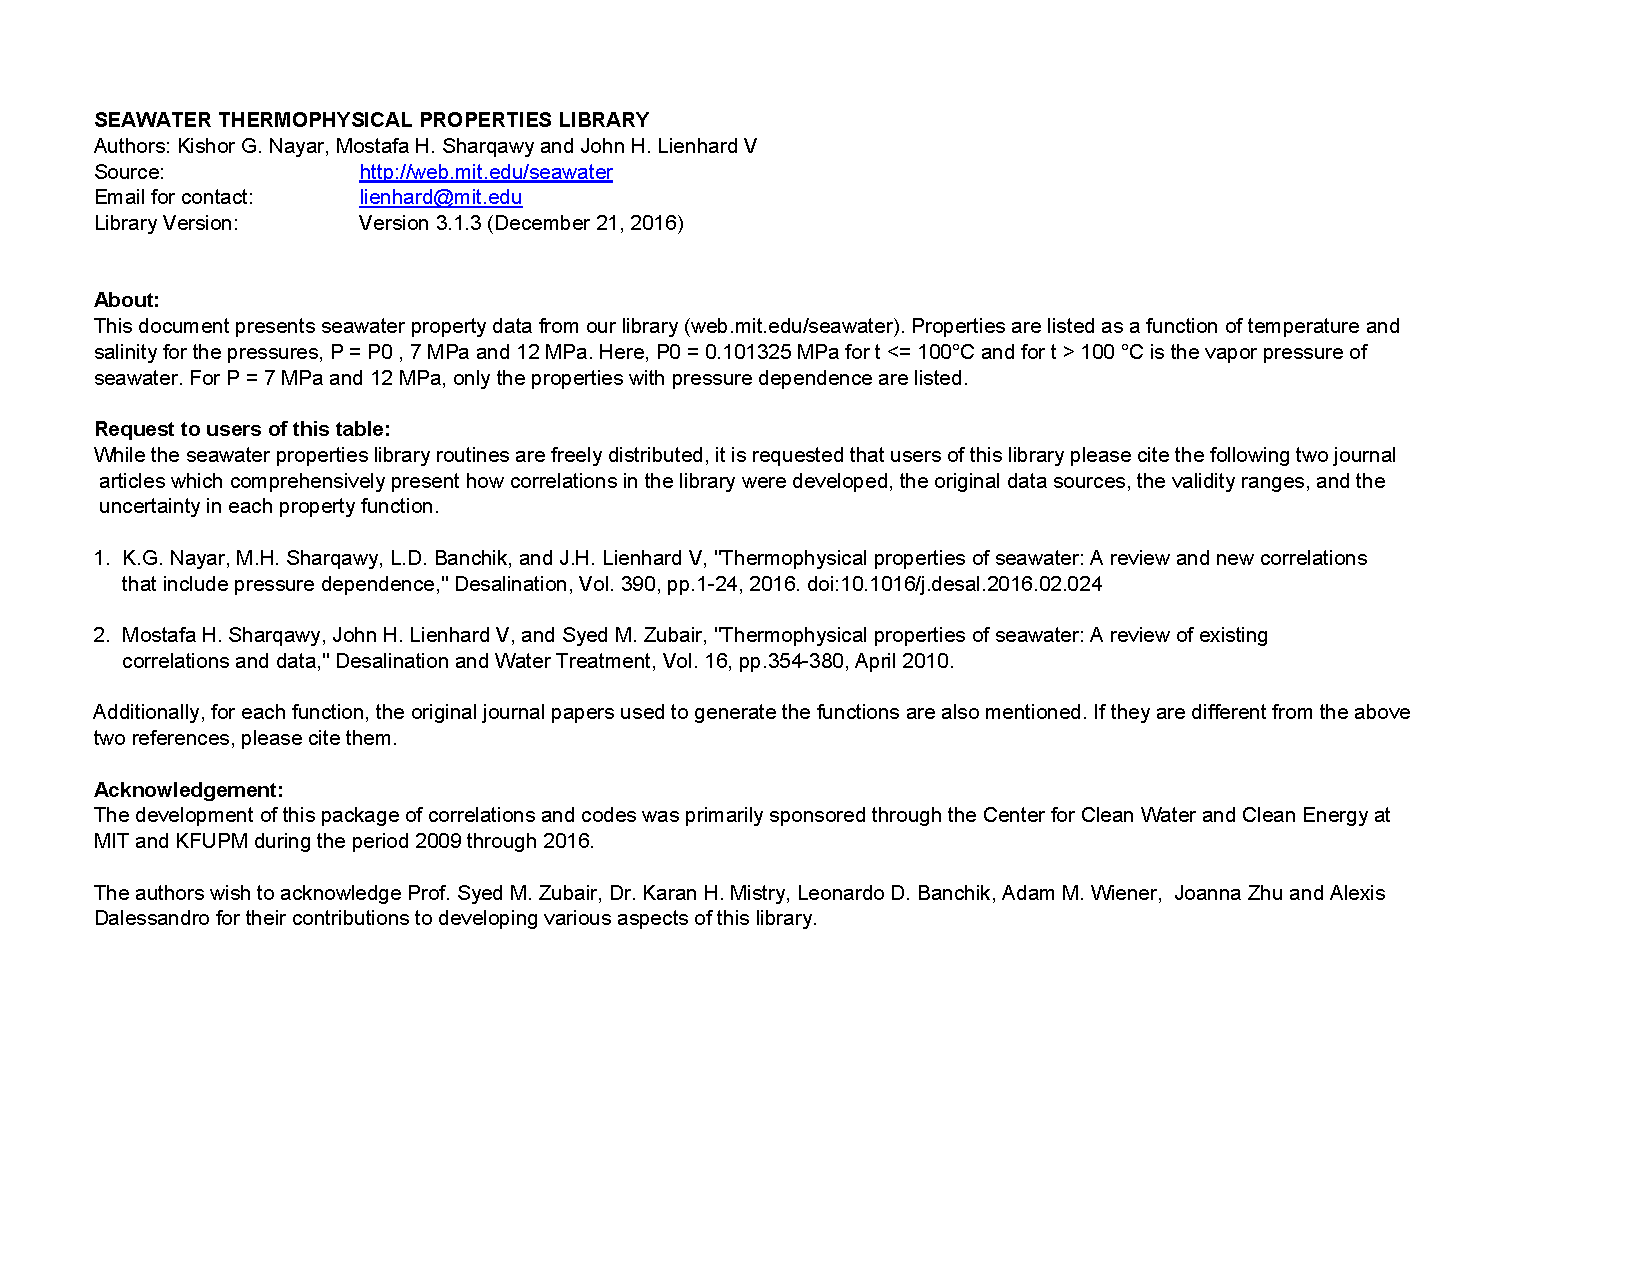
\includepdf[pages=1,pagecommand={\chapter{Propiedades del agua de mar}\label{ch:seawater-properties}\thispagestyle{generalfancy}}]{Content/Appendix/MIT_Seawater_Property_Tables_r2b.pdf}
%
%\includepdf[pages={4,12-13,15,25}, pagecommand={\thispagestyle{generalfancy}}]{Content/Appendix/MIT_Seawater_Property_Tables_r2b.pdf}

\chapter{Propiedades del agua de mar}\label{ch:seawater-properties}

Los datos mostrados en este apéndice son datos distribuidos gratuitamente  gracias a los siguientes artículos de revistas científicas \cites{nayar_thermophysical_2016}{sharqawy_thermophysical_2010}.

	Considerando \(
		P = \begin{cases}
			\qty{101.325}{\kilo\pascal} & \gls{T} \leq \qty{100}{\degreeCelsius} \\
			\text{Presión de vapor de agua} & \gls{T} > \qty{100}{\degreeCelsius} \\
		\end{cases}
	\) para las~\cref{table:Elevación-punto-ebullición,table:Conductividad-térmica-agua-salada,table:Calor-latente-vaporización}

\begin{longtblr}[
	caption = {Elevación del punto de ebullición según su salinidad},
	label = {table:Elevación-punto-ebullición},
	remark{Nota} = {El cambio de temperatura está dado en kelvin}
]{
	colspec = {*{13}{X[c]}},
	cell{1}{1} = {c = 13}{},
	row {1,2} = {
		bg = tabletitleblue,
		fg = white,
		font = \bfseries
	},
	row{even[3]} = {
		bg = tablerowblue
	},
	rowhead = 2,
	width = \linewidth,
	row{3-Z} = {
		font = \footnotesize
	}
}
	Salinidad\\
	{T $\left[\unit{\degreeCelsius}\right]$} 
		& 10 & 20 & 30 & 40 & 50 & 60 & 70 & 80 & 90 & 100 & 110 & 120 \\ 
        0 & 0.067 & 0.138 & 0.213 & 0.291 & 0.373 & 0.458 & 0.547 & 0.64 & 0.736 & 0.836 & 0.939 & 1.046 \\ 
        10 & 0.073 & 0.15 & 0.232 & 0.317 & 0.407 & 0.501 & 0.599 & 0.701 & 0.807 & 0.917 & 1.032 & 1.151 \\ 
        20 & 0.079 & 0.163 & 0.251 & 0.344 & 0.442 & 0.545 & 0.652 & 0.764 & 0.88 & 1.002 & 1.128 & 1.258 \\ 
        30 & 0.085 & 0.176 & 0.272 & 0.373 & 0.479 & 0.59 & 0.707 & 0.829 & 0.956 & 1.088 & 1.225 & 1.368 \\ 
        40 & 0.092 & 0.19 & 0.293 & 0.402 & 0.517 & 0.637 & 0.764 & 0.895 & 1.033 & 1.176 & 1.325 & 1.48 \\ 
        50 & 0.099 & 0.204 & 0.315 & 0.433 & 0.556 & 0.686 & 0.822 & 0.964 & 1.112 & 1.267 & 1.428 & 1.595 \\ 
        60 & 0.106 & 0.219 & 0.338 & 0.464 & 0.597 & 0.736 & 0.882 & 1.035 & 1.194 & 1.36 & 1.532 & 1.711 \\ 
        70 & 0.114 & 0.234 & 0.362 & 0.497 & 0.639 & 0.788 & 0.944 & 1.107 & 1.277 & 1.455 & 1.639 & 1.831 \\ 
        80 & 0.121 & 0.25 & 0.387 & 0.53 & 0.682 & 0.841 & 1.007 & 1.181 & 1.363 & 1.552 & 1.748 & 1.952 \\ 
        90 & 0.129 & 0.267 & 0.412 & 0.565 & 0.726 & 0.895 & 1.072 & 1.257 & 1.45 & 1.651 & 1.86 & 2.076 \\ 
        100 & 0.138 & 0.284 & 0.438 & 0.601 & 0.772 & 0.952 & 1.139 & 1.335 & 1.54 & 1.752 & 1.973 & 2.203 \\ 
        110 & 0.146 & 0.302 & 0.465 & 0.638 & 0.819 & 1.009 & 1.208 & 1.415 & 1.631 & 1.856 & 2.089 & 2.331 \\
\end{longtblr}

\begin{longtblr}[
	caption = {Conductividad térmica del agua según su salinidad},
	label = {table:Conductividad-térmica-agua-salada},
	remark{Nota} = {La conductividad está dada en \unit{\watt\per\m\kelvin}}
]{
	colspec = {*{13}{X[c]}},
	cell{1}{1} = {c = 13}{},
	rowhead = 2,
	row {1,2} = {
		bg = tabletitleblue,
		fg = white,
		font = \bfseries
	},
	row{even[3]} = {
		bg = tablerowblue
	},	
	width = \linewidth,
	row{3-Z} = {
		font = \footnotesize
	}
}
	Salinidad\\
	{T $\left[\unit{\degreeCelsius}\right]$} & 0 & 10 & 20 & 30 & 40 & 50 & 60 & 70 & 80 & 90 & 100 & 110 & 120 \\ 
	0 & 0.572 & 0.571 & 0.57 & 0.57 & 0.569 & 0.569 & 0.568 & 0.568 & 0.567 & 0.566 & 0.566 & 0.565 & 0.565 \\ 
	10 & 0.588 & 0.588 & 0.587 & 0.587 & 0.586 & 0.585 & 0.585 & 0.584 & 0.584 & 0.583 & 0.583 & 0.582 & 0.582 \\ 
	20 & 0.604 & 0.603 & 0.602 & 0.602 & 0.601 & 0.601 & 0.6 & 0.6 & 0.599 & 0.599 & 0.598 & 0.598 & 0.597 \\ 
	30 & 0.617 & 0.617 & 0.616 & 0.616 & 0.615 & 0.615 & 0.614 & 0.614 & 0.613 & 0.613 & 0.612 & 0.612 & 0.611 \\ 
	40 & 0.63 & 0.629 & 0.629 & 0.628 & 0.628 & 0.627 & 0.627 & 0.626 & 0.626 & 0.625 & 0.625 & 0.624 & 0.624 \\ 
	50 & 0.641 & 0.64 & 0.64 & 0.639 & 0.639 & 0.638 & 0.638 & 0.637 & 0.637 & 0.636 & 0.636 & 0.635 & 0.635 \\ 
	60 & 0.65 & 0.65 & 0.649 & 0.649 & 0.648 & 0.648 & 0.647 & 0.647 & 0.647 & 0.646 & 0.646 & 0.645 & 0.645 \\ 
	70 & 0.658 & 0.658 & 0.658 & 0.657 & 0.657 & 0.656 & 0.656 & 0.655 & 0.655 & 0.655 & 0.654 & 0.654 & 0.653 \\ 
	80 & 0.665 & 0.665 & 0.665 & 0.664 & 0.664 & 0.663 & 0.663 & 0.663 & 0.662 & 0.662 & 0.661 & 0.661 & 0.661 \\ 
	90 & 0.671 & 0.671 & 0.67 & 0.67 & 0.67 & 0.669 & 0.669 & 0.669 & 0.668 & 0.668 & 0.667 & 0.667 & 0.667 \\ 
	100 & 0.676 & 0.675 & 0.675 & 0.675 & 0.674 & 0.674 & 0.674 & 0.673 & 0.673 & 0.673 & 0.672 & 0.672 & 0.672 \\ 
	110 & 0.679 & 0.679 & 0.679 & 0.678 & 0.678 & 0.678 & 0.677 & 0.677 & 0.677 & 0.676 & 0.676 & 0.676 & 0.675 \\ 
	120 & 0.682 & 0.681 & 0.681 & 0.681 & 0.68 & 0.68 & 0.68 & 0.679 & 0.679 & 0.679 & 0.679 & 0.678 & 0.678 \\ 
\end{longtblr}


\begin{longtblr}[
	caption = {Calor latente de vaporización del agua según su salinidad},
	label = {table:Calor-latente-vaporización},
	remark{Nota} = {El calor latente de vaporización está dado en \unit{\kilo\joule\per\kg}}
]{
	colspec = {*{13}{X[c]}},
	cell{1}{1} = {c = 13}{},
	rowhead = 2,
	row {1,2} = {
		bg = tabletitleblue,
		fg = white,
		font = \bfseries
	},
	row{even[3]} = {
		bg = tablerowblue
	},	
	width = \linewidth,
	row{3-Z} = {
		font = \scriptsize
	}
}
	Salinidad\\
	{T $\left[\unit{\degreeCelsius}\right]$} & 0 & 10 & 20 & 30 & 40 & 50 & 60 & 70 & 80 & 90 & 100 & 110 & 120 \\ 
	0 & 2500.9 & 2475.9 & 2450.9 & 2425.9 & 2400.9 & 2375.9 & 2350.8 & 2325.8 & 2300.8 & 2275.8 & 2250.8 & 2225.8 & 2200.8 \\ 
	10 & 2477.2 & 2452.5 & 2427.7 & 2402.9 & 2378.1 & 2353.4 & 2328.6 & 2303.8 & 2279 & 2254.3 & 2229.5 & 2204.7 & 2180 \\ 
	20 & 2453.6 & 2429 & 2404.5 & 2379.9 & 2355.4 & 2330.9 & 2306.3 & 2281.8 & 2257.3 & 2232.7 & 2208.2 & 2183.7 & 2159.1 \\ 
	30 & 2429.8 & 2405.5 & 2381.2 & 2356.9 & 2332.6 & 2308.3 & 2284 & 2259.7 & 2235.4 & 2211.1 & 2186.8 & 2162.5 & 2138.2 \\ 
	40 & 2406 & 2381.9 & 2357.9 & 2333.8 & 2309.7 & 2285.7 & 2261.6 & 2237.6 & 2213.5 & 2189.4 & 2165.4 & 2141.3 & 2117.3 \\ 
	50 & 2382 & 2358.1 & 2334.3 & 2310.5 & 2286.7 & 2262.9 & 2239 & 2215.2 & 2191.4 & 2167.6 & 2143.8 & 2120 & 2096.1 \\ 
	60 & 2357.7 & 2334.1 & 2310.5 & 2287 & 2263.4 & 2239.8 & 2216.2 & 2192.7 & 2169.1 & 2145.5 & 2121.9 & 2098.3 & 2074.8 \\ 
	70 & 2333.1 & 2309.8 & 2286.4 & 2263.1 & 2239.8 & 2216.4 & 2193.1 & 2169.8 & 2146.4 & 2123.1 & 2099.8 & 2076.5 & 2053.1 \\ 
	80 & 2308.1 & 2285 & 2261.9 & 2238.8 & 2215.8 & 2192.7 & 2169.6 & 2146.5 & 2123.4 & 2100.4 & 2077.3 & 2054.2 & 2031.1 \\ 
	90 & 2282.6 & 2259.7 & 2236.9 & 2214.1 & 2191.3 & 2168.4 & 2145.6 & 2122.8 & 2100 & 2077.1 & 2054.3 & 2031.5 & 2008.7 \\ 
	100 & 2256.5 & 2233.9 & 2211.3 & 2188.8 & 2166.2 & 2143.7 & 2121.1 & 2098.5 & 2076 & 2053.4 & 2030.8 & 2008.3 & 1985.7 \\ 
	110 & 2229.7 & 2207.4 & 2185.1 & 2162.8 & 2140.5 & 2118.2 & 2095.9 & 2073.6 & 2051.3 & 2029 & 2006.7 & 1984.4 & 1962.1 \\ 
	120 & 2202.1 & 2180.1 & 2158.1 & 2136.1 & 2114.1 & 2092 & 2070 & 2048 & 2026 & 2003.9 & 1981.9 & 1959.9 & 1937.9 \\ 
\end{longtblr}

\begin{figure}[H]
	\centering
	\begin{subfigure}{0.45\linewidth}
		\centering
		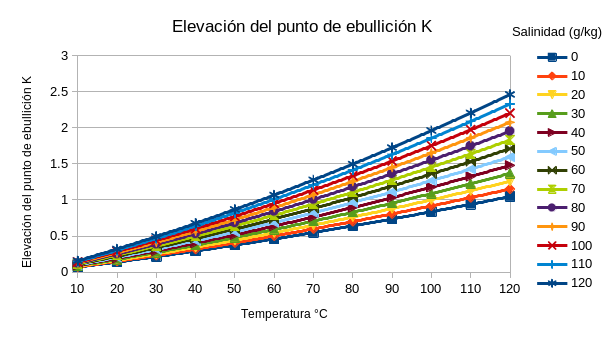
\includegraphics[width=\linewidth, keepaspectratio]{Apéndices/Elevación-punto-ebullición.png}
		\caption{Elevación del punto de ebullición según aumenta la salinidad del agua (\cref{table:Elevación-punto-ebullición})}
		\label{fig:Elevación-punto-ebullición}
	\end{subfigure}
	\hfill
	\begin{subfigure}{0.45\linewidth}
		\centering
		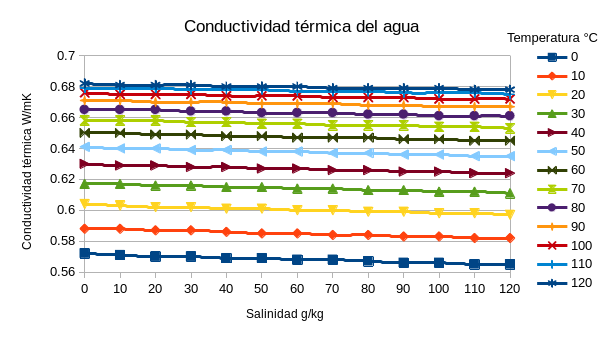
\includegraphics[width=\linewidth, keepaspectratio]{Apéndices/Conductividad-térmica-agua.png}
		\caption{Disminución de la conductividad térmica según aumenta la salinidad del agua (\cref{table:Conductividad-térmica-agua-salada})}
		\label{fig:Conductividad-térmica-agua}
	\end{subfigure}
	\caption{Gráficas del~\cref{ch:seawater-properties}}
	\label{fig:graficas-propiedades-agua-salinidad}
\end{figure}	
	\chapter{Propiedades del agua saturada}\label{ch:agua-saturada-propiedades}
	
	\begin{longtblr}[
		caption = {Propiedades del agua saturada},
		label = {table:propiedades-agua-sat},
		remark{Fuente} = {\fullcite{cengel_fluid_2006}}
	]{
		colspec = {*{1}{X[0.5]} *{4}{X[c]} *{2}{X[0.75]} *{2}{X[c]} *{3}{X[1.5]}},
		rows = {
			halign = c,
			valign = m
		},
		stretch = 0,
		row {1,2} = {
			bg = tabletitleblue,
			fg = white,
			font = \tiny\bfseries
		},
		row{even[3]} = {
			bg = tablerowblue
		},
		rowhead = 3,
		width = \linewidth,
		row{3-Z} = {
			font = \tiny
		},
		cell{1-2}{3,6,8,10} = {c=2}{}
	}
		T.
			& {P. de\\Sat.}
			& Densidad &
			& {Entalpía\\de\\vap.}
			& $C_{s}$ &
			& {Conductividad\\térmica} &
			& {Viscosidad\\dinámica} &
			& {C. de expansión\\Volumétrica}\\
		\unit{\degreeCelsius}
			& \unit{\kilo\pascal}
			& \unit{\kilogram\per\m\tothe{3}} &
			& \unit{\kilo\joule\per\kg}
			& \unit{\joule\per\kg\kelvin} &
			& \unit{\watt\per\m\kelvin} &
			& \unit{\kilogram\per\m\s} &
			& \unit{\per\kelvin}
		\\
		---
			& ---
			& Líquido
			& Vapor
			& ---
			& Líquido
			& Vapor
			& Líquido
			& Vapor
			& Líquido
			& Vapor
			& Líquido\\
		\num{0.01} 
			& \num{0.6113}
			& \num{999.8}
			& \num{0.0048}
			& \num{2501}
			& \num{4217}
			& \num{1854}
			& \num{0.561}
			& \num{0.0171}
			& \num{1.792e-3}
			& \num{0.922e-5}
			& \num{-0.068e-3} \\
		\num{5}
			& \num{0.8721}
			& \num{999.9}
			& \num{0.0068} 
			& \num{2490} 
			& \num{4205} 
			& \num{1857} 
			& \num{0.571} 
			& \num{0.0173} 
			& \num{1.519e-3} 
			& \num{0.934e-5}
			& \num{0.015e-3} \\
		\num{10} 
			& \num{1.2276} 
			& \num{999.7} 
			& \num{0.0094} 
			& \num{2478} 
			& \num{4194} 
			& \num{1862} 
			& \num{0.58} 
			& \num{0.0176} 
			& \num{1.307e-3} 
			& \num{0.946e-5} 
			& \num{0.733e-3} \\
        \num{15} 
			& \num{1.7051} 
			& \num{999.1} 
			& \num{0.0128} 
			& \num{2466} 
			& \num{4186} 
			& \num{1863} 
			& \num{0.589} 
			& \num{0.0179} 
			& \num{1.138e-3} 
			& \num{0.959e-5} 
			& \num{0.138e-3} \\
        \num{20} 
			& \num{2.339} 
			& \num{998} 
			& \num{0.0173} 
			& \num{2454} 
			& \num{4182} 
			& \num{1867} 
			& \num{0.598} 
			& \num{0.0182} 
			& \num{1.002e-3} 
			& \num{0.973e-5} 
			& \num{0.195e-3} \\
        \num{25} 
			& \num{3.169} 
			& \num{997} 
			& \num{0.0231} 
			& \num{2442} 
			& \num{4180} 
			& \num{1870} 
			& \num{0.607} 
			& \num{0.0186} 
			& \num{0.891e-3} 
			& \num{0.987e-5} 
			& \num{0.247e-3} \\
		\num{30} 
			& \num{4.246} 
			& \num{996} 
			& \num{0.0304} 
			& \num{2431} 
			& \num{4178} 
			& \num{1875} 
			& \num{0.615} 
			& \num{0.0189} 
			& \num{0.798e-3} 
			& \num{1.001e-5}
			& \num{0.294e-3} \\
        \num{35} 
			& \num{5.628} 
			& \num{994} 
			& \num{0.0397} 
			& \num{2419} 
			& \num{4178} 
			& \num{1880} 
			& \num{0.623} 
			& \num{0.0192} 
			& \num{0.720e-3} 
			& \num{1.016e-5}
			& \num{0.337e-3} \\
        \num{40} 
			& \num{7.384} 
			& \num{992.1} 
			& \num{0.0512} 
			& \num{2407} 
			& \num{4179} 
			& \num{1885} 
			& \num{0.631} 
			& \num{0.0196} 
			& \num{0.653e-3} 
			& \num{1.031e-5}
			& \num{0.377e-3} \\
        \num{45} 
			& \num{9.593} 
			& \num{990.1} 
			& \num{0.0655} 
			& \num{2395} 
			& \num{4180} 
			& \num{1892} 
			& \num{0.637} 
			& \num{0.02} 
			& \num{0.596e-3} 
			& \num{1.046e-5}
			& \num{0.415e-3} \\
        \num{50} 
			& \num{12.35} 
			& \num{988.1} 
			& \num{0.0831} 
			& \num{2383} 
			& \num{4181} 
			& \num{1900} 
			& \num{0.644} 
			& \num{0.0204} 
			& \num{0.547e-3} 
			& \num{1.062e-5}
			& \num{0.451e-3} \\
		\num{55} 
			& \num{15.76} 
			& \num{985.2} 
			& \num{0.1045} 
			& \num{2371} 
			& \num{4183} 
			& \num{1908} 
			& \num{0.649} 
			& \num{0.0208} 
			& \num{0.504e-3} 
			& \num{1.077e-5}
			& \num{0.484e-3} \\
        \num{60} 
			& \num{19.94} 
			& \num{983.3} 
			& \num{0.1304} 
			& \num{2359} 
			& \num{4185} 
			& \num{1916} 
			& \num{0.654} 
			& \num{0.0212} 
			& \num{0.467e-3} 
			& \num{1.093e-5}
			& \num{0.517e-3} \\
        \num{65} 
			& \num{25.03} 
			& \num{980.4} 
			& \num{0.1614} 
			& \num{2346} 
			& \num{4187} 
			& \num{1926} 
			& \num{0.659} 
			& \num{0.0216} 
			& \num{0.433e-3} 
			& \num{1.110e-5}
			& \num{0.548e-3} \\
        \num{70} 
			& \num{31.19} 
			& \num{977.5} 
			& \num{0.1983} 
			& \num{2334} 
			& \num{4190} 
			& \num{1936} 
			& \num{0.663} 
			& \num{0.0221} 
			& \num{0.404e-3} 
			& \num{1.126e-5}
			& \num{0.578e-3} \\
        \num{75} 
			& \num{38.58} 
			& \num{974.7} 
			& \num{0.2421} 
			& \num{2321} 
			& \num{4193} 
			& \num{1948} 
			& \num{0.667} 
			& \num{0.0225} 
			& \num{0.378e-3} 
			& \num{1.142e-5}
			& \num{0.607e-3} \\
		\num{80} 
			& \num{47.39} 
			& \num{971.8} 
			& \num{0.2935} 
			& \num{2309} 
			& \num{4197} 
			& \num{1962} 
			& \num{0.67} 
			& \num{0.023} 
			& \num{0.355e-3} 
			& \num{1.159e-5}
			& \num{0.653e-3} \\
        \num{85} 
			& \num{57.83} 
			& \num{968.1} 
			& \num{0.3536} 
			& \num{2296} 
			& \num{4201} 
			& \num{1977} 
			& \num{0.673} 
			& \num{0.0235} 
			& \num{0.333e-3} 
			& \num{1.176e-5}
			& \num{0.670e-3} \\
        \num{90} 
			& \num{70.14} 
			& \num{965.3} 
			& \num{0.4235} 
			& \num{2283} 
			& \num{4206} 
			& \num{1993} 
			& \num{0.675} 
			& \num{0.024} 
			& \num{0.315e-3} 
			& \num{1.193e-5}
			& \num{0.702e-3} \\
		\num{95} 
			& \num{84.55} 
			& \num{961.5}
			& \num{0.5045}
			& \num{2270} 
			& \num{4212} 
			& \num{2010} 
			& \num{0.677} 
			& \num{0.0246} 
			& \num{0.297e-3}
			& \num{1.210e-5}
			& \num{0.716e-3}  \\
        \num{100} 
			& \num{101.33} 
			& \num{957.9} 
			& \num{0.5978} 
			& \num{2257} 
			& \num{4217} 
			& \num{2029} 
			& \num{0.679} 
			& \num{0.0251} 
			& \num{0.282e-3} 
			& \num{1.227e-5}
			& \num{0.750e-3} \\
        \num{110} 
			& \num{143.27} 
			& \num{950.6} 
			& \num{0.8263} 
			& \num{2230} 
			& \num{4229} 
			& \num{2071} 
			& \num{0.682} 
			& \num{0.0262} 
			& \num{0.255e-3} 
			& \num{1.261e-5}
			& \num{0.798e-3} \\
        \num{120} 
			& \num{198.53} 
			& \num{943.4} 
			& \num{1.121} 
			& \num{2203} 
			& \num{4244} 
			& \num{2120} 
			& \num{0.683} 
			& \num{0.0275} 
			& \num{0.232e-3} 
			& \num{1.296e-5}
			& \num{0.858e-3} \\
        \num{130} 
			& \num{270.1} 
			& \num{934.6} 
			& \num{1.496} 
			& \num{2174} 
			& \num{4263} 
			& \num{2177} 
			& \num{0.684} 
			& \num{0.0288} 
			& \num{0.213e-3} 
			& \num{1.330e-5}
			& \num{0.913e-3} \\
		\num{140} 
			& \num{361.3} 
			& \num{921.7} 
			& \num{1.965} 
			& \num{2145} 
			& \num{4286} 
			& \num{2244} 
			& \num{0.683} 
			& \num{0.0301} 
			& \num{0.197e-3} 
			& \num{1.365e-5}
			& \num{0.970e-3} \\
        \num{150} 
			& \num{475.8} 
			& \num{916.6} 
			& \num{2.546} 
			& \num{2114} 
			& \num{4311} 
			& \num{2314} 
			& \num{0.682} 
			& \num{0.0316} 
			& \num{0.183e-3} 
			& \num{1.399e-5}
			& \num{1.025e-3} \\
		\num{160} 
			& \num{617.8} 
			& \num{907.4} 
			& \num{3.256} 
			& \num{2083} 
			& \num{4340} 
			& \num{2420} 
			& \num{0.68} 
			& \num{0.0331} 
			& \num{0.170e-3} 
			& \num{1.434e-5}
			& \num{1.145e-3} \\
        \num{170} 
			& \num{791.7} 
			& \num{897.7} 
			& \num{4.119} 
			& \num{2050} 
			& \num{4370} 
			& \num{2490} 
			& \num{0.677} 
			& \num{0.0347} 
			& \num{0.160e-3} 
			& \num{1.468e-5}
			& \num{1.178e-3} \\
        \num{180} 
			& \num{1002.1} 
			& \num{887.3} 
			& \num{5.153} 
			& \num{2015} 
			& \num{4410} 
			& \num{2590} 
			& \num{0.673} 
			& \num{0.0364} 
			& \num{0.150e-3} 
			& \num{1.502e-5}
			& \num{1.210e-3}\\
        \num{190} 
			& \num{1254.4} 
			& \num{876.4} 
			& \num{6.388} 
			& \num{1979} 
			& \num{4460} 
			& \num{2710} 
			& \num{0.669} 
			& \num{0.0382} 
			& \num{0.142e-3} 
			& \num{1.537e-5}
			& \num{1.280e-3} \\
		\num{200} 
			& \num{1553.8} 
			& \num{864.3} 
			& \num{7852} 
			& \num{1941} 
			& \num{4500} 
			& \num{2840} 
			& \num{0.663} 
			& \num{0.0401} 
			& \num{0.134e-3} 
			& \num{1.571e-5}
			& \num{1.350e-3} \\
        \num{220} 
			& \num{2318} 
			& \num{840.3} 
			& \num{11.6} 
			& \num{1859} 
			& \num{4610} 
			& \num{3110} 
			& \num{0.65} 
			& \num{0.0442} 
			& \num{0.122e-3} 
			& \num{1.641e-5}
			& \num{1.520e-3} \\
        \num{240} 
			& \num{3344} 
			& \num{813.7} 
			& \num{16.73} 
			& \num{1767} 
			& \num{4760} 
			& \num{3520} 
			& \num{0.632} 
			& \num{0.0487} 
			& \num{0.111e-3} 
			& \num{1.712e-5}
			& \num{1.720e-3} \\
		\num{260} 
			& \num{4688} 
			& \num{783.7} 
			& \num{23.69} 
			& \num{1663} 
			& \num{4970} 
			& \num{4070} 
			& \num{0.609} 
			& \num{0.054} 
			& \num{0.102e-3} 
			& \num{1.788e-5}
			& \num{2.000e-3}\\
        \num{280} 
			& \num{6412} 
			& \num{750.8} 
			& \num{33.15} 
			& \num{1544} 
			& \num{5280} 
			& \num{4835} 
			& \num{0.581} 
			& \num{0.0605} 
			& \num{0.094e-3} 
			& \num{1.870e-5}
			& \num{2.380e-3} \\
        \num{300} 
			& \num{8581} 
			& \num{713.8} 
			& \num{46.15} 
			& \num{1405} 
			& \num{5750} 
			& \num{5980} 
			& \num{0.548} 
			& \num{0.0695} 
			& \num{0.086e-3} 
			& \num{1.965e-5}
			& \num{2.950e-3}
	\end{longtblr}


	\chapter{Código en jupyter julia para analizar las condiciones de la energía solar térmica en la CDMX}
\label{ch:solar-irradiation-code}

\section*{Paquetes importados}

\begin{lstlisting}
using Pkg
Pkg.add("Plots")
Pkg.add("HTTP")
Pkg.add("CategoricalArrays")
Pkg.add("DataFrames")
Pkg.add("CSV")
Pkg.add("Missings")
Pkg.add("Statistics")

using HTTP
using DataFrames
using CSV
using CategoricalArrays
using Missings
using Statistics
using Plots
\end{lstlisting}

\section*{Declaración de diccionarios}

\begin{lstlisting}
parameters = Dict(
	"hourly" => [
		"PS",
		"WS2M",
		"QV2M",
		"CLRSKY_SFC_SW_DWN",
		"ALLSKY_SFC_SW_DWN",
		"CLOUD_AMT",
		"ALLSKY_SFC_UVA",
		"ALLSKY_SFC_UVB"
	]
);

descriptions = Dict(
	"PS" => [
		"Surface Pressure",
		"The average of surface pressure at the surface of the earth.",
		"kPa"
	],
	"WS2M" => [
		"Wind Speed at 2 Meters",
		"The average of wind speed at 2 meters above the surface of the earth.",
		"m/s"
	],
	"QV2M" => [
		"Specific Humidity at 2 Meters",
		"The ratio of the mass of water vapor to the total mass of air at 2 meters (kg water/kg total air).",
		"g/kg"
	],
	"CLRSKY_SFC_SW_DWN" => [
		"Clear Sky Surface Shortwave Downward Irradiance",
		"""The total solar irradiance incident (direct plus diffuse) on a horizontal plane at the surface of the earth under clear sky conditions. An alternative term for the total solar irradiance is the "Global Horizontal Irradiance" or GHI.""",
		"Whr/m^2"
	],
	"ALLSKY_SFC_SW_DWN" => [
		"All Sky Surface Shortwave Downward Irradiance",
		"""The total solar irradiance incident (direct plus diffuse) on a horizontal plane at the surface of the earth under all sky conditions. An alternative term for the total solar irradiance is the "Global Horizontal Irradiance" or GHI.""",
		"Whr/m^2"
	],
	"CLOUD_AMT" => [
		"Cloud Amount",
		"The average percent of cloud amount during the temporal period.",
		"%"
	],
	"ALLSKY_SFC_UVA" => [
		"All Sky Surface UVA Irradiance",
		"The ultraviolet A (UVA 315nm-400nm) irradiance under all sky conditions.",
		"W/m^2"
	],
	"ALLSKY_SFC_UVB" => [
		"All Sky Surface UVB Irradiance",
		"The ultraviolet B (UVB 280nm-315nm) irradiance under all sky conditions.",
		"W/m^2"
	]
);

months = Dict(
	1 => "Enero",
	2 => "Febrero",
	3 => "Marzo",
	4 => "Abril",
	5 => "Mayo",
	6 => "Junio",
	7 => "Julio",
	8 => "Agosto",
	9 => "Septiembre",
	10 => "Octubre",
	11 => "Noviembre",
	12 => "Diciembre"
);
\end{lstlisting}

\section*{Constantes para la construcción de la URL}

\begin{lstlisting}
const LATITUDE::Float64 = 19.3038;
const LONGITUDE::Float64 = -99.0732;
START_DATE::Int64 = 20180101;
END_DATE::Int64 = 20221231;
\end{lstlisting}

\section*{Constantes}

\begin{lstlisting}
START_HOUR::Int64 = 4;
END_HOUR::Int64 = 18;
\end{lstlisting}

\section*{Solicitud de datos a la base de datos Power Larc de la NASA}

\begin{lstlisting}
path = joinpath(pwd(), "files");
if !isdir(path)
	mkdir(path)
end
for key in keys(parameters)
	URL::String = string(
		"https://power.larc.nasa.gov/api/temporal/$key/point",
		"?parameters=",
		join(parameters[key], ","),
		"&community=RE",
		"&longitude=$LONGITUDE",
		"&latitude=$LATITUDE",
		"&start=$START_DATE",
		"&end=$END_DATE",
		"&format=CSV"
	);
	download(URL, joinpath(path, "$START_DATE-$END_DATE-$key.csv"))
end
\end{lstlisting}

\section*{Tratamiento y análisis de datos}

Nota: Se confía en la fuente, por lo que se asume que no existen valores nulos en el DataFrame. Sin embargo, se observa que hay valores para rellenar iguales a -999. Se observa que estos valores son consecutivos a partir del 01/04/2022. Se espera que sea debido al periodo de recolección que pasa de ser cada hora a diario. Se buscará entonces otro dataset. Se encontró que en efecto, desde esa fecha no hay datos, aunque al corregirlo a diario, se reduce de 5 a 3 columnas la falta de datos, aunque aún se observan algunos datos faltantes.

\begin{lstlisting}
na_val = -999;
min_year::Int64 = trunc(Int, (START_DATE/10000));
max_year::Int64 = trunc(Int, (END_DATE/10000));
graphs_path = joinpath(pwd(), "graphs");
if !isdir(graphs_path)
	mkdir(graphs_path)
end

for file in readdir(path)
	df = DataFrame(CSV.File(joinpath(path, file), header=17))
	subset!(
		df,
		names(df) .=> ByRow(x -> x != na_val),
		:HR => ByRow(x -> x >= START_HOUR && x <= END_HOUR),
		:YEAR => ByRow(x -> x >= min_year)
	)

	if (isequal(file[19:end-4], "hourly"))
		gd = groupby(df, [:HR, :MO, :YEAR])
	else
		gd = groupby(df, [:MO, :YEAR])
	end

	mean_dg = combine(gd, parameters[file[19:end-4]] .=> mean)
	println(describe(mean_dg))

	for description in keys(descriptions)
		for hour in START_HOUR : END_HOUR
			plot_data = filter(row -> row.HR === hour, mean_dg)
			figure = plot(
				[months[x] for x in minimum(plot_data.MO) : maximum(plot_data.MO)],
				[
					filter(row -> row.YEAR === year, plot_data)[:, string(description, "_mean")]
						for year in min_year : max_year -1
				],
				title = "$(descriptions[description][1]) at $hour",
				label = ["2018" "2019" "2020" "2021"],
				ylabel = "[$(descriptions[description][3])]",
				xlabel = "Mes",
				xrotation = 90
			);
			savefig(joinpath(graphs_path, string(description, "_", hour, ".png")))
		end
	end
	for description in keys(descriptions)
		figure = plot();
		for year in min_year : max_year -1
			plot_data = filter(row -> row.YEAR === year, mean_dg)
			figure = plot!(
				[plot_data.HR],
				[months[x] for x in plot_data.MO],
				plot_data[:, string(description, "_mean")],
				title = "$(descriptions[description][1])",
				label = "$year",
				zlabel = "[$(descriptions[description][3])]",
				xlabel = "Hora",
				ylabel = "Mes",
				yrotation = 90
			);
		end
		savefig(joinpath(graphs_path, string(description, "_3d.png")))
	end
end
\end{lstlisting}


	\chapter{Código en Wolfram Mathematica para la caracterización de un termistor dada su respuesta a la temperatura}
\label{ch:steinhart-code}

\begin{lstlisting}[language={Mathematica}]
data = Import[
    FileNameJoin[{NotebookDirectory[], "thermistor-behavior.csv"}]][[
   2 ;;]];
{Temperature, R} = Transpose[data[[All, {1, 2}]]];


(*Ajuste a la ecuación de Steinhart-Hart*)
SteinhartHartModel = 
  NonlinearModelFit[Transpose[{R, 1/(Temperature + 273.15)}], 
   a + b*Log[r] + c*(Log[r])^3, {a, b, c}, r];

(*Coeficientes del modelo*)
SHCoefficients = {a, b, c} /. 
   SteinhartHartModel["BestFitParameters"];
Print[ "A: " <> ToString[SHCoefficients[[1]]] <> "\nB: " <> 
  ToString[SHCoefficients[[2]]] <> "\nC: " <> 
  ToString[SHCoefficients[[3]], TraditionalForm]]
\end{lstlisting}
	%\chapter{Dibujos isométricos del sistema propuesto}
\label{ch:dibujos-isométricos}

\textbf{Nota importante:} Aunque los esquemas fueron dibujados sobre una hoja A4, los aquí mostrados fueron redimensionados al tamaño del papel de impresión. Por favor tome en cuenta el factor extra que se debe aplicar a la escala.

\foreach \pdf in {%
	Contenedor-agua-mar,%
	intercambiador,%
	Contenedor-agua-destilada,%
	camara-evaporación,%
	Arena-concentrador,%
	absorbedor,%
	Concentrador,%
	Tapa-concentrador%
}{
	\includepdf[pagecommand={\thispagestyle{generalfancy}}]{Content/Appendix/\pdf.pdf}
}
\end{document}